% Options for packages loaded elsewhere
% Options for packages loaded elsewhere
\PassOptionsToPackage{unicode}{hyperref}
\PassOptionsToPackage{hyphens}{url}
\PassOptionsToPackage{dvipsnames,svgnames,x11names}{xcolor}
%
\documentclass[
  letterpaper,
  enabledeprecatedfontcommands]{report}
\usepackage{xcolor}
\usepackage[top=2cm,left=2cm,right=5cm]{geometry}
\usepackage{amsmath,amssymb}
\setcounter{secnumdepth}{5}
\usepackage{iftex}
\ifPDFTeX
  \usepackage[T1]{fontenc}
  \usepackage[utf8]{inputenc}
  \usepackage{textcomp} % provide euro and other symbols
\else % if luatex or xetex
  \usepackage{unicode-math} % this also loads fontspec
  \defaultfontfeatures{Scale=MatchLowercase}
  \defaultfontfeatures[\rmfamily]{Ligatures=TeX,Scale=1}
\fi
\usepackage{lmodern}
\ifPDFTeX\else
  % xetex/luatex font selection
  \setmainfont[]{Helvetica}
\fi
% Use upquote if available, for straight quotes in verbatim environments
\IfFileExists{upquote.sty}{\usepackage{upquote}}{}
\IfFileExists{microtype.sty}{% use microtype if available
  \usepackage[]{microtype}
  \UseMicrotypeSet[protrusion]{basicmath} % disable protrusion for tt fonts
}{}
\makeatletter
\@ifundefined{KOMAClassName}{% if non-KOMA class
  \IfFileExists{parskip.sty}{%
    \usepackage{parskip}
  }{% else
    \setlength{\parindent}{0pt}
    \setlength{\parskip}{6pt plus 2pt minus 1pt}}
}{% if KOMA class
  \KOMAoptions{parskip=half}}
\makeatother
% Make \paragraph and \subparagraph free-standing
\makeatletter
\ifx\paragraph\undefined\else
  \let\oldparagraph\paragraph
  \renewcommand{\paragraph}{
    \@ifstar
      \xxxParagraphStar
      \xxxParagraphNoStar
  }
  \newcommand{\xxxParagraphStar}[1]{\oldparagraph*{#1}\mbox{}}
  \newcommand{\xxxParagraphNoStar}[1]{\oldparagraph{#1}\mbox{}}
\fi
\ifx\subparagraph\undefined\else
  \let\oldsubparagraph\subparagraph
  \renewcommand{\subparagraph}{
    \@ifstar
      \xxxSubParagraphStar
      \xxxSubParagraphNoStar
  }
  \newcommand{\xxxSubParagraphStar}[1]{\oldsubparagraph*{#1}\mbox{}}
  \newcommand{\xxxSubParagraphNoStar}[1]{\oldsubparagraph{#1}\mbox{}}
\fi
\makeatother

\usepackage{color}
\usepackage{fancyvrb}
\newcommand{\VerbBar}{|}
\newcommand{\VERB}{\Verb[commandchars=\\\{\}]}
\DefineVerbatimEnvironment{Highlighting}{Verbatim}{commandchars=\\\{\}}
% Add ',fontsize=\small' for more characters per line
\usepackage{framed}
\definecolor{shadecolor}{RGB}{241,243,245}
\newenvironment{Shaded}{\begin{snugshade}}{\end{snugshade}}
\newcommand{\AlertTok}[1]{\textcolor[rgb]{0.68,0.00,0.00}{#1}}
\newcommand{\AnnotationTok}[1]{\textcolor[rgb]{0.37,0.37,0.37}{#1}}
\newcommand{\AttributeTok}[1]{\textcolor[rgb]{0.40,0.45,0.13}{#1}}
\newcommand{\BaseNTok}[1]{\textcolor[rgb]{0.68,0.00,0.00}{#1}}
\newcommand{\BuiltInTok}[1]{\textcolor[rgb]{0.00,0.23,0.31}{#1}}
\newcommand{\CharTok}[1]{\textcolor[rgb]{0.13,0.47,0.30}{#1}}
\newcommand{\CommentTok}[1]{\textcolor[rgb]{0.37,0.37,0.37}{#1}}
\newcommand{\CommentVarTok}[1]{\textcolor[rgb]{0.37,0.37,0.37}{\textit{#1}}}
\newcommand{\ConstantTok}[1]{\textcolor[rgb]{0.56,0.35,0.01}{#1}}
\newcommand{\ControlFlowTok}[1]{\textcolor[rgb]{0.00,0.23,0.31}{\textbf{#1}}}
\newcommand{\DataTypeTok}[1]{\textcolor[rgb]{0.68,0.00,0.00}{#1}}
\newcommand{\DecValTok}[1]{\textcolor[rgb]{0.68,0.00,0.00}{#1}}
\newcommand{\DocumentationTok}[1]{\textcolor[rgb]{0.37,0.37,0.37}{\textit{#1}}}
\newcommand{\ErrorTok}[1]{\textcolor[rgb]{0.68,0.00,0.00}{#1}}
\newcommand{\ExtensionTok}[1]{\textcolor[rgb]{0.00,0.23,0.31}{#1}}
\newcommand{\FloatTok}[1]{\textcolor[rgb]{0.68,0.00,0.00}{#1}}
\newcommand{\FunctionTok}[1]{\textcolor[rgb]{0.28,0.35,0.67}{#1}}
\newcommand{\ImportTok}[1]{\textcolor[rgb]{0.00,0.46,0.62}{#1}}
\newcommand{\InformationTok}[1]{\textcolor[rgb]{0.37,0.37,0.37}{#1}}
\newcommand{\KeywordTok}[1]{\textcolor[rgb]{0.00,0.23,0.31}{\textbf{#1}}}
\newcommand{\NormalTok}[1]{\textcolor[rgb]{0.00,0.23,0.31}{#1}}
\newcommand{\OperatorTok}[1]{\textcolor[rgb]{0.37,0.37,0.37}{#1}}
\newcommand{\OtherTok}[1]{\textcolor[rgb]{0.00,0.23,0.31}{#1}}
\newcommand{\PreprocessorTok}[1]{\textcolor[rgb]{0.68,0.00,0.00}{#1}}
\newcommand{\RegionMarkerTok}[1]{\textcolor[rgb]{0.00,0.23,0.31}{#1}}
\newcommand{\SpecialCharTok}[1]{\textcolor[rgb]{0.37,0.37,0.37}{#1}}
\newcommand{\SpecialStringTok}[1]{\textcolor[rgb]{0.13,0.47,0.30}{#1}}
\newcommand{\StringTok}[1]{\textcolor[rgb]{0.13,0.47,0.30}{#1}}
\newcommand{\VariableTok}[1]{\textcolor[rgb]{0.07,0.07,0.07}{#1}}
\newcommand{\VerbatimStringTok}[1]{\textcolor[rgb]{0.13,0.47,0.30}{#1}}
\newcommand{\WarningTok}[1]{\textcolor[rgb]{0.37,0.37,0.37}{\textit{#1}}}

\usepackage{longtable,booktabs,array}
\usepackage{calc} % for calculating minipage widths
% Correct order of tables after \paragraph or \subparagraph
\usepackage{etoolbox}
\makeatletter
\patchcmd\longtable{\par}{\if@noskipsec\mbox{}\fi\par}{}{}
\makeatother
% Allow footnotes in longtable head/foot
\IfFileExists{footnotehyper.sty}{\usepackage{footnotehyper}}{\usepackage{footnote}}
\makesavenoteenv{longtable}
\usepackage{graphicx}
\makeatletter
\newsavebox\pandoc@box
\newcommand*\pandocbounded[1]{% scales image to fit in text height/width
  \sbox\pandoc@box{#1}%
  \Gscale@div\@tempa{\textheight}{\dimexpr\ht\pandoc@box+\dp\pandoc@box\relax}%
  \Gscale@div\@tempb{\linewidth}{\wd\pandoc@box}%
  \ifdim\@tempb\p@<\@tempa\p@\let\@tempa\@tempb\fi% select the smaller of both
  \ifdim\@tempa\p@<\p@\scalebox{\@tempa}{\usebox\pandoc@box}%
  \else\usebox{\pandoc@box}%
  \fi%
}
% Set default figure placement to htbp
\def\fps@figure{htbp}
\makeatother





\setlength{\emergencystretch}{3em} % prevent overfull lines

\providecommand{\tightlist}{%
  \setlength{\itemsep}{0pt}\setlength{\parskip}{0pt}}



 


\makeatletter
\@ifpackageloaded{tcolorbox}{}{\usepackage[skins,breakable]{tcolorbox}}
\@ifpackageloaded{fontawesome5}{}{\usepackage{fontawesome5}}
\definecolor{quarto-callout-color}{HTML}{909090}
\definecolor{quarto-callout-note-color}{HTML}{0758E5}
\definecolor{quarto-callout-important-color}{HTML}{CC1914}
\definecolor{quarto-callout-warning-color}{HTML}{EB9113}
\definecolor{quarto-callout-tip-color}{HTML}{00A047}
\definecolor{quarto-callout-caution-color}{HTML}{FC5300}
\definecolor{quarto-callout-color-frame}{HTML}{acacac}
\definecolor{quarto-callout-note-color-frame}{HTML}{4582ec}
\definecolor{quarto-callout-important-color-frame}{HTML}{d9534f}
\definecolor{quarto-callout-warning-color-frame}{HTML}{f0ad4e}
\definecolor{quarto-callout-tip-color-frame}{HTML}{02b875}
\definecolor{quarto-callout-caution-color-frame}{HTML}{fd7e14}
\makeatother
\makeatletter
\@ifpackageloaded{bookmark}{}{\usepackage{bookmark}}
\makeatother
\makeatletter
\@ifpackageloaded{caption}{}{\usepackage{caption}}
\AtBeginDocument{%
\ifdefined\contentsname
  \renewcommand*\contentsname{Table of contents}
\else
  \newcommand\contentsname{Table of contents}
\fi
\ifdefined\listfigurename
  \renewcommand*\listfigurename{List of Figures}
\else
  \newcommand\listfigurename{List of Figures}
\fi
\ifdefined\listtablename
  \renewcommand*\listtablename{List of Tables}
\else
  \newcommand\listtablename{List of Tables}
\fi
\ifdefined\figurename
  \renewcommand*\figurename{Figure}
\else
  \newcommand\figurename{Figure}
\fi
\ifdefined\tablename
  \renewcommand*\tablename{Table}
\else
  \newcommand\tablename{Table}
\fi
}
\@ifpackageloaded{float}{}{\usepackage{float}}
\floatstyle{ruled}
\@ifundefined{c@chapter}{\newfloat{codelisting}{h}{lop}}{\newfloat{codelisting}{h}{lop}[chapter]}
\floatname{codelisting}{Listing}
\newcommand*\listoflistings{\listof{codelisting}{List of Listings}}
\makeatother
\makeatletter
\makeatother
\makeatletter
\@ifpackageloaded{caption}{}{\usepackage{caption}}
\@ifpackageloaded{subcaption}{}{\usepackage{subcaption}}
\makeatother
\makeatletter
\@ifpackageloaded{sidenotes}{}{\usepackage{sidenotes}}
\@ifpackageloaded{marginnote}{}{\usepackage{marginnote}}
\makeatother
\usepackage{bookmark}
\IfFileExists{xurl.sty}{\usepackage{xurl}}{} % add URL line breaks if available
\urlstyle{same}
\hypersetup{
  colorlinks=true,
  linkcolor={blue},
  filecolor={Maroon},
  citecolor={Blue},
  urlcolor={Blue},
  pdfcreator={LaTeX via pandoc}}


\author{}
\date{}
\begin{document}

\renewcommand*\contentsname{Table of contents}
{
\hypersetup{linkcolor=}
\setcounter{tocdepth}{2}
\tableofcontents
}

\bookmarksetup{startatroot}

\chapter*{Welcome to the Complex Disordered Matter
Course!}\label{welcome-to-the-complex-disordered-matter-course}
\addcontentsline{toc}{chapter}{Welcome to the Complex Disordered Matter
Course!}

\markboth{Welcome to the Complex Disordered Matter Course!}{Welcome to
the Complex Disordered Matter Course!}

\pandocbounded{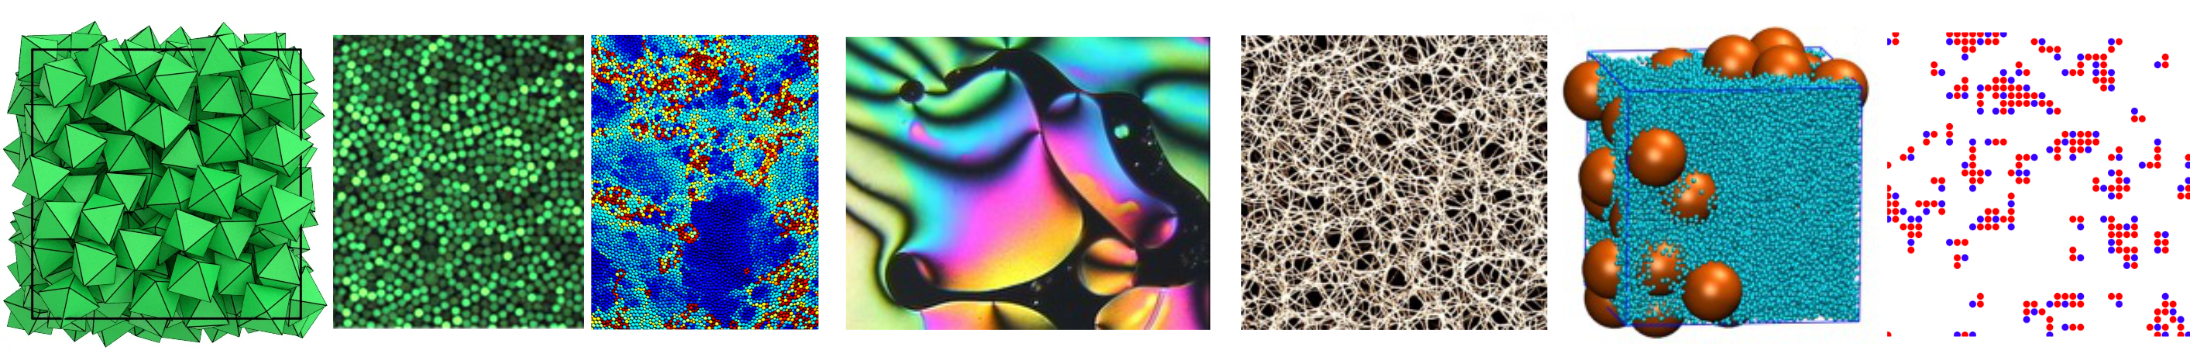
\includegraphics[keepaspectratio]{placeholder_figure_long.png}}\hfill

\section*{Overview}\label{overview}
\addcontentsline{toc}{section}{Overview}

\markright{Overview}

This course introduces your to the theoretical, computational and
experimental aspects of the physics of complex disordered matter.

Complex disordered matter is the study of wide range of systems like
\textbf{polymers}, \textbf{colloids}, \textbf{glasses}, \textbf{gels},
and \textbf{emulsions}, which lack long-range order but exhibit
intricate behaviour. Colloids, suspensions of microscopic particles in a
fluid, are useful for studying disordered structures due to their
observable dynamics. Similarly, polymer systems can form amorphous
solids or glasses when densely packed or cooled, showing solid-like
rigidity despite their disordered structure. These materials often
undergo phase transitions, such as demixing and crystallisation, and
near these transitions, they can display critical phenomena with
extensive fluctuations and correlations.

These various are examples of \textbf{soft matter}. systems In soft
matter systems, the interplay between disorder, softness, and phase
behavior leads to rich physical phenomena, particularly near critical
points where even small changes in external conditions can trigger
large-scale reorganizations and universal behaviour. Glasses, for
instance, exhibit slow relaxation and memory effects, while colloidal
systems may crystallize, phase separate, or become jammed depending on
particle interactions and concentration. Understanding such behaviors
involves studying how microscopic interactions and thermal fluctuations
influence macroscopic properties, especially in non-equilibrium
conditions. Through techniques like scattering, microscopy, rheology,
and simulation, one can explore how disordered soft materials respond to
stress, age, or undergo transitions---insights that are vital for
applications in materials design, biotechnology, and beyond.

This course is organized into three interconnected parts, each offering
a distinct perspective on the study of complex disordered matter.

\begin{itemize}
\tightlist
\item
  \textbf{Part 1: Unifying concepts} (Nigel Wilding) introduces the
  theoretical framework for rationalising complex disordered matter
  which is grounded in statistical mechanics and thermodynamics. We
  emphasize the theory of phase transitions, thermal fluctuations,
  critical phenomena, and stochastic dynamics---providing the essential
  theoretical tools needed to describe and predict the behavior of soft
  and disordered systems.\\
\item
  \textbf{Part 2: Complex disordered matter} (Francesco Turci) explores
  the phenomenology of key examples of complex disordered soft matter
  systems, including colloids, polymers, liquid crystals, glasses, gels,
  and active matter. These systems will be analyzed using the
  theoretical concepts introduced in Part 1, highlighting how disorder,
  interactions, and fluctuations shape their macroscopic behavior.\\
\item
  \textbf{Part 3: Experimental techniques} (Adrian Barnes) focuses on
  the methods of microscopy, and scattering via x-rays, neutrons and
  light that are used to study complex disordered matter, offering
  insight into how their properties are measured and understood in
  real-world contexts.
\end{itemize}

In addition to theory and experiment, computer simulation plays a
central role in soft matter research. This course includes a substantial
coursework component consisting of two computational projects. These
exercises will allow you to apply state-of-the-art simulation techniques
to investigate the complex behavior of disordered systems, bridging
theory and observation through hands-on exploration.

\section*{Delivery and format}\label{delivery-and-format}
\addcontentsline{toc}{section}{Delivery and format}

\markright{Delivery and format}

\begin{itemize}
\item
  Detailed e-notes (accessible via Blackboard) can be viewed on a
  variety of devices. Pdf is also available.
\item
  We will give `traditional' lectures (Tuesdays, Wednesdays, Fridays) in
  which we use slides to summarise and explain the lecture content.
  Questions are welcome (within reason\ldots)
\item
  Try to read ahead in the notes, then come to lectures, listen to the
  explanations and then reread the notes.
\item
  Rewriting the notes or slides to express your own thoughts and
  understanding, or annotating a pdf copy can help wire the material
  into your own way of thinking.
\item
  There are problem classes (Thursdays) where you can try problem sheets
  and seek help. Lecturers may go over some problems with the class.
\item
  The navigation bar on the left will allow you to access the lecture
  notes and problem sets.
\end{itemize}

\section*{Intended learning outcomes}\label{intended-learning-outcomes}
\addcontentsline{toc}{section}{Intended learning outcomes}

\markright{Intended learning outcomes}

The course will

\begin{itemize}
\tightlist
\item
  Introduce you to the qualitative features of a range of complex and
  disordered systems and the experimental techniques used to study them.
\item
  Introduce you to a range of model systems and theoretical techniques
  used to elucidate the physics of complex disordered matter.
\item
  Provide you with elementary computational tools to model complex
  disordered systems numerically and predict their properties.
\item
  Allow you to apply your physics background to understand a variety of
  systems of inter-disciplinary relevance.
\item
  Connect with the most recent advances in the research on complex
  disordered matter.
\end{itemize}

\section*{Contact details}\label{contact-details}
\addcontentsline{toc}{section}{Contact details}

\markright{Contact details}

The course will be taught by

\begin{itemize}
\tightlist
\item
  Prof Nigel B. Wilding (unit director): nigel.wilding@bristol.ac.uk
\item
  Dr Francesco Turci: F.Turci@bristol.ac.uk
\item
  Dr Adrian Barnes: a.c.barnes@bristol.ac.uk
\end{itemize}

\section*{Questions and comments}\label{questions-and-comments}
\addcontentsline{toc}{section}{Questions and comments}

\markright{Questions and comments}

If you have any questions about the course, please don't hesitate to
contact the relevant lecturer, either by email (see above) or in a
problems class.

Finally, this is a new course for 2025/26. If you find any errors or
mistakes or something which isn't clear, please let us know by email, or
fill in this anonymous form:

\begin{tcolorbox}[enhanced jigsaw, leftrule=.75mm, bottomrule=.15mm, colback=white, colframe=quarto-callout-note-color-frame, arc=.35mm, breakable, rightrule=.15mm, left=2mm, opacityback=0, toprule=.15mm]

\href{https://forms.office.com/e/6uL2Bd5QGq}{Submit an
error/mistake/query}

\end{tcolorbox}

\bookmarksetup{startatroot}

\chapter*{Recommended texts and literature}\label{literature}
\addcontentsline{toc}{chapter}{Recommended texts and literature}

\markboth{Recommended texts and literature}{Recommended texts and
literature}

\emph{Needs to be tidied and unified.}

\emph{Experimental textbooks?}

One motivation for supplying you with detailed notes for this course
course is the absence of a wholly ideal text book. However, it should be
stressed that while these notes approach (in places) the detail of a
book, the notes are not fully comprehensive and should be regarded as
the `bare bones' of the course, to be fleshed out via your own reading
and supplementary note taking. To this end perhaps the most appropriate
textbooks are:

A good book at the right level for the phase transitions and critical
phenomena part of the course is

\begin{itemize}
\tightlist
\item
  \textbf{\href{https://bris.on.worldcat.org/search/detail/24699159?queryString=yeomans\%20statistical&clusterResults=true&stickyFacetsChecked=true&groupVariantRecords=false&newsArticles=off&bookReviews=off}{J.M.
  Yeomans: Statistical Mechanics of Phase Transitions}}
\end{itemize}

A good book covering all aspects of this part of the course including
non-equilibrium systems is

\begin{itemize}
\tightlist
\item
  \textbf{\href{https://bris.on.worldcat.org/search/detail/941821555?queryString=chandler\%20statistical&clusterResults=true&stickyFacetsChecked=true&groupVariantRecords=false&newsArticles=off&bookReviews=off}{D.
  Chandler: Introduction to Modern Statistical Mechanics}}
\end{itemize}

You might also wish to dip into the introductory chapters of the
following more advanced texts

\begin{itemize}
\item
  \textbf{\href{https://bris.on.worldcat.org/search/detail/25914535?queryString=Lectures\%20on\%20Phase\%20Transitions\%20and\%20the\%20Renormalization\%20Group&clusterResults=true&stickyFacetsChecked=true&groupVariantRecords=false&newsArticles=off&bookReviews=off}{N
  Goldenfeld: Lectures on Phase Transitions and the Renormalization
  Group}}
\item
  \textbf{\href{https://bris.on.worldcat.org/search/detail/861559276?queryString=\%20The\%20Theory\%20of\%20Critical\%20Phenomena&clusterResults=true&stickyFacetsChecked=true&groupVariantRecords=false&newsArticles=off&bookReviews=off}{J.J.
  Binney, N.J. Dowrick, A.J.Fisher and M.E.J. Newman: The Theory of
  Critical Phenomena}}
\end{itemize}

For revision on thermodynamics and statistical mechanics

\begin{itemize}
\tightlist
\item
  \textbf{\href{https://bris.on.worldcat.org/search/detail/15487191?queryString=F.\%20Mandl&clusterResults=true&stickyFacetsChecked=true&groupVariantRecords=false}{F.
  Mandl: Statistical Physics}}.
\end{itemize}

For Stochastic dynamics

\begin{itemize}
\tightlist
\item
  \textbf{\href{https://bris.on.worldcat.org/search/detail/162131511?queryString=Stochastic\%20Processes\%20in\%20Physics\%20and\%20Chemistry\%20by\%20N.G.\%20van\%20Kampen&clusterResults=true&stickyFacetsChecked=true&groupVariantRecords=false}{N.G.
  van Kampen: Stochastic processess in Physics and Chemistry}}
\end{itemize}

The best overall text for part 2 of the course is: R.A.L Jones, Soft
Condensed Matter, Oxford University Press.

Additionally, the following more specialised texts should also be
useful. They can be found in the University Library under the stated
shelfmark.

\subsection*{Colloids}\label{colloids}
\addcontentsline{toc}{subsection}{Colloids}

\begin{enumerate}
\def\labelenumi{(\arabic{enumi})}
\tightlist
\item
  D.F.Evans, H.Wennerström: The Colloidal Domain - Where Physics,
  Chemistry, Biology, and Technology Meet. VCH Publishers (1994).
\item
  R.J.Hunter: Introduction to Modern Colloid Science. Oxford University
  Press (1993).
\item
  W.B.Russel, D.A.Saville, W.R.Schowalter: Colloidal Dispersions
  Cambridge University Press (1989).
\item
  D.H.Everett: Basic Principles of Colloid Science.
\end{enumerate}

Royal Society of Chemistry Paperbacks (1988)

\subsection*{Polymers and surfactants}\label{polymers-and-surfactants}
\addcontentsline{toc}{subsection}{Polymers and surfactants}

\begin{enumerate}
\def\labelenumi{(\arabic{enumi})}
\tightlist
\item
  R.J. Young and P.A. Lovell: Introduction to polymers .
\item
  M. Doi: Introduction to polymer physics
\item
  J.Israelachvili, Intermolecular and Surface Forces, Academic Press
  (1992), Chs. 16 and 17
\end{enumerate}

\subsection*{Glasses}\label{glasses}
\addcontentsline{toc}{subsection}{Glasses}

\begin{enumerate}
\def\labelenumi{(\arabic{enumi})}
\tightlist
\item
  J. Zarzycki; Glasses and the vitreous state. Cambridge University
  Press (1991).
\end{enumerate}

\part{Unifying concepts}

\chapter{Introduction to phase behaviour and enhanced
fluctuations}\label{introduction-to-phase-behaviour-and-enhanced-fluctuations}

A phase transition can be defined as a macroscopic rearrangment of the
internal constituents of a system in response to a change in the
thermodynamic conditions to which they are subject. A wide variety of
physical systems undergo such transitions. Understanding the properties
of phase transitions is fundamental to the study of soft and complex
matter, as these systems often exhibit rich and subtle transformations
between different states of organization. Whether in colloidal
suspensions, polymer blends, liquid crystals, or biological materials,
phase transitions underpin a wide range of physical behaviours, from
self-assembly and pattern formation to critical phenomena and dynamical
arrest. By analysing how macroscopic phases emerge from microscopic
interactions and external conditions, one gains crucial insight into the
principles that govern structure, stability, and functionality in these
intricate systems. As such, an understanding of phase transitions not
only enriches theoretical understanding but also informs practical
applications across materials science, biophysics, and nanotechnology.
For these reasons we will devote a large proportion of this course to
the study of phase transitions.

Two classic examples of systems displaying phase transitions are the
ferromagnet and fluid systems. For the magnet, a key observable is the
magnetisation defined as the magnetic moment per spin, given by
\(m=M/N\), with \(N\) the number of spins. \(m\) can be positive or
negative, dependent on whether the spins are aligned `up' or `down'. As
the temperature of a ferromagnet is increased, its net magnetisation
\(|m|\) is observed to decrease smoothly, until at a certain temperature
known as the critical temperature, \(T_c\), it vanishes altogether (see
left part of Figure~\ref{fig-isingpd}). We define the magnetisation to
be the \emph{order parameter} of this phase transition.

One can also envisage applying a magnetic field \(H\) to the system
which, depending on its sign (i.e.~whether it is aligned (positive) or
anti-aligned (negative) relative to the magnetisation axis), favours up
or down spin states respectively, as shown schematically in
Figure~\ref{fig-isingpd} (right part). Changing the sign of the magnetic
field \(H\) for \(T<T_c\) leads to a phase transition chacterised by a
discontinuous jump in \(m\). We shall explore this behaviour in more
detail in section 6.

\begin{figure}

\centering{

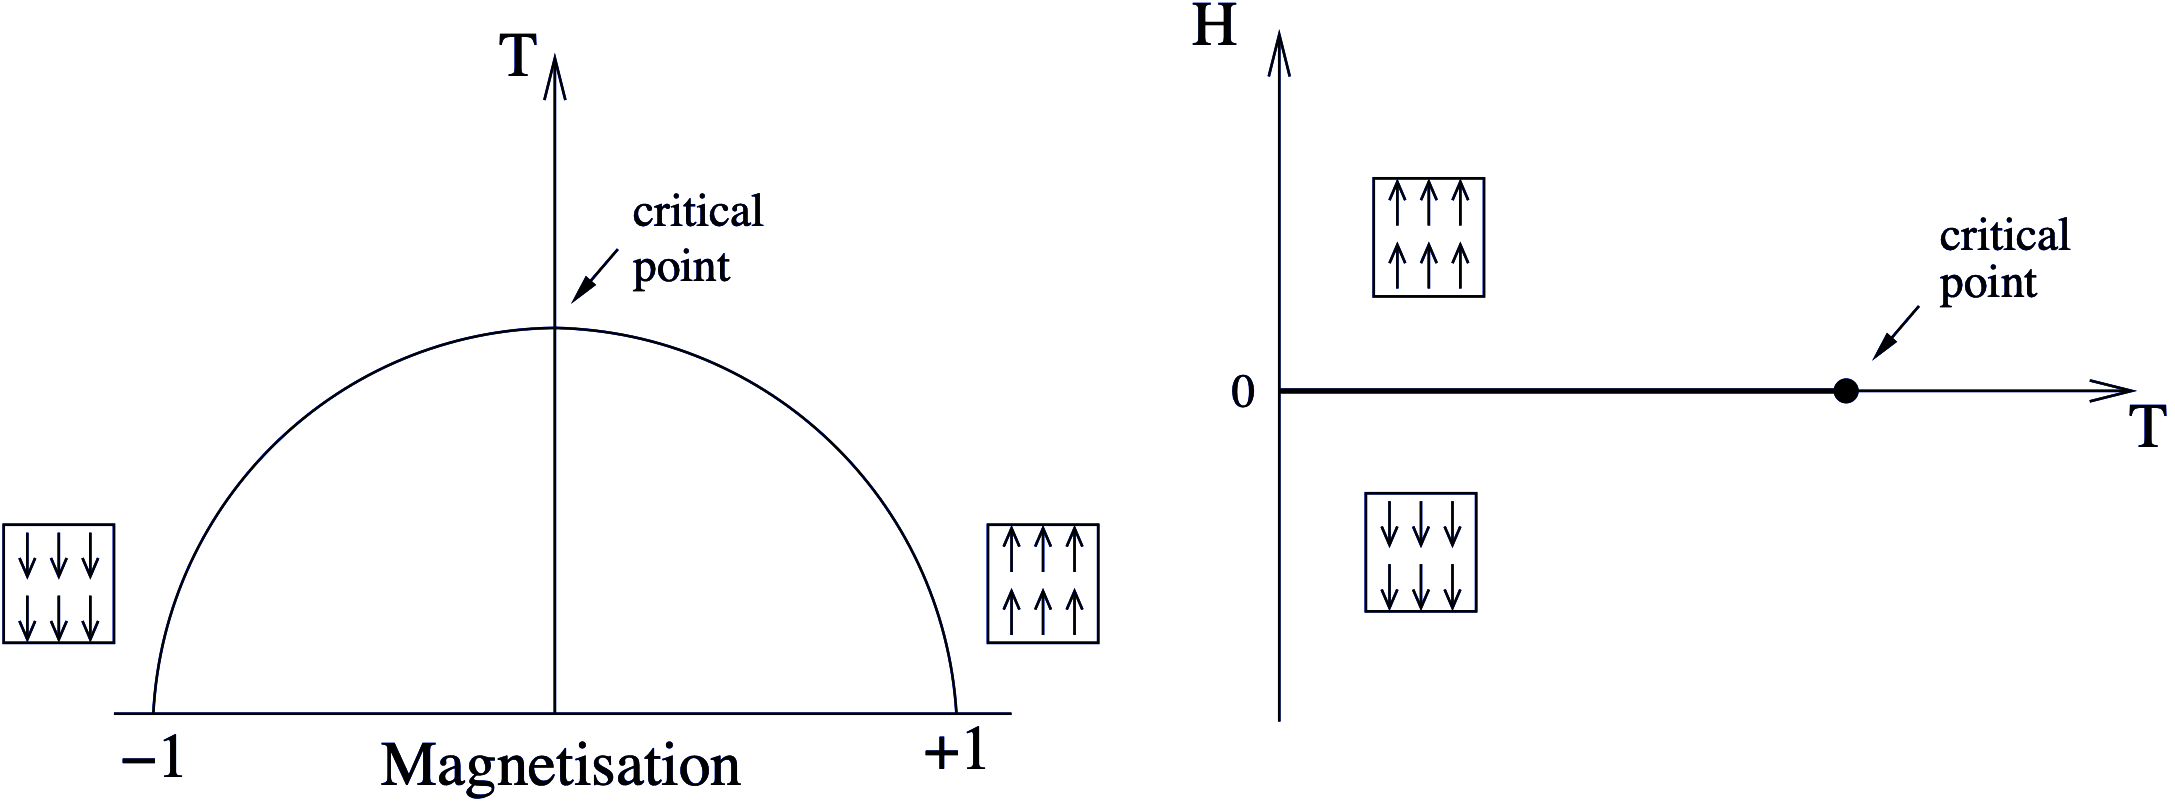
\includegraphics[width=0.8\linewidth,height=\textheight,keepaspectratio]{phase-transitions/Figs/isingpd_color.png}

}

\caption{\label{fig-isingpd}Phase diagram of a simple magnet
(schematic). Left: magnetisation as a function of temperature for zero
applied magnetic field, \(H=0\). Right: Applying a magnetic field that
is aligned or antialigned with the direction of the magnetisation leads
to a phase transition. The \(H=0\) axis at \(T<T_c\) is the coexistence
curve for which positive and negative magnetisations are equally
likely.}

\end{figure}%

Similarly, a change of state from liquid to gas can be induced in a
fluid system (though not in an ideal gas) simply by raising the
temperature. Typically the liquid-vapour transition is abrupt,
reflecting the large number density difference between the states either
side of the transition. However the abruptness of this transition can be
reduced by applying pressure. At one particular pressure and temperature
the discontinuity in the density difference between the two states
vanishes and the two phases coalesce. These conditions of pressure and
temperature serve to locate the critical point for the fluid. We define
the density difference \(\rho_{liq}-\rho_{vap}\) to be the order
parameter for the liquid-gas phase transition. We shall meet order
parameters for other, more complex, systems in
Section~\ref{sec-landau-theory},

\begin{figure}

\centering{

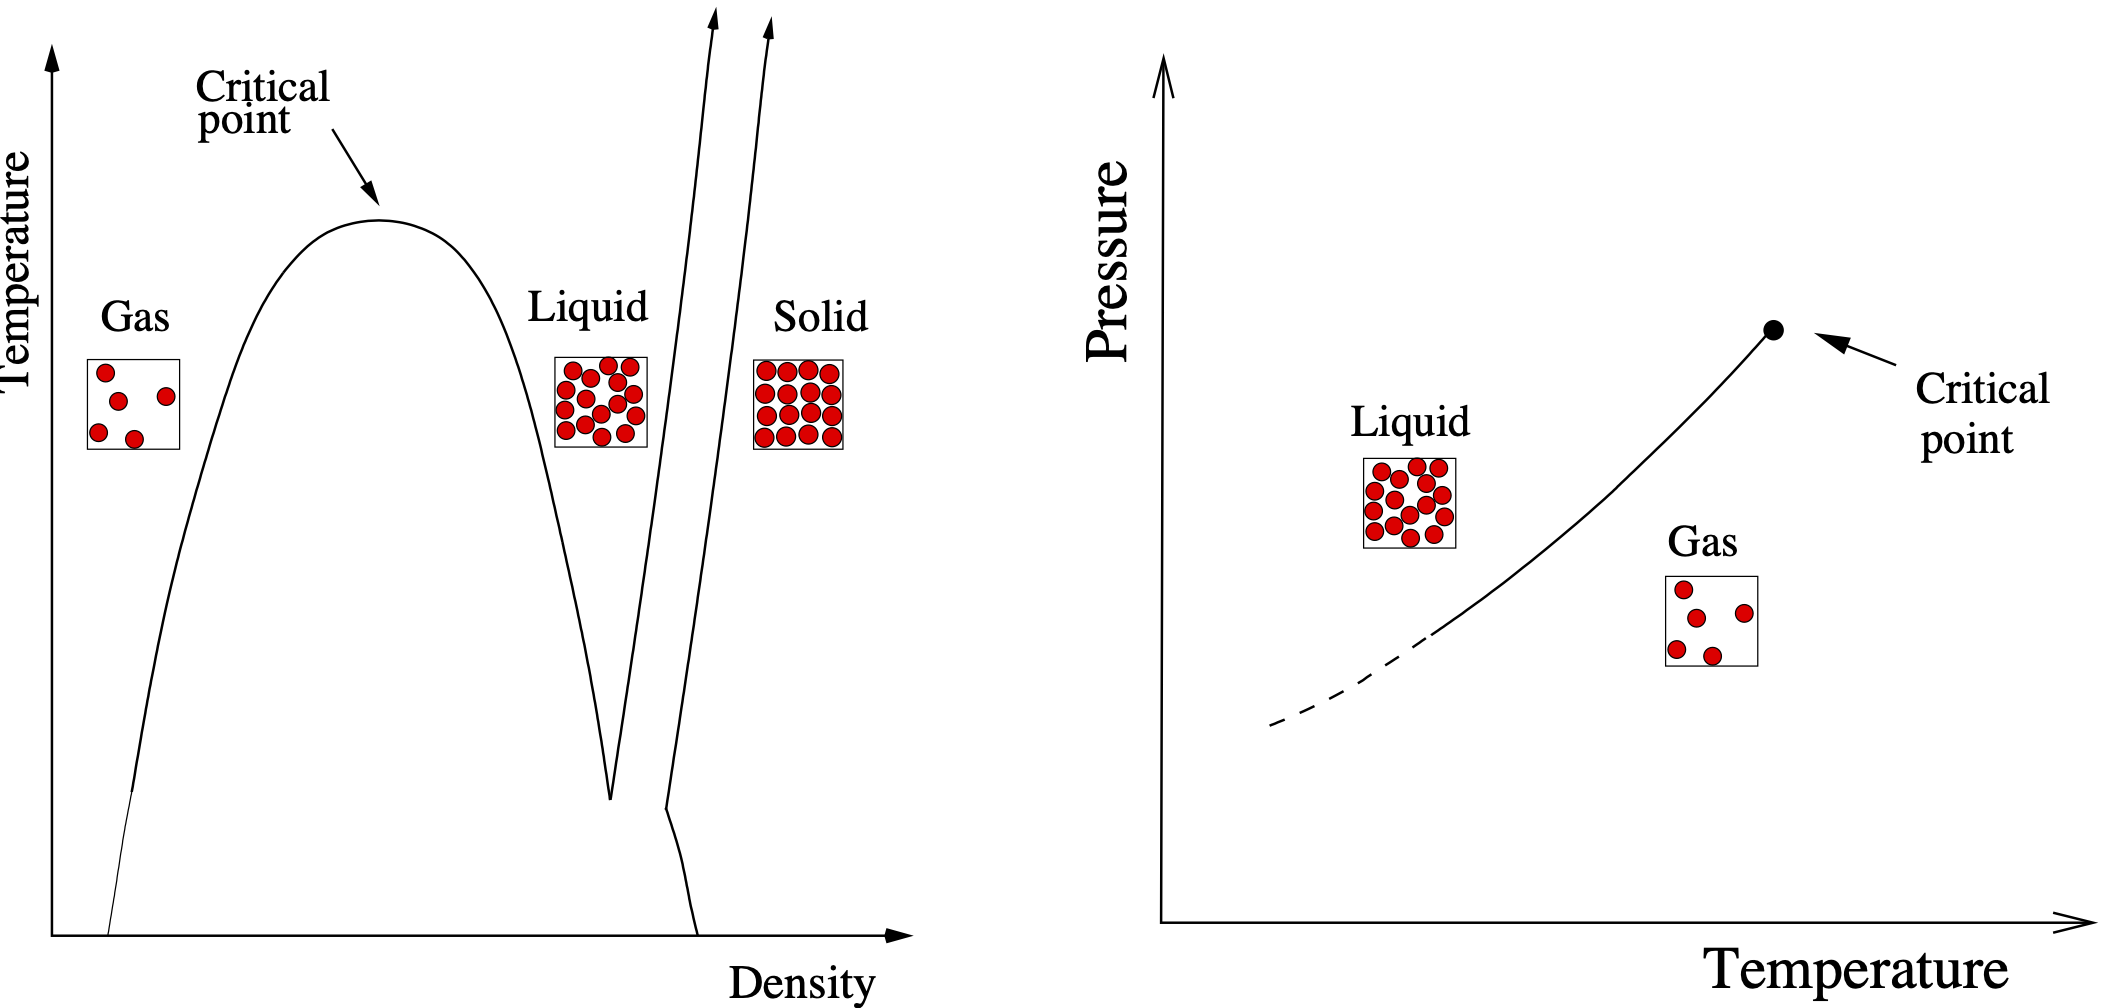
\includegraphics[width=0.8\linewidth,height=\textheight,keepaspectratio]{phase-transitions/Figs/ljpd1.png}

}

\caption{\label{fig-fluidpd}Phase diagram of a simple fluid (schematic)}

\end{figure}%

In the vicinity of a critical point, a system displays a host of
remarkable behaviors known as \emph{critical phenomena}. Chief among
these is the divergence of thermal response functions---such as specific
heat, compressibility, or magnetic susceptibility---which signal an
enhanced sensitivity to external perturbations. These singularities
arise from the emergence of large-scale cooperative interactions among
the system's microscopic constituents, as measured by a diverging
\emph{correlation length} (see Chapter~\ref{sec-background}). One
visually striking manifestation of this is \emph{critical opalescence},
particularly observed in fluids like CO\(_2\). As carbon dioxide nears
its critical temperature and pressure, the distinction between its
liquid and gas phases vanishes, giving rise to huge fluctuations in
density. These fluctuations scatter visible light, rendering the fluid
milky or opalescent. This scattering effect directly reflects the
long-range correlations developing within the fluid. The movie below
illustrates the effect as the critical temperature of CO\(_2\) is
approached from above. Note the appearence of a liquid-vapour interface
(meniscus) as the system enters the two-phase region.

\url{Movies/critical_point_1.mp4}

The recalcitrant problem posed by the critical region is how best to
incorporate such collective effects within the framework of a rigorous
mathematical theory that affords both physical insight and quantitative
explanation of the observed phenomena. This matter has been (and still
is!) the subject of intense theoretical activity.

The importance of the critical point stems largely from the fact that
many of the phenomena observed in its vicinity are believed to be common
to a whole range of apparently quite disparate physical systems. Systems
such as liquid mixtures, superconductors, liquid crystals, ferromagnets,
antiferromagnets and molecular crystals may display identical behaviour
near criticality. This observation implies a profound underlying
similarity among physical systems at criticality, regardless of many
aspects of their distinctive microscopic nature. These ideas have found
formal expression in the so-called `universality hypothesis' which,
since its inception in the 1970s, has enjoyed considerable success.

In the next few lectures, principal aspects of the contemporary
theoretical viewpoint of phase transitions and critical phenomena will
be reviewed. Mean field theories of phase transitions will be discussed
and their inadequacies in the critical region will be exposed. The
phenomenology of the critical region will we described including power
laws, critical exponents and their relationship to scaling phenomena.
These will be set within the context of the powerful renormalisation
group technique. The notion of universality as a phenomenological
hypothesis will be introduced and its implications for real and model
systems will be explored. Finally, the utility of finite-size scaling
methods for computer studies of critical phenomena will be discussed,
culminating in the introduction of a specific technique suitable for
exposing universality in model systems. Thereafter we will consider some
foundational concepts in the dynamics of complex disorderd matters. We
shall look at the processes by which one phase transform into another
and introduce differential equations that allow us to deal with the
inherent stochasticity of thermal systems. The wider applicability of
these unifying concepts to complex disordered systems such as colloids,
polymers, liquid crystals and glasses will be covered in part 2 of the
course.

\chapter{Key concepts for phase transitions}\label{sec-background}

\section{Observables and expectation
values}\label{observables-and-expectation-values}

In seeking to describe phase transition and critical phenomena, it is
useful to have a quantitative measure of the difference between the
phases: this is the role of the \emph{order parameter}, \(Q\). In the
case of the fluid, the order parameter is taken as the difference
between the densities of the liquid and vapour phases. In the
ferromagnet it is taken as the magnetisation. As its name suggest, the
order parameter serves as a measure of the kind of orderliness that sets
in when the temperature is cooled below a critical temperature.

Our first task is to give some feeling for the principles which underlie
the ordering process. Referring back to \textbf{?@sec-canonical}, the
probability \(p_a\) that a physical system at temperature \(T\) will
have a particular microscopic arrangement (alternatively referred to as
a `configuration' or `state'), labelled \(a\), of energy \(E_a\) is

\begin{equation}\phantomsection\label{eq-probs}{
p_a=\frac{1}{Z}e^{-E_a/k_BT}
}\end{equation}

The prefactor \(Z^{-1}\) is the \emph{partition function}: since the
system must always have \emph{some} specific arrangement, the sum of the
probabilities \(p_a\) must be unity, implying that

\begin{equation}\phantomsection\label{eq-partition}{
Z=\sum_ae^{-E_a/k_BT}
}\end{equation} where the sum extends over all possible microscopic
arrangements.

These equations assume that physical system evolves rapidly (on the
timescale of typical observations) amongst all its allowed arrangements,
sampling them with the probabilities~Equation~\ref{eq-probs} the
expectation value of any physical observable \(O\) will thus be given by
averaging \(O\) over all the arrangements \(a\), weighting each
contribution by the appropriate probability:

\begin{equation}\phantomsection\label{eq-observable}{\overline {O}=\frac{1}{Z}\sum_a O_a e^{-E_a/k_BT}
}\end{equation}

Sums like Equation~\ref{eq-observable} are not easily evaluated.
Nevertheless, some important insights follow painlessly. Consider the
case where the observable of interest is the order parameter, or more
specifically the magnetisation of a ferromagnet.

\begin{equation}\phantomsection\label{eq-op}{
Q=\frac{1}{Z}\sum_a Q_a e^{-E_a/k_BT}
}\end{equation}

It is clear from Equation~\ref{eq-probs} that at very low temperature
the system will be overwhelmingly likely to be found in its minimum
energy arrangements (ground states). For the ferromagnet, these are the
fully ordered spin arrangements having magnetisation \(+1\), or \(-1\).

Now consider the high temperature limit. The enhanced weight that the
fully ordered arrangement carries in the sum of Equation~\ref{eq-op} by
virtue of its low energy, is now no longer sufficient to offset the fact
that arrangements in which \(Q_a\) has some intermediate value, though
each carry a smaller weight, are vastly greater in number. A little
thought shows that the arrangements which have essentially zero
magnetisation (equal populations of up and down spins) are by far the
most numerous. At high temperature, these disordered arrangements
dominate the sum in Equation~\ref{eq-op} and the order parameter is
zero.

The competition between energy-of-arrangements weighting (or simply
`energy') and the `number of arrangements' weighting (or `entropy') is
then the key principle at work here. The distinctive feature of a system
with a critical point is that, in the course of this competition, the
system is forced to choose amongst a number of macroscopically different
sets of microscopic arrangements.

Finally in this section, we note that the probabilistic (statistical
mechanics) approach to thermal systems outlined above is completely
compatible with classical thermodynamics. Specifically, the bridge
between the two disciplines is provided by the following equation

\begin{equation}\phantomsection\label{eq-free}{
F=-k_BT \ln Z
}\end{equation}

where \(F\) is the ``Helmholtz free energy''. All thermodynamic
observables, for example the order parameter \(Q\), and response
functions such as the specific heat or magnetic susceptibility are
obtainable as appropriate derivatives of the free energy. For instance,
utilizing Equation~\ref{eq-partition}, one can readily verify (try it as
an exercise!) that the average internal energy is given by

\[\overline{E}=-\frac{\partial \ln Z}{\partial \beta},\]

where \(\beta=(k_BT)^{-1}\).

The relationship between other thermodynamic quantities and derivatives
of the free energy are given in fig. Figure~\ref{fig-thermo}

\begin{figure}

\centering{

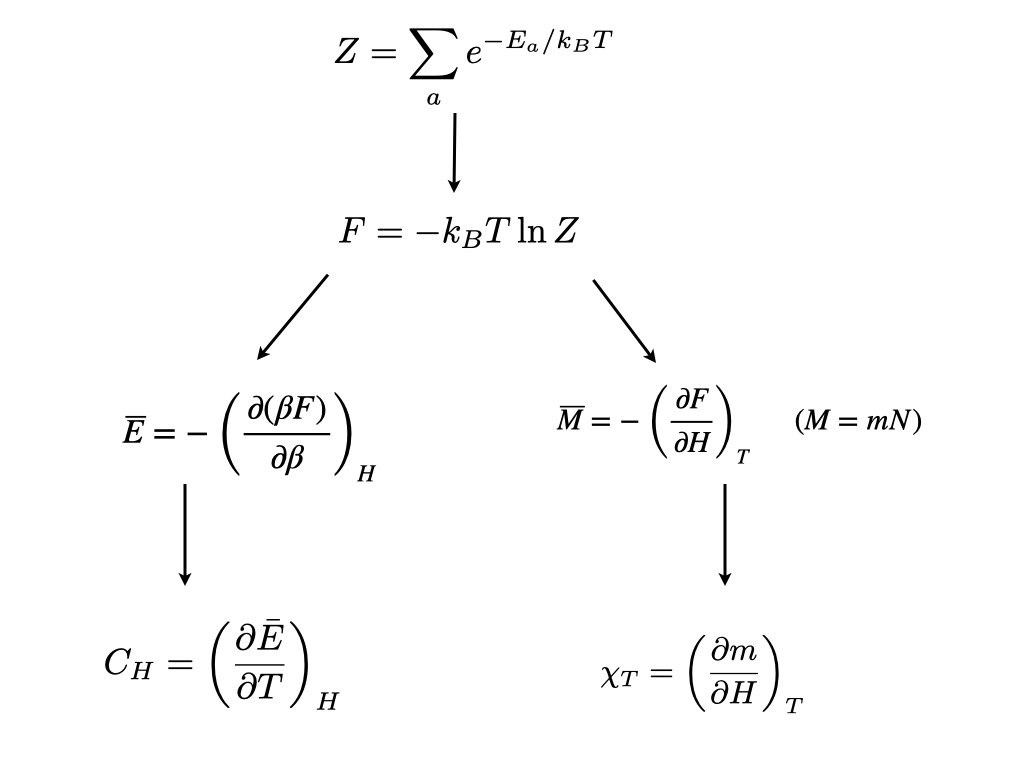
\includegraphics[width=0.8\linewidth,height=\textheight,keepaspectratio]{phase-transitions/Figs/thermo.png}

}

\caption{\label{fig-thermo}Relationships between the partition function
and thermodynamic observables}

\end{figure}%

\section{Correlations}\label{sec-correlations}

\subsection{Spatial correlations}\label{spatial-correlations}

The two-point connected correlation function measures how fluctuations
at two spatial points are statistically related. For a scalar field
\(\phi(\vec{R})\), which could represent eg. the local magnetisation
\(m\) in a magnet at position vector \(\vec{R}\), or the local particle
number density \(\rho\) in a fluid, it is defined as:

\[
C(r) = \langle \phi(\vec{R}) \phi(\vec{R} + \vec{r}) \rangle - \langle \phi(\vec{R}) \rangle^2,
\]

where \(\langle \cdot \rangle\) denotes an ensemble or spatial average
over all \(\vec{R}\), and \(r = |\vec{r}|\) is the spatial separation
between the two points.

\(C(r)\) quantifies the spatial extent over which field values are
correlated and in homogeneous and isotropic systems, it depends only on
the separation \(r\).

If \(C(r)\) decays quickly, we say that correlations are short-ranged.
Typically this occurs well away from criticality and takes the form of
exponential decay

\[
  C(r) \sim e^{-r/\xi}
  \] where the correlation length \(\xi\) is the characteristic scale
over which correlations decay.

Near a critical point \(C(r)\) decays more slowly - in a power-law
fashion - and correlations are long-ranged.

\[
  C(r) \sim r^{-(d - 2 + \eta)}
  \] where \(d\) is the spatial dimension and \(\eta\) is a critical
exponent.

In isotropic fluids and particle systems, a closely related and more
directly measurable quantity (particularly in simulations) is the
\textbf{radial distribution function} \(g(r)\), which describes how
particle density varies as a function of distance from a reference
particle. For such systems, the two-point correlation function of the
number density field \(\rho(\vec{r})\) is related to \(g(r)\) as
follows:

\[
g(r) = 1+\frac{C(r)}{\rho^2},
\] where \(\rho\) is the average number density. This relation shows
that \(g(r)\) encodes the same spatial correlations as \(C(r)\), but in
a form that is more natural for discrete particle systems. Note that by
definition \(g(r)\to 1\) in the absence of correlations ie. when
\(C(r)=0\). This is typically the case for \(r\gg\xi\).

Experimentally one doesn't typically have direct access to \(C(r)\), but
rather its Fourier transform known as the \textbf{structure factor}

\[
S(k) = \int d^d r \, e^{-i \vec{k} \cdot \vec{r}} \, C(r),
\] where \(k\) is the scattering wavevector.

In equilibrium:

\begin{itemize}
\item
  For short-range correlations (finite \(\xi\)), \(S(k)\) typically has
  a Lorentzian form: \[
  S(k) \sim \frac{1}{k^2 + \xi^{-2}}.
  \]
\item
  At criticality (where \(\xi \to \infty\)), \(S(k)\) follows a power
  law: \[
  S(k) \sim k^{-2 + \eta}.
  \]
\end{itemize}

This relation enables the extraction of \(\xi\) from experimental or
simulation data, especially via scattering techniques.

\subsection{Temporal correlations}\label{temporal-correlations}

Consider a thermodynamic variable \(x\) with zero mean that fluctuates
over time. Examples include the local magnetization in a magnetic system
or the local density in a fluid. Here, \(x\) represents a deviation from
the average value --- a fluctuation.

We're interested in how such fluctuations are correlated over time when
the system is in thermal equilibrium. For instance, if \(x\) is positive
at some time \(t\), it's more likely to remain positive shortly after.

These temporal correlations are characterized by the two-time
correlation function (also known as an auto-correlation function):

\[
\langle x(\tau) x(\tau + t) \rangle
\]

In equilibrium, the correlation function must be independent of the
starting time \(\tau\). Therefore, we define:

\[
\langle x(\tau) x(\tau + t) \rangle = M_{xx}(t)
\]

That is, \(M_{xx}(t)\) depends only on the time difference \(t\).

We typically expect \(M_{xx}(t)\) to decay exponentially over a
characteristic correlation time \(t_c\):

\[
M_{xx}(t) \sim \exp(-t / t_c)
\]

\begin{figure}

\centering{

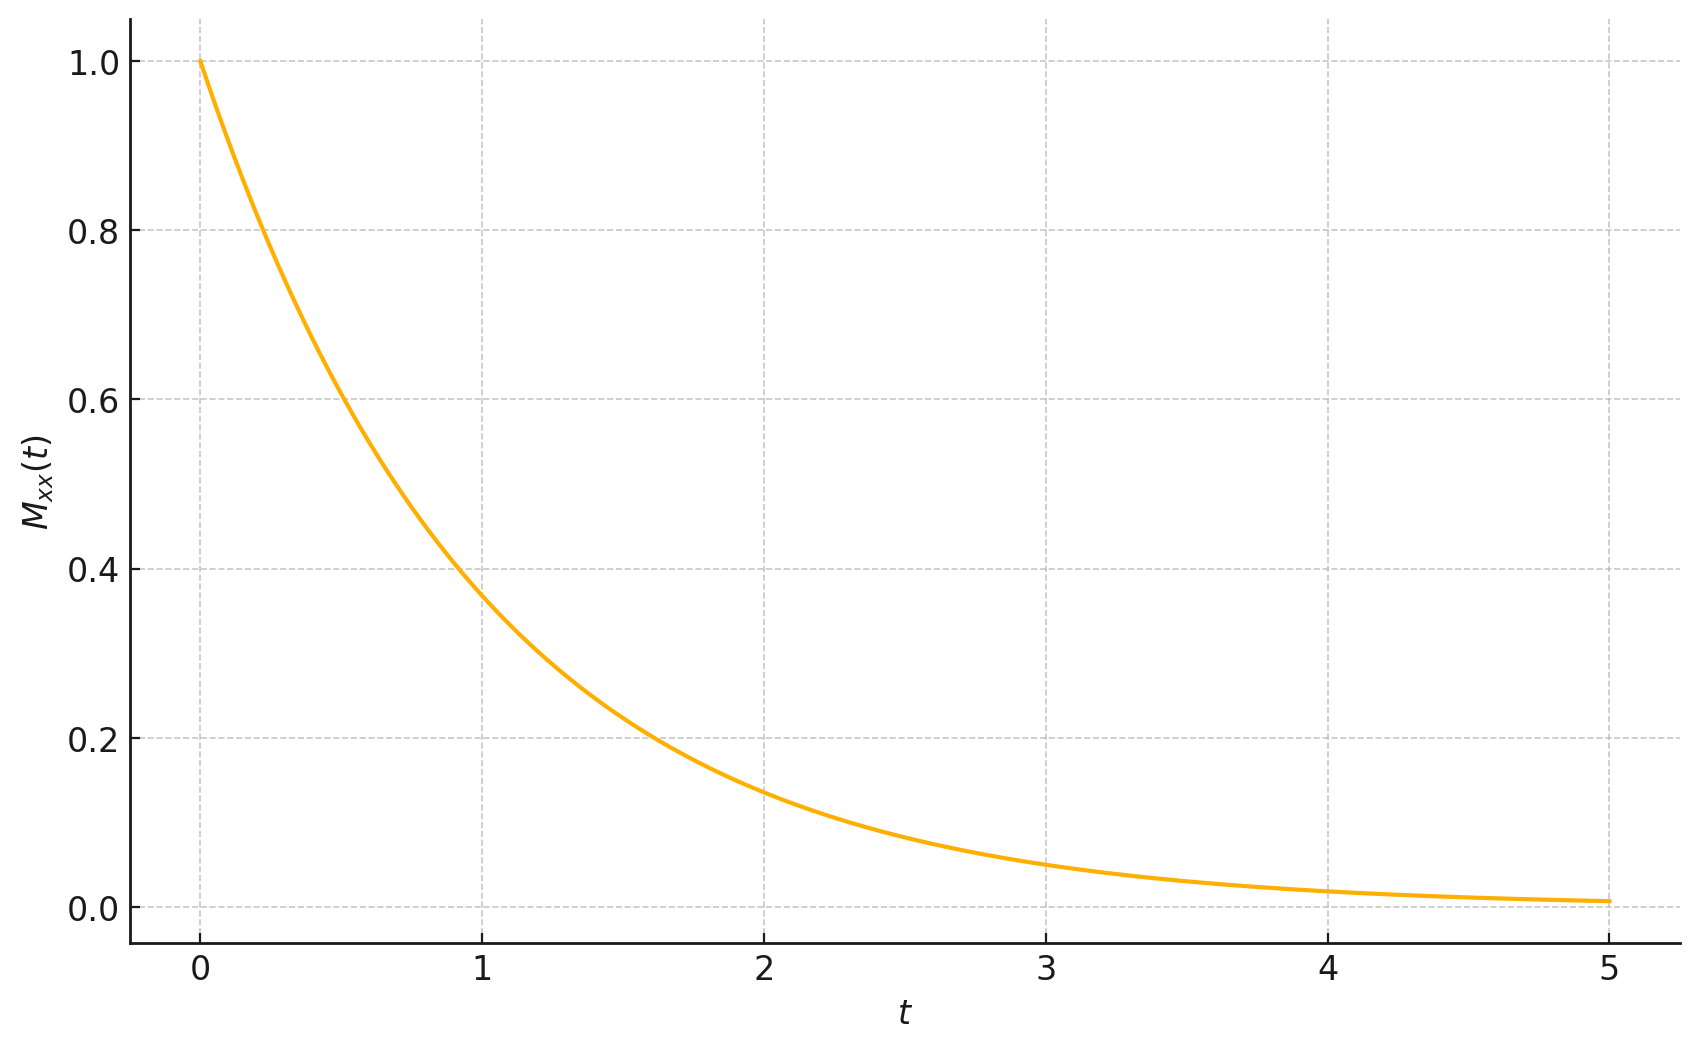
\includegraphics[width=0.6\linewidth,height=\textheight,keepaspectratio]{phase-transitions/Figs/Mxx(t).png}

}

\caption{\label{fig-Mxx}Sketch of \(M_{xx}(t)\) against \(t\)}

\end{figure}%

This exponential decay reflects how the memory of fluctuations fades
with time.

Now consider two different fluctuating variables, \(x\) and \(y\) (e.g.,
local magnetizations at different positions). Their cross-correlation
function is defined as:

\[
\langle x(\tau) y(\tau + t) \rangle = M_{xy}(t)
\]

This defines the elements of a dynamic correlation matrix, of which
\(M_{xx}(t)\) is the diagonal.

\chapter{The Approach to Criticality}\label{sec:approach}

It is a matter of experimental fact that the approach to criticality in
a given system is characterized by the divergence of various
thermodynamic observables. Let us remain with the archetypal example of
a critical system, the ferromagnet, whose critical temperature will be
denoted as \(T_c\). For temperatures close to \(T_c\), the magnetic
response functions (the magnetic susceptibility \(\chi\) and the
specific heat) are found to be singular functions, diverging as a
\emph{power} of the reduced (dimensionless) temperature \(t \equiv
(T-T_c)/T_c\):-

\begin{equation}\phantomsection\label{eq-chipow}{
\chi \equiv \frac{\partial M}{\partial H}\propto t^{-\gamma} ~~~~ (H=0) 
}\end{equation}

(where \(M=mN\)), \begin{equation}\phantomsection\label{eq-Cv}{
C_H \equiv \frac{\partial E}{\partial T}\propto t^{-\alpha} ~~~~ (H=\textrm{ constant}) 
}\end{equation}

Another key quantity is the correlation length \(\xi\), which measures
the distance over which fluctuations of the magnetic moments are
correlated. This is observed to diverge near the critical point with an
exponent \(\nu\).

\begin{equation}\phantomsection\label{eq-corr}{
\xi \propto t^{-\nu} ~~~~ (T > T_c,\: H=0)
}\end{equation}

Similar power law behaviour is found for the order parameter \(Q\) (in
this case the magnetisation) which vanishes in a singular fashion (it
has infinite gradient) as the critical point is is approached as a
function of temperature:

\begin{equation}\phantomsection\label{eq-mag}{
m \propto t^{\beta} ~~~~ (T < T_c,\: H=0) 
}\end{equation} (here the symbol \(\beta\), is not to be confused with
\(\beta=1/k_BT\)-- this unfortunately is the standard notation.)

Finally, as a function of magnetic field:

\begin{equation}\phantomsection\label{eq-field}{m \propto h^{1/\delta} ~~~~ (T = T_c,\: H>0) .}\end{equation}
with \(h=(H-H_c)/H_c\), the reduced magnetic field.

As examples, the behaviour of the magnetisation and correlation length
are plotted in Figure~\ref{fig-sing} as a function of \(t\).

\begin{figure}

\centering{

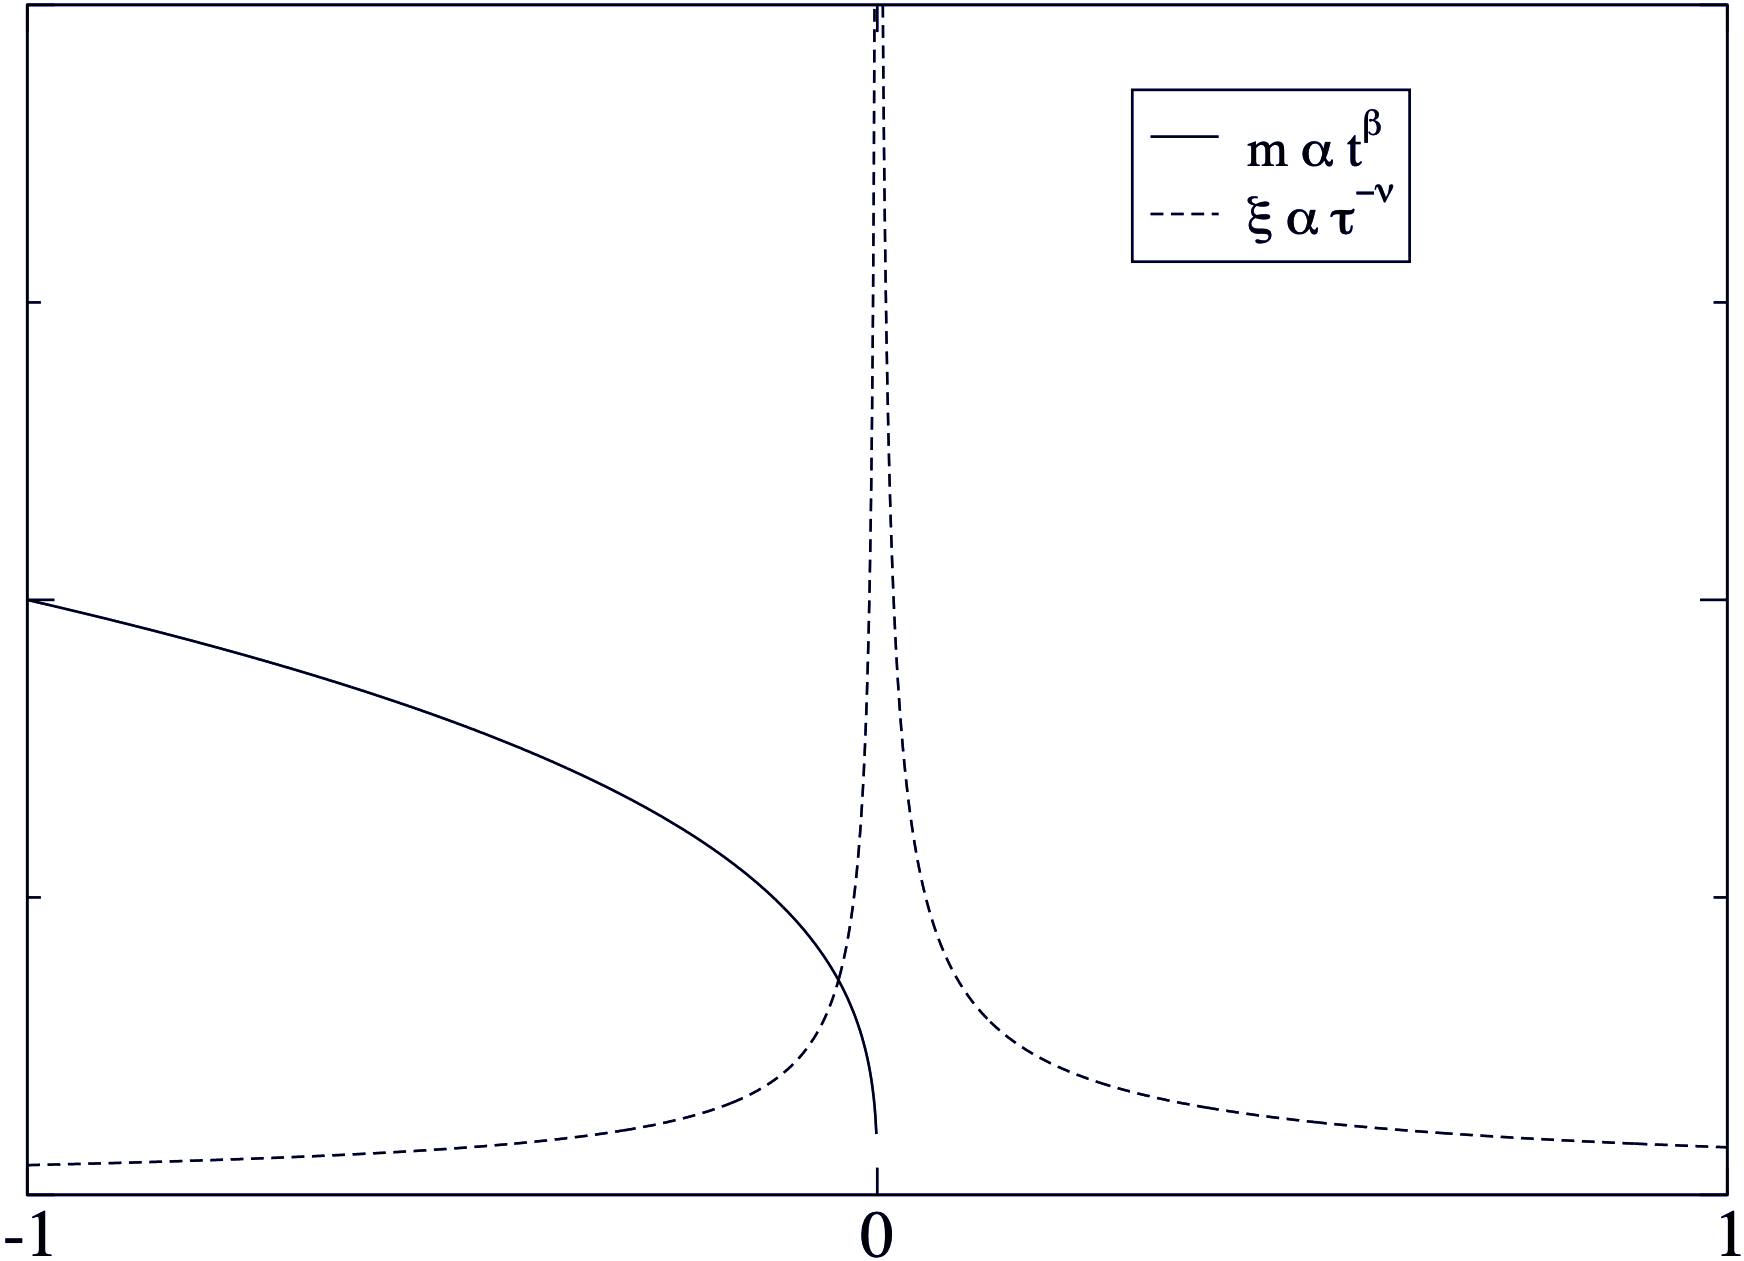
\includegraphics[width=0.5\linewidth,height=\textheight,keepaspectratio]{phase-transitions/Figs/sing_color.png}

}

\caption{\label{fig-sing}Singular behaviour of the correlation length
and order parameter in the vicinity of the critical point as a function
of the reduced temperature \(t\).}

\end{figure}%

The quantities \(\gamma, \alpha, \nu, \beta\) in the above equations are
known as critical exponents. They serve to control the rate at which the
various thermodynamic quantities change on the approach to criticality.

Remarkably, the form of singular behaviour observed at criticality for
the example ferromagnet also occurs in qualitatively quite different
systems such as the fluid. All that is required to obtain the
corresponding power law relationships for the fluid is to substitute the
analogous thermodynamic quantities in to the above equations.
Accordingly the magnetisation order parameter is replaced by the density
difference \(\rho_{liq}-\rho_{gas}\) while the susceptibility is
replaced by the isothermal compressibility and the specific heat
capacity at constant field is replaced by the specific heat capacity at
constant volume. The approach to criticality in a variety of
qualitatively quite different systems can therefore be expressed in
terms of a set of critical exponents describing the power law behaviour
for that system (see the book by Yeomans for examples).

Even more remarkable is the experimental observation that the values of
the critical exponents for a whole range of fluids and magnets (and
indeed many other systems with critical points) are \emph{identical}.
This is the phenomenon of \emph{universality}. It implies a deep
underlying physical similarity between ostensibly disparate critical
systems. The principal aim of theories of critical point phenomena is to
provide a sound theoretical basis for the existence of power law
behaviour, the factors governing the observed values of critical
exponents and the universality phenomenon. Ultimately this basis is
provided by the Renormalisation Group (RG) theory, for which K.G. Wilson
was awarded the Nobel Prize in Physics in 1982.

More about the scientists mentioned in this chapter:

\href{https://en.wikipedia.org/wiki/Kenneth_G._Wilson}{Kenneth Wilson}

\chapter{The Ising model: the prototype model for a phase
transition}\label{sec:models}

In order to probe the properties of the critical region, it is common to
appeal to simplified model systems whose behaviour parallels that of
real materials. The sophistication of any particular model depends on
the properties of the system it is supposed to represent. The simplest
model to exhibit critical phenomena is the two-dimensional Ising model
of a ferromagnet. Actual physical realizations of 2-d magnetic systems
do exist in the form of layered ferromagnets such as K\(_2\)CoF\(_4\),
so the 2-d Ising model is of more than just technical relevance.

\section{The 2D Ising model}\label{the-2d-ising-model}

The 2-d spin-\(\frac{1}{2}\) Ising model envisages a regular arrangement
of magnetic moments or `spins' on an infinite plane. Each spin can take
two values, \(+1\) (`up' spins) or \(-1\) (`down' spins) and is assumed
to interact with its nearest neighbours according to the Hamiltonian

\begin{equation}\phantomsection\label{eq-ising}{
{\cal H}_I=-J\sum_{<ij>}s_is_j - H\sum_i s_i
}\end{equation}

where \(J>0\) measures the strength of the coupling between spins and
the sum extends over nearest neighbour spins \(s_i\) and \(s_j\), i.e it
is a sum of the bonds of the lattice. \(H\) is a magnetic field term
which can be positive or negative (although for the time being we will
set it equal to zero). The order parameter is simply the average
magnetisation:

\[m=\frac{1}{N} \langle \sum_i s_i \rangle\:,\] where
\(\langle\cdot\rangle\) means an average over configurations.

The fact that the Ising model displays a phase transition was argued in
Chapter~\ref{sec-background}. Thus at low temperatures for which there
is little thermal disorder, there is a preponderance of aligned spins
and hence a net spontaneous magnetic moment (ie. the system is
ferromagnetic). As the temperature is raised, thermal disorder increases
until at a certain temperature \(T_c\), entropy drives the system
through a continuous phase transition to a disordered spin arrangement
with zero net magnetisation (ie. the system is paramagnetic). These
trends are visible in configurational snapshots from computer
simulations of the 2D Ising model (see Figure~\ref{fig-snapshots}).
Although each spin interacts only with its nearest neighbours, the phase
transition occurs due to cooperative effects among a large number of
spins. In the neighbourhood of the transition temperature these
cooperative effects engender fluctuations that can extend over all
length-scales from the lattice spacing up to the correlation length.

\begin{figure}

\begin{minipage}{0.33\linewidth}

\pandocbounded{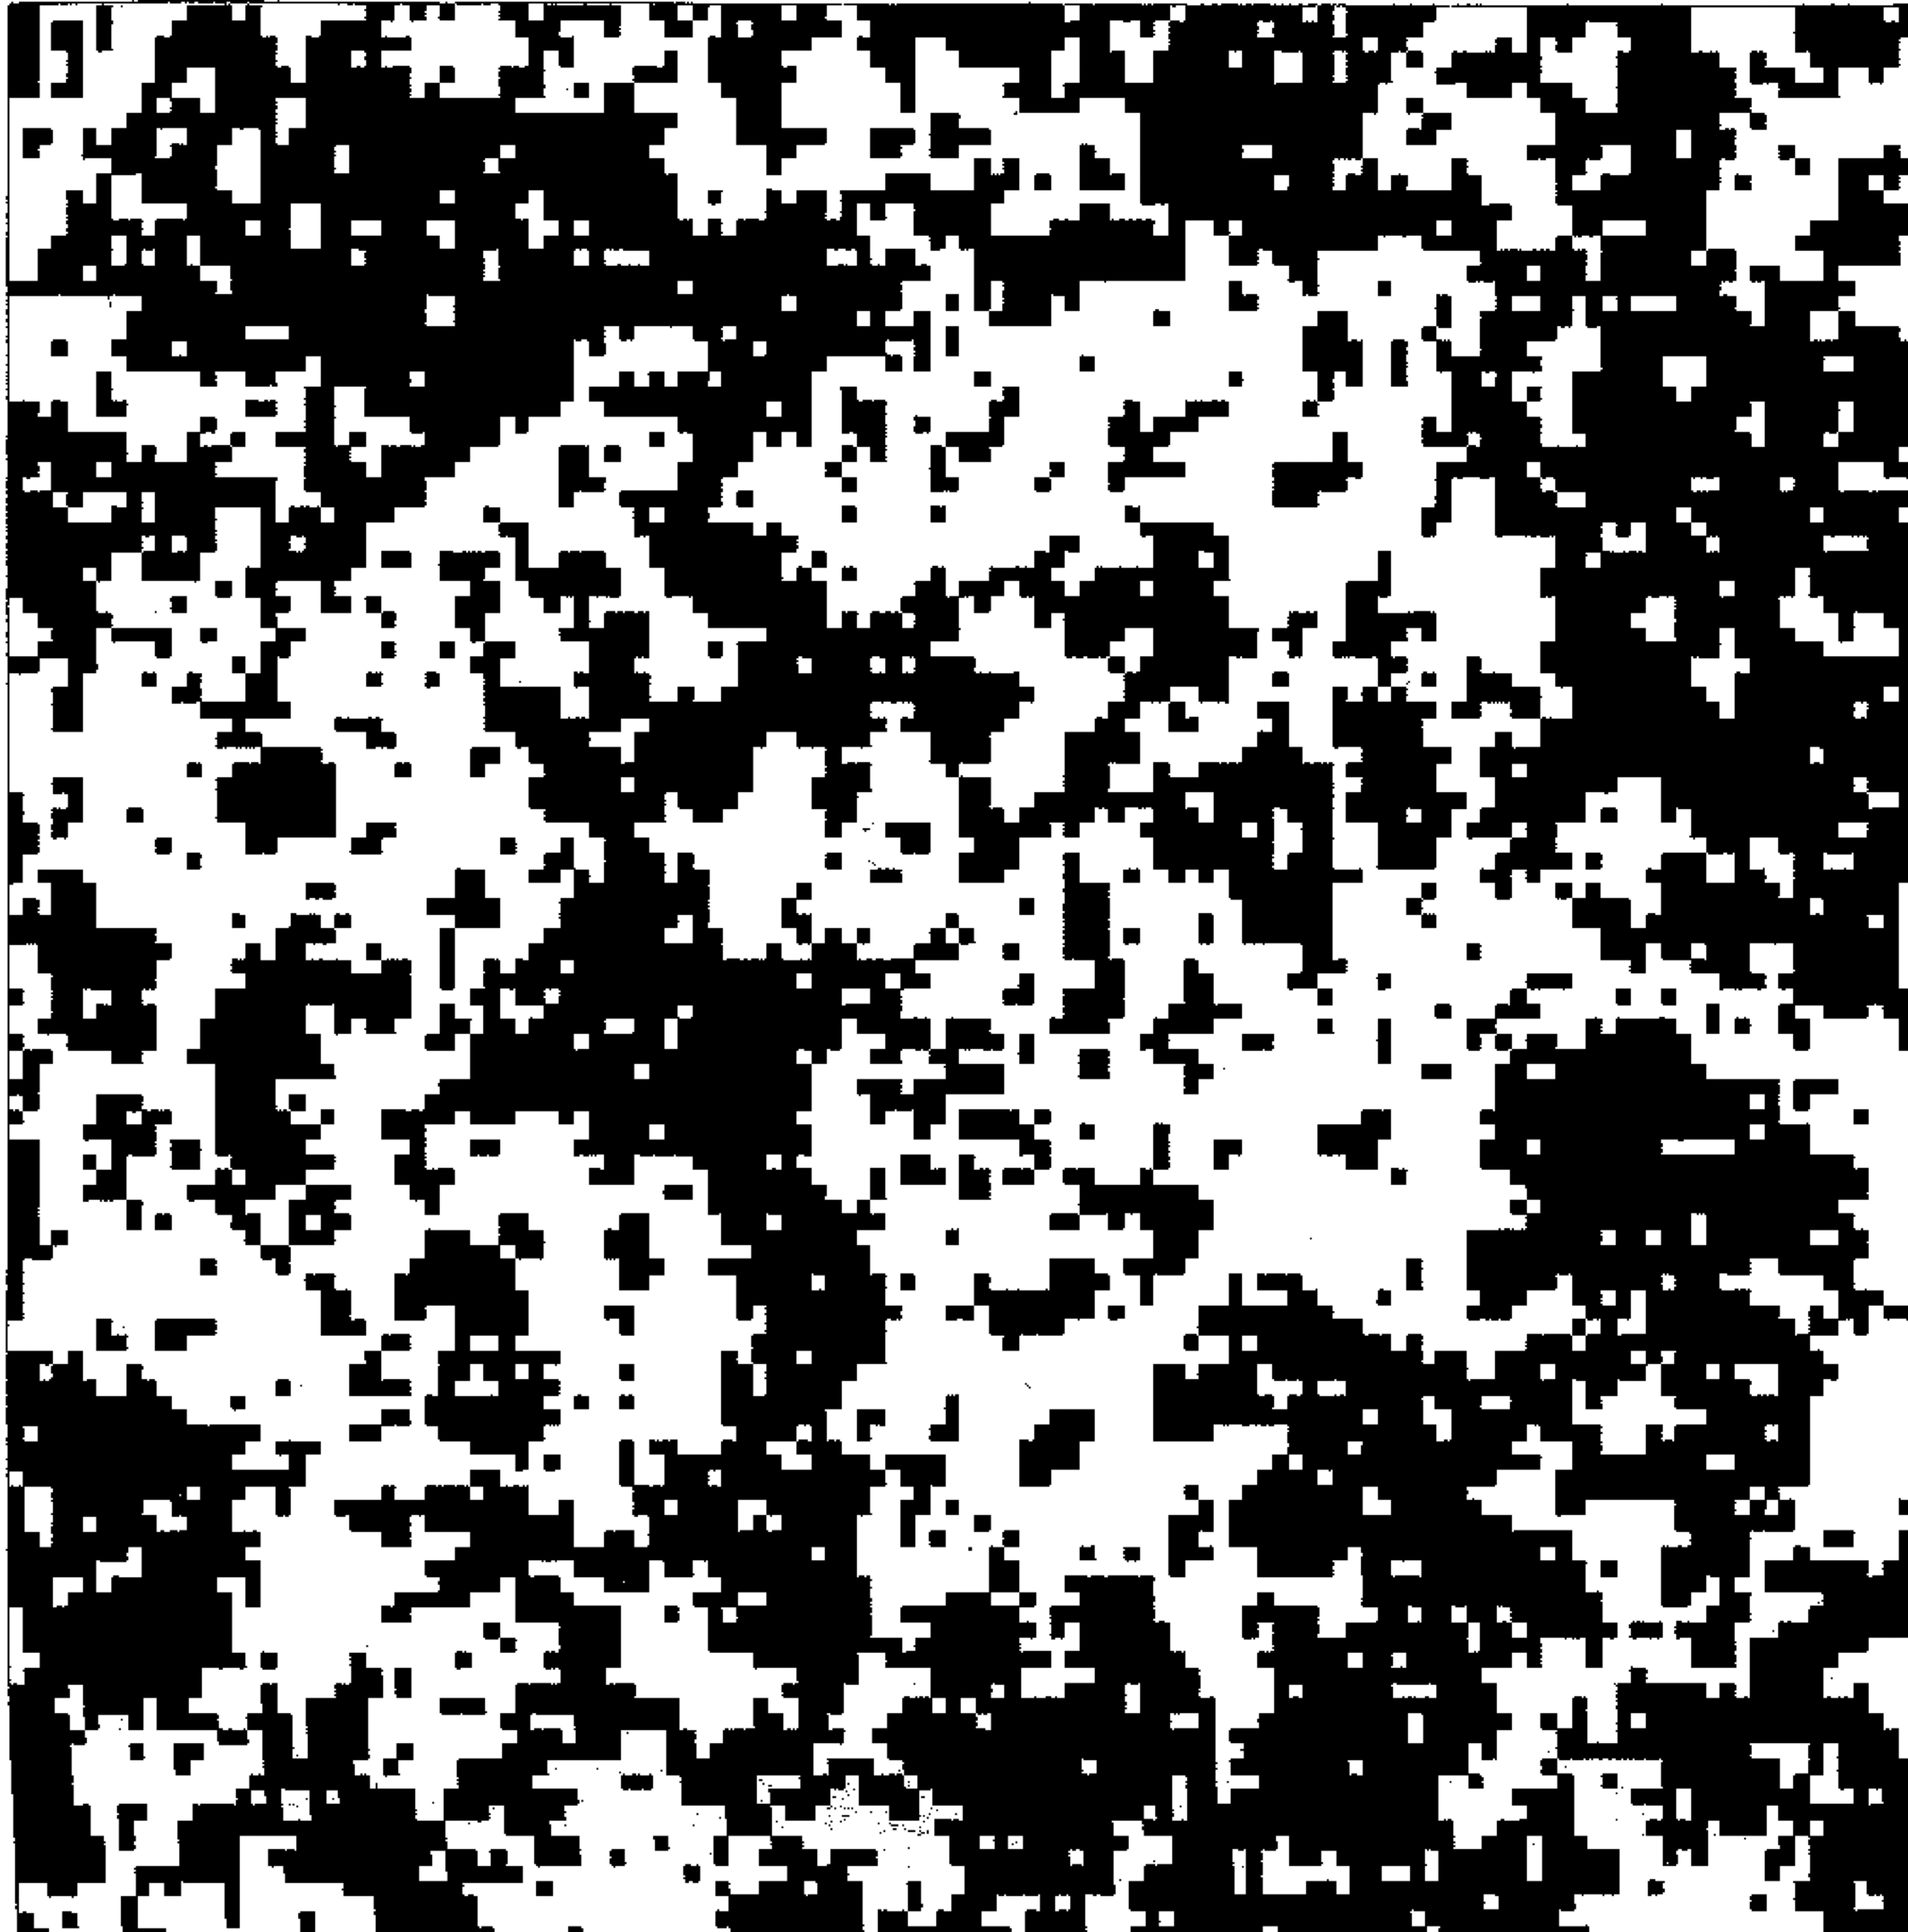
\includegraphics[keepaspectratio]{phase-transitions/Figs/supercrit.png}}

\subcaption{\label{}\(T=1.2T_c\)}
\end{minipage}%
%
\begin{minipage}{0.33\linewidth}

\pandocbounded{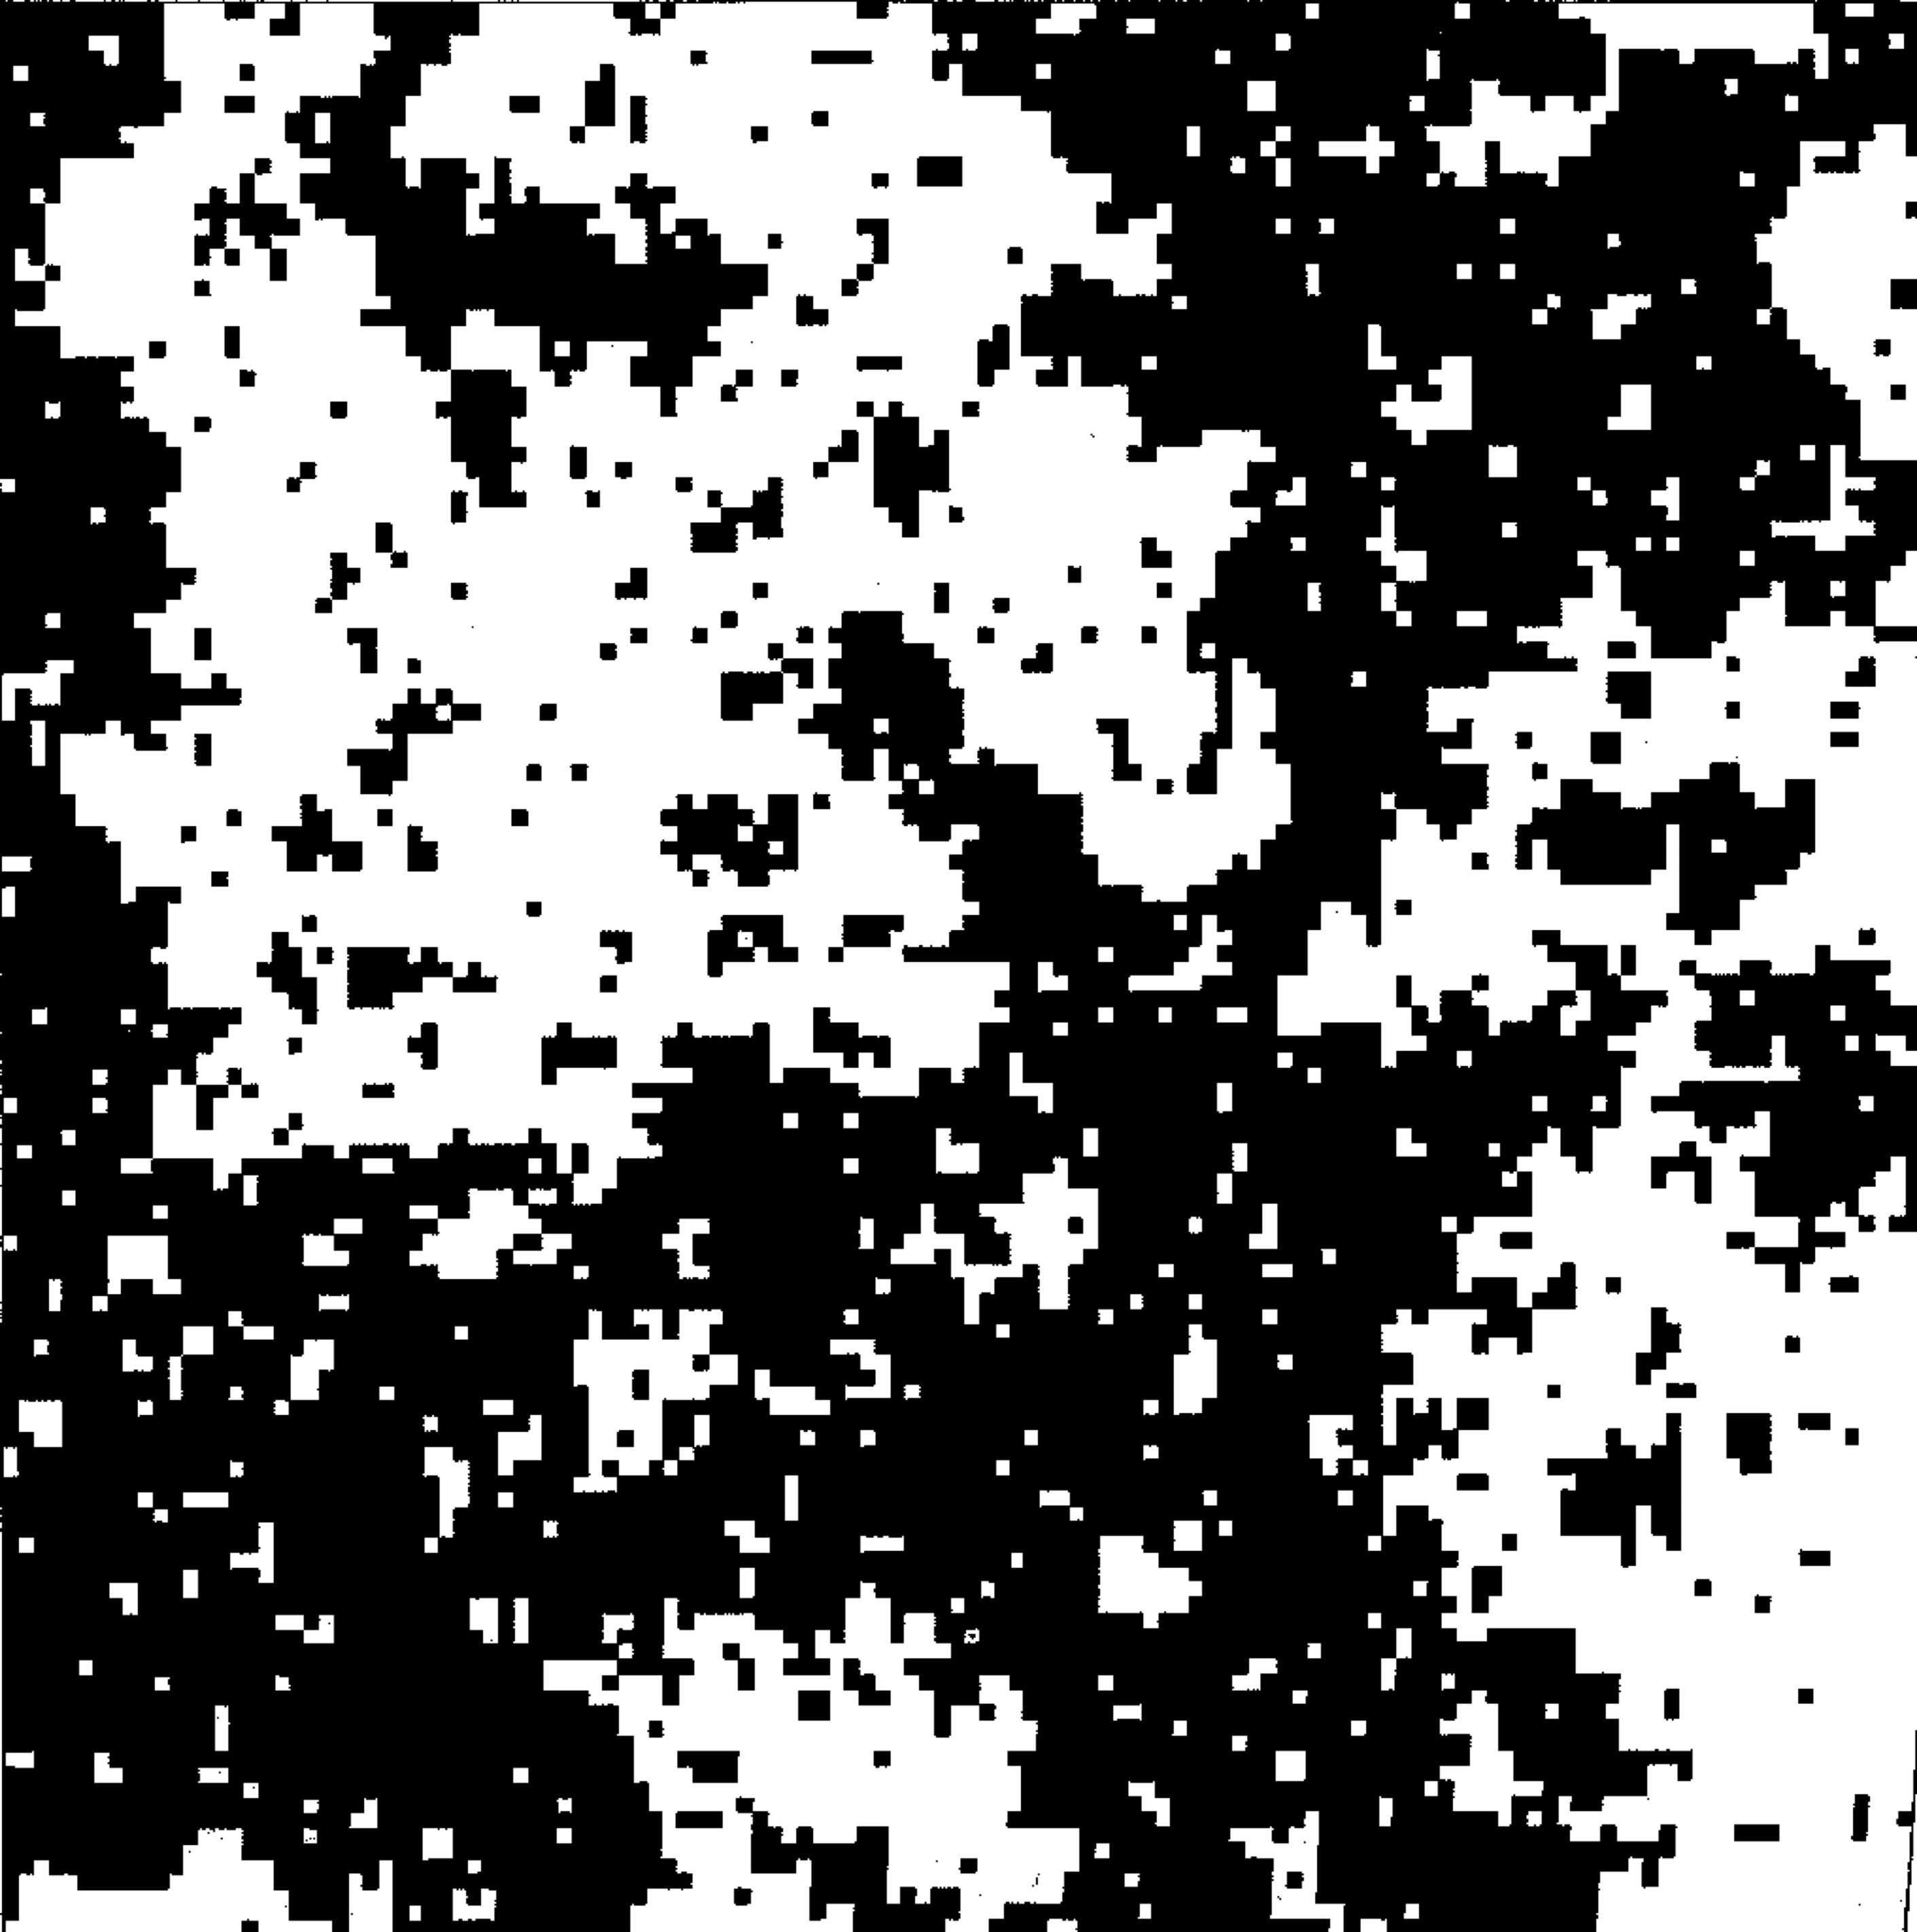
\includegraphics[keepaspectratio]{phase-transitions/Figs/crit.png}}

\subcaption{\label{}\(T=T_c\)}
\end{minipage}%
%
\begin{minipage}{0.33\linewidth}

\pandocbounded{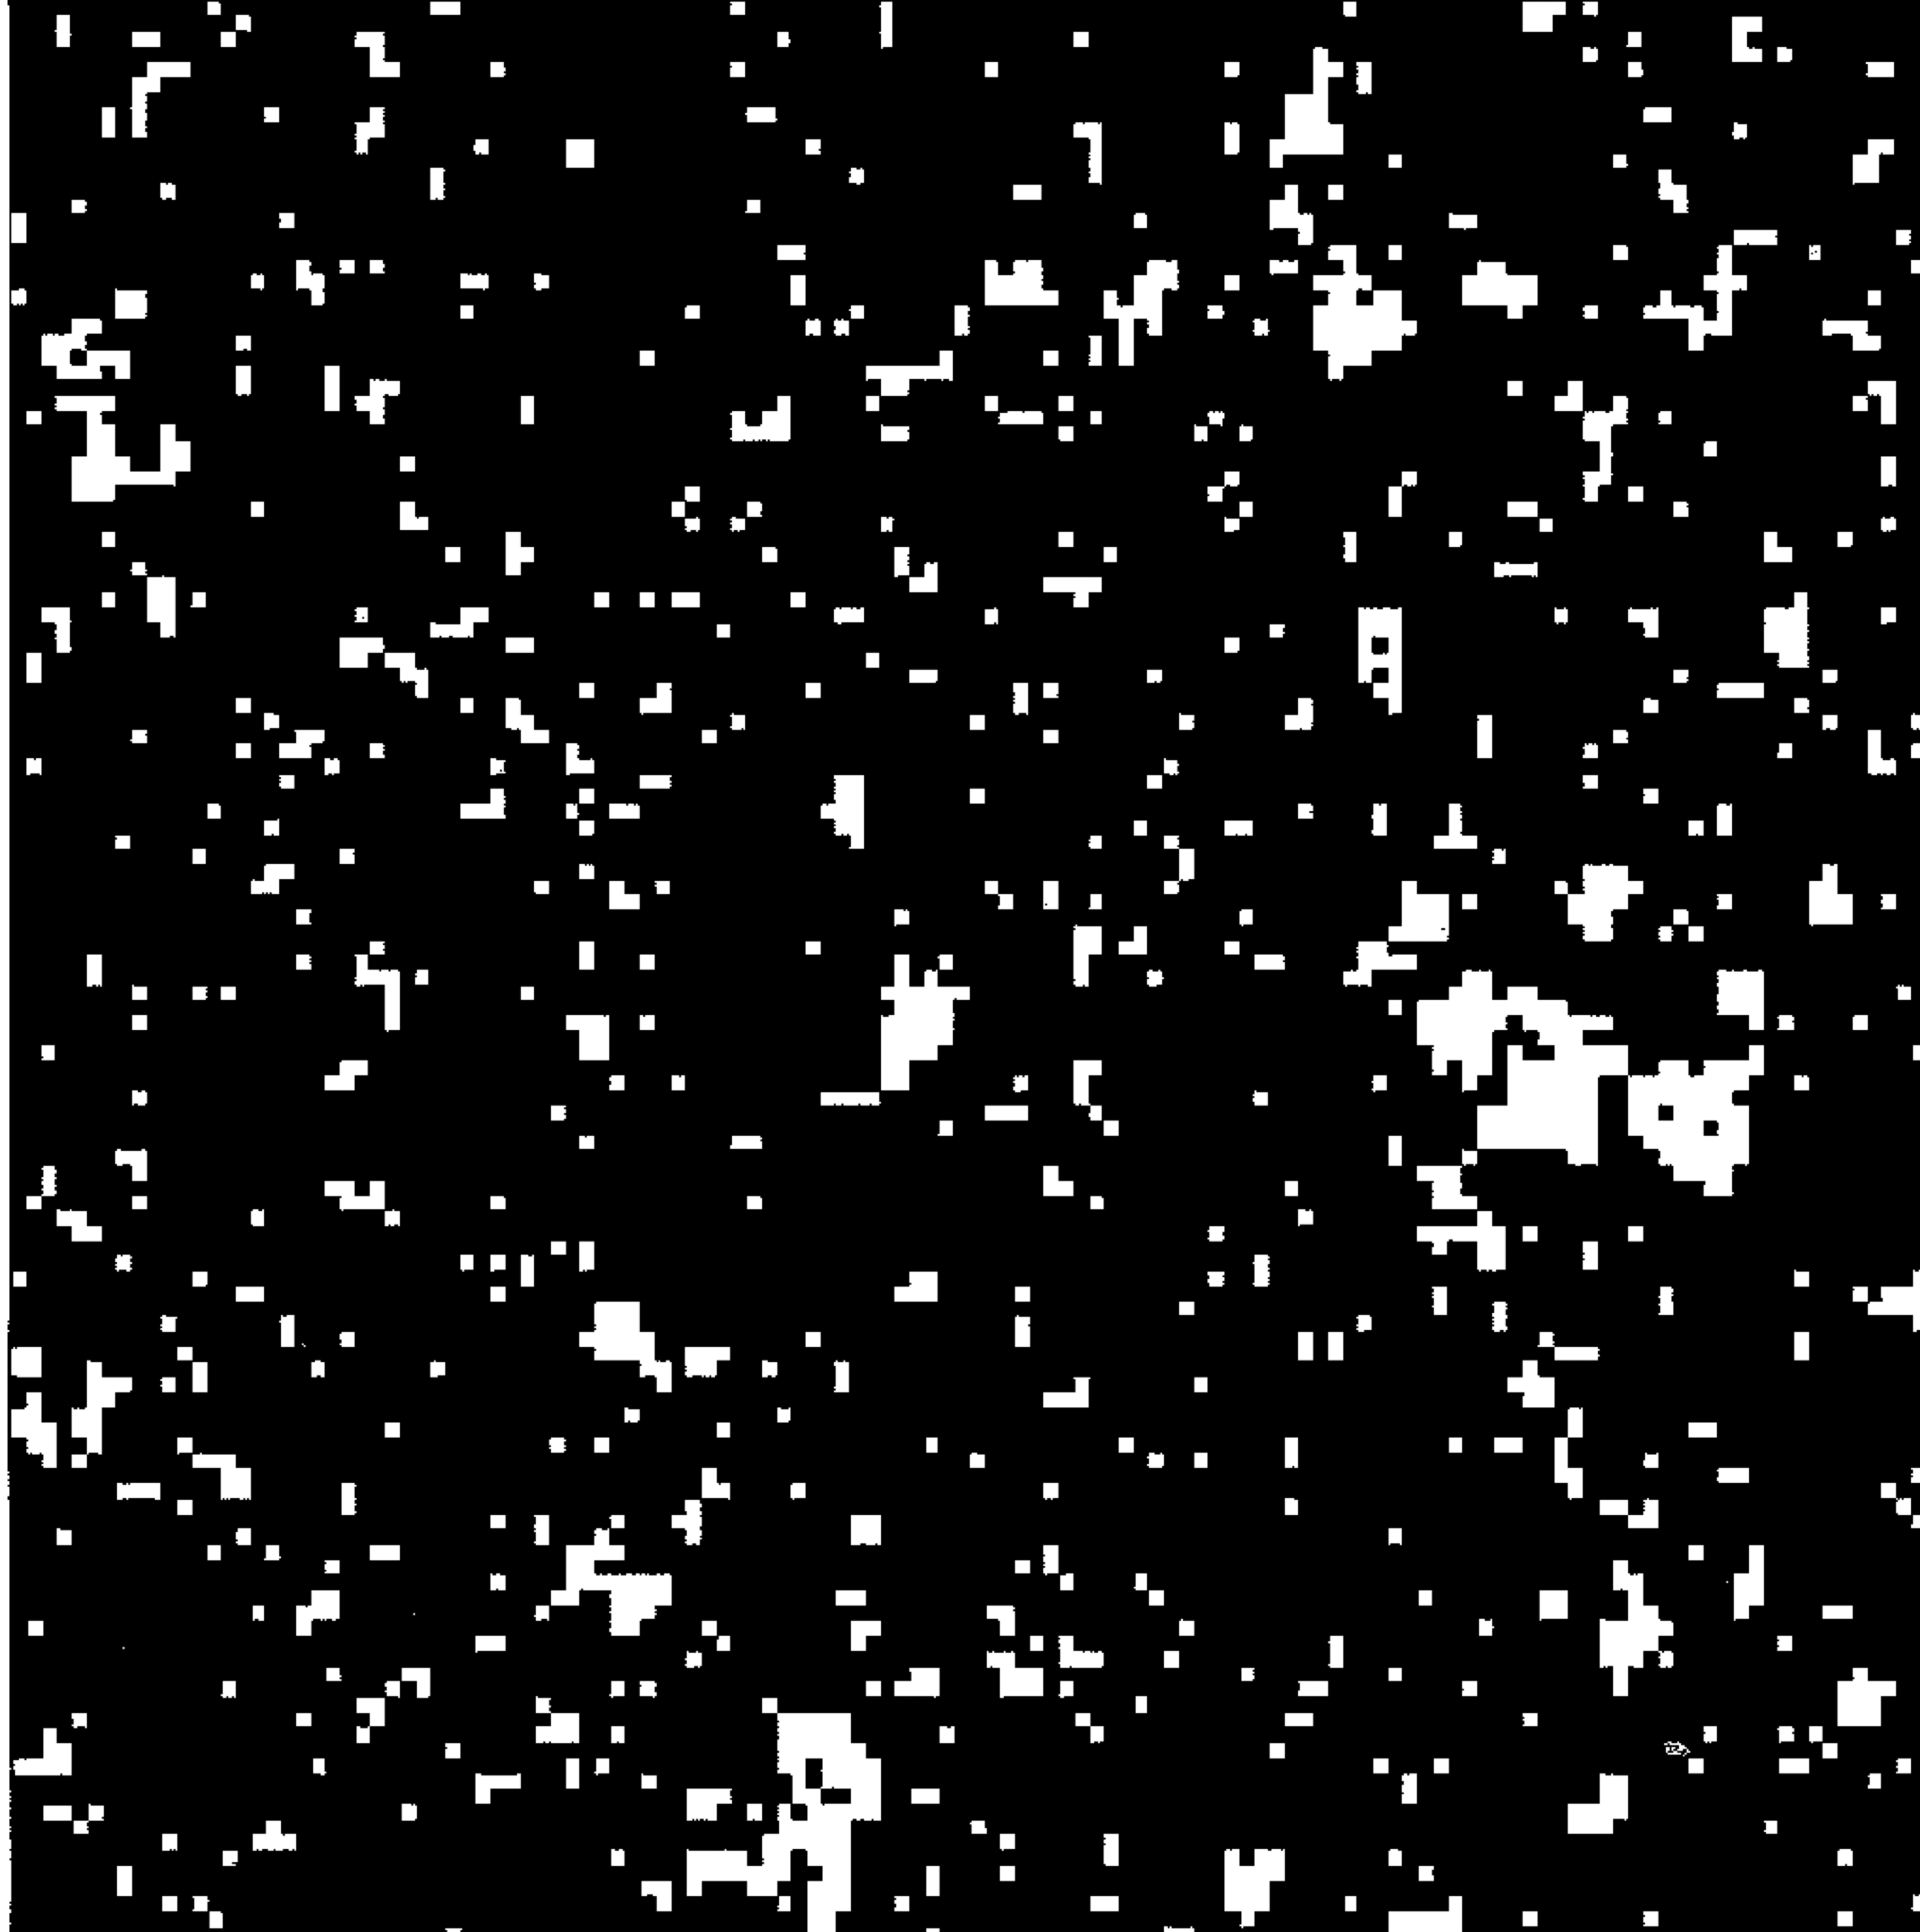
\includegraphics[keepaspectratio]{phase-transitions/Figs/subcrit.png}}

\subcaption{\label{}\(T=0.95T_c\)}
\end{minipage}%

\caption{\label{fig-snapshots}Configurations of the 2d Ising model. The
patterns depict typical arrangements of the spins (white=+1, black=−1)
generated in a computer simulation of the Ising model on a square
lattice of \(N=512\) sites, at temperatures (from left to right) of
\(T= 1.2T_c\), \(T=T_c\), and \(T=0.95T_c\). In each case only a portion
of the system containing \(128\) sites in shown. The typical island size
is a measure of the correlation length \(\xi\): the excess of black over
white (below \(T_c\) is a measure of the order parameter.}

\end{figure}%

\href{https://physics.weber.edu/schroeder/software/demos/isingmodel.html}{An
interactive Monte Carlo simulation of the Ising model} demonstrates the
phenomenology, By altering the temperature you will be able to observe
for yourself how the spin arrangements change as one traverses the
critical region. Pay particular attention to the configurations near the
critical point. They have very interesting properties. We will return to
them later!

Although the 2-d Ising model may appear at first sight to be an
excessively simplistic portrayal of a real magnetic system, critical
point universality implies that many physical observables such as
critical exponents are not materially influenced by the actual nature of
the microscopic interactions. The Ising model therefore provides a
simple, yet \emph{quantitatively} accurate representation of the
critical properties of a whole range of real magnetic (and indeed fluid)
systems. This universal feature of the model is largely responsible for
its ubiquity in the field of critical phenomena. We shall explore these
ideas in more detail later in the course.

\section{Exact solutions: the one dimensional Ising
chain}\label{exact-solutions-the-one-dimensional-ising-chain}

One might well ask why the 2D Ising model is the simplest model to
exhibit a phase transition. What about the one-dimensional Ising model
(ie. spins on a line)? In fact in one dimension, the Ising model can be
solved exactly. It turns out that the system is paramagnetic for all
\(T>0\), so there is no phase transition at any finite temperature. To
see this, consider the ground state of the system in zero external
field. This will have all spins aligned the same way (say up), and hence
be ferromagnetic. Now consider a configuration with a various ``domain
walls'' dividing spin up and spin down regions:

\begin{figure}

\centering{

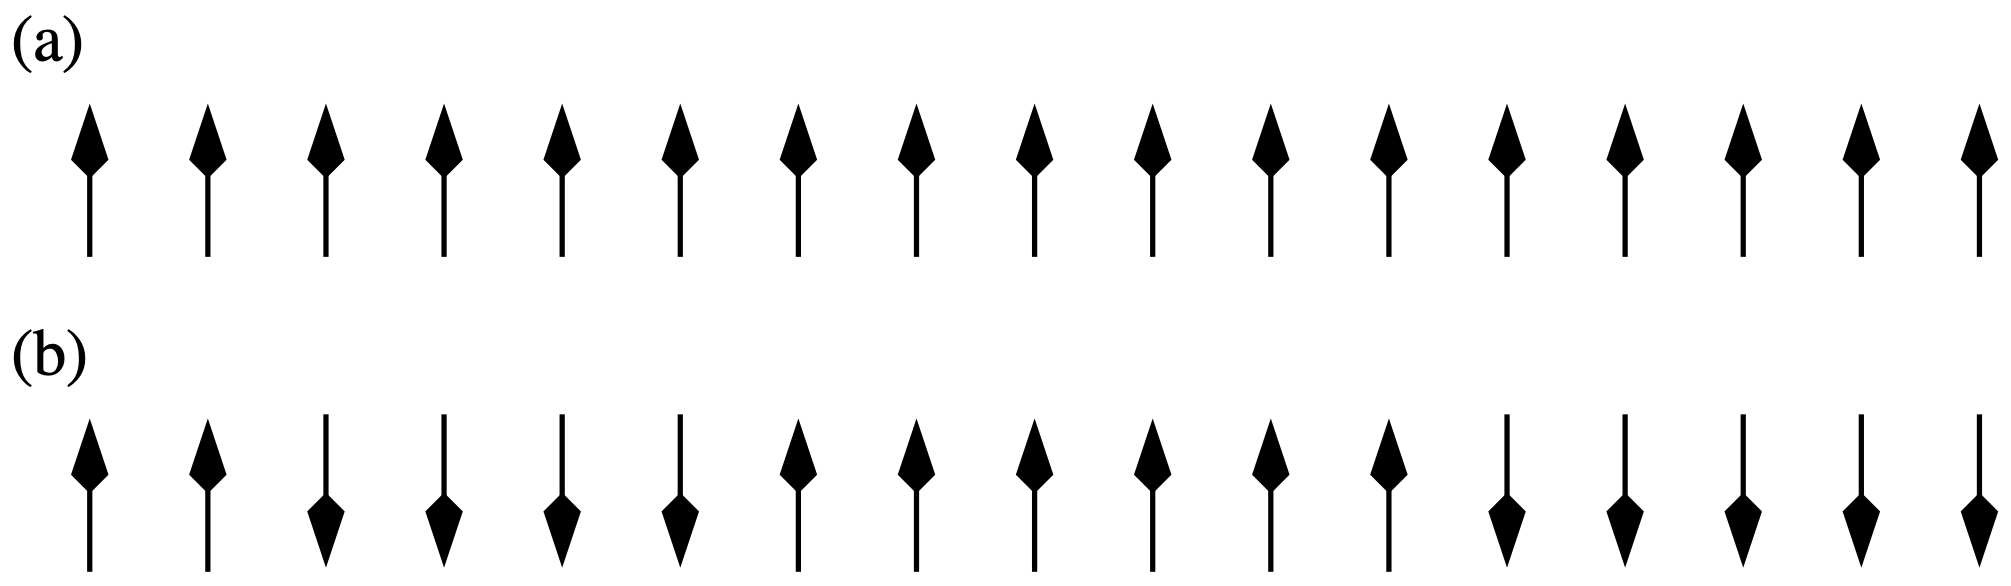
\includegraphics[width=0.8\linewidth,height=\textheight,keepaspectratio]{phase-transitions/Figs/chain.png}

}

\caption{\label{fig-isingchain}(a) Schematic of an Ising chain at
\(T=0\). (b) At a small finite temperature the chain is split into
domains of spins ordered in the same direction. Domains are separated by
notional domain ``walls'', which cost energy \(\Delta=2J\). Periodic
boundary conditions are assumed.}

\end{figure}%

Instead of considering the underlying spin configurations, we shall
describe the system in terms of the statistics of its domain walls. The
energy cost of a wall is \(\Delta = 2J\), independent of position.
Domain walls can occupy the bonds of the lattice, of which there are
\(N-1\). Moreover, the walls are noninteracting, except that you cannot
have two of them on the same bond. (Check through these ideas if you are
unsure.)

In this representation, the partition function involves a count over all
possible domain wall arrangements. Since the domain walls are non
interacting (eg it doesn't cost energy for one to move along the chain)
we can calculate \(Z\) by considering the partition function associated
with a single domain wall being present or absent on some given bond,
and then simply raise to the power of the number of bonds:

\[Z=Z_1^{N-1}\]

where

\[Z_1=e^{\beta J} + e^{\beta (J-\Delta)}=e^{\beta J}(1+e^{-\beta\Delta})\]
is the domain wall partition function for a single bond and represent
the sum over the two possible states: domain wall absent or present.
Then the free energy per bond of the system is

\[\beta f\equiv \beta F/(N-1)=-\ln Z_1=-\beta J-\ln(1+e^{-\beta\Delta})\]

The first term on the RHS is simply the energy per spin of the
ferromagnetic (ordered) phase, while the second term arises from the
free energy of domain walls. Clearly for any finite temperature (ie. for
\(\beta<\infty\)), this second term is finite and negative. Hence the
free energy will always be lowered by having a finite concentration of
domain walls in the system. Since these domain walls disorder the
system, leading to a zero average magnetisation, the 1D system is
paramagnetic for all finite temperatures. \emph{Exercise}: Explain why
this argument works only in 1D.

The animation below lets you see qualitatively how the typical number of
domain walls varies with temperature. If you'd lke to explore more
quantitatively, a python code performing a Monte Carlo simulation is
available. You will learn about Monte Carlo simulation in the coursework
and in later parts of the course.

\begin{Shaded}
\begin{Highlighting}[]
\CommentTok{\#Monte Carlo simulation of the 1d Ising chain with periodic bounary conditions}
\ImportTok{import}\NormalTok{ numpy }\ImportTok{as}\NormalTok{ np}
\ImportTok{import}\NormalTok{ matplotlib.pyplot }\ImportTok{as}\NormalTok{ plt}
\ImportTok{from}\NormalTok{ matplotlib.animation }\ImportTok{import}\NormalTok{ FuncAnimation}
\ImportTok{from}\NormalTok{ matplotlib.widgets }\ImportTok{import}\NormalTok{ Slider}

\CommentTok{\# Number of spins}
\NormalTok{N }\OperatorTok{=} \DecValTok{20} 

\CommentTok{\# Initialize spins (+1 or {-}1)}
\NormalTok{spins }\OperatorTok{=}\NormalTok{ np.random.choice([}\OperatorTok{{-}}\DecValTok{1}\NormalTok{, }\DecValTok{1}\NormalTok{], size}\OperatorTok{=}\NormalTok{N)}

\CommentTok{\# Initial temperature}
\NormalTok{T }\OperatorTok{=} \FloatTok{2.0}

\CommentTok{\# Set up figure and axis for the spins}
\NormalTok{fig, ax }\OperatorTok{=}\NormalTok{ plt.subplots(figsize}\OperatorTok{=}\NormalTok{(}\DecValTok{10}\NormalTok{, }\DecValTok{2}\NormalTok{))}
\NormalTok{plt.subplots\_adjust(bottom}\OperatorTok{=}\FloatTok{0.25}\NormalTok{)  }\CommentTok{\# make room for slider}
\NormalTok{ax.set\_xlim(}\OperatorTok{{-}}\FloatTok{0.5}\NormalTok{, N }\OperatorTok{{-}} \FloatTok{0.5}\NormalTok{)}
\NormalTok{ax.set\_ylim(}\OperatorTok{{-}}\DecValTok{1}\NormalTok{, }\DecValTok{1}\NormalTok{)}
\NormalTok{ax.axis(}\StringTok{\textquotesingle{}off\textquotesingle{}}\NormalTok{)}

\CommentTok{\# Create text objects for each spin}
\NormalTok{texts }\OperatorTok{=}\NormalTok{ []}
\ControlFlowTok{for}\NormalTok{ i }\KeywordTok{in} \BuiltInTok{range}\NormalTok{(N):}
\NormalTok{    arrow }\OperatorTok{=} \StringTok{\textquotesingle{}↑\textquotesingle{}} \ControlFlowTok{if}\NormalTok{ spins[i] }\OperatorTok{==} \DecValTok{1} \ControlFlowTok{else} \StringTok{\textquotesingle{}↓\textquotesingle{}}
\NormalTok{    t }\OperatorTok{=}\NormalTok{ ax.text(i, }\DecValTok{0}\NormalTok{, arrow, fontsize}\OperatorTok{=}\DecValTok{24}\NormalTok{, ha}\OperatorTok{=}\StringTok{\textquotesingle{}center\textquotesingle{}}\NormalTok{, va}\OperatorTok{=}\StringTok{\textquotesingle{}center\textquotesingle{}}\NormalTok{)}
\NormalTok{    texts.append(t)}

\KeywordTok{def}\NormalTok{ update(frame):}
    \CommentTok{"""Perform Metropolis updates over all spins, then refresh display."""}
    \KeywordTok{global}\NormalTok{ spins, T}
    \ControlFlowTok{for}\NormalTok{ \_ }\KeywordTok{in} \BuiltInTok{range}\NormalTok{(N):}
\NormalTok{        i }\OperatorTok{=}\NormalTok{ np.random.randint(N)}
\NormalTok{        left }\OperatorTok{=}\NormalTok{ spins[(i }\OperatorTok{{-}} \DecValTok{1}\NormalTok{) }\OperatorTok{\%}\NormalTok{ N]}
\NormalTok{        right }\OperatorTok{=}\NormalTok{ spins[(i }\OperatorTok{+} \DecValTok{1}\NormalTok{) }\OperatorTok{\%}\NormalTok{ N]}
\NormalTok{        deltaE }\OperatorTok{=} \DecValTok{2} \OperatorTok{*}\NormalTok{ spins[i] }\OperatorTok{*}\NormalTok{ (left }\OperatorTok{+}\NormalTok{ right)}
        \CommentTok{\# Metropolis criterion ensures configurations appear with the correct Boltzmann probability}
        \ControlFlowTok{if}\NormalTok{ deltaE }\OperatorTok{\textless{}} \DecValTok{0} \KeywordTok{or}\NormalTok{ np.random.rand() }\OperatorTok{\textless{}}\NormalTok{ np.exp(}\OperatorTok{{-}}\NormalTok{deltaE }\OperatorTok{/}\NormalTok{ T):}
\NormalTok{            spins[i] }\OperatorTok{*=} \OperatorTok{{-}}\DecValTok{1}
    \CommentTok{\# Update arrows on screen}
    \ControlFlowTok{for}\NormalTok{ idx, t }\KeywordTok{in} \BuiltInTok{enumerate}\NormalTok{(texts):}
\NormalTok{        t.set\_text(}\StringTok{\textquotesingle{}↑\textquotesingle{}} \ControlFlowTok{if}\NormalTok{ spins[idx] }\OperatorTok{==} \DecValTok{1} \ControlFlowTok{else} \StringTok{\textquotesingle{}↓\textquotesingle{}}\NormalTok{)}
    \ControlFlowTok{return}\NormalTok{ texts}

\CommentTok{\# Create the animation with caching disabled and blit turned off}
\NormalTok{ani }\OperatorTok{=}\NormalTok{ FuncAnimation(}
\NormalTok{    fig,}
\NormalTok{    update,}
\NormalTok{    interval}\OperatorTok{=}\DecValTok{200}\NormalTok{,}
\NormalTok{    blit}\OperatorTok{=}\VariableTok{False}\NormalTok{,}
\NormalTok{    cache\_frame\_data}\OperatorTok{=}\VariableTok{False}
\NormalTok{)}

\CommentTok{\# Add a temperature slider}
\NormalTok{ax\_T }\OperatorTok{=}\NormalTok{ plt.axes([}\FloatTok{0.2}\NormalTok{, }\FloatTok{0.1}\NormalTok{, }\FloatTok{0.6}\NormalTok{, }\FloatTok{0.03}\NormalTok{], facecolor}\OperatorTok{=}\StringTok{\textquotesingle{}lightgray\textquotesingle{}}\NormalTok{)}
\NormalTok{slider\_T }\OperatorTok{=}\NormalTok{ Slider(ax\_T, }\StringTok{\textquotesingle{}Temperature T\textquotesingle{}}\NormalTok{, }\FloatTok{0.1}\NormalTok{, }\FloatTok{5.0}\NormalTok{, valinit}\OperatorTok{=}\NormalTok{T)}

\KeywordTok{def}\NormalTok{ on\_T\_change(val):}
    \CommentTok{"""Callback to update T when the slider changes."""}
    \KeywordTok{global}\NormalTok{ T}
\NormalTok{    T }\OperatorTok{=}\NormalTok{ val}

\NormalTok{slider\_T.on\_changed(on\_T\_change)}

\CommentTok{\# Show the plot (ani is kept in scope so it won\textquotesingle{}t be deleted)}
\NormalTok{plt.show()}
\end{Highlighting}
\end{Shaded}

\phantomsection\label{ising}

Temperature T =

2.0

\subsection{More general 1D spins systems: transfer matrix
method}\label{more-general-1d-spins-systems-transfer-matrix-method}

Generally speaking one-dimensional systems lend themselves to a degree
of analytic tractability not found in most higher dimensional models.
Indeed for the case of a 1-d assembly of \(N\) spins each having \(m\)
discrete energy states, and in the presence of a magnetic field, it is
possible to reduce the evaluation of the partition function to the
calculation of the eigenvalues of a matrix--the so called transfer
matrix.

Let us start by assuming that the assembly has cyclic boundary
conditions, then the total energy of configuration \(\{s\}\) is

\begin{aligned}
H(\{s\})=&-\sum_{i=1}^N (Js_is_{i+1}+Hs_i)\\
\:=&-\sum_{i=1}^N (Js_is_{i+1}+H(s_i+s_{i+1})/2)\\
\:=&\sum_{i=1}^N E(s_i,s_{i+1})
\end{aligned}

where we have defined \(E(s_i,s_{i+1})=-Js_is_{i+1}-H(s_i+s_{i+1})/2\).

Now the partition function may be written

\begin{equation}\phantomsection\label{eq-Vs}{\begin{aligned}
Z_N =& \sum_{\{s\}}\exp\left(-\beta H(\{s\})\right)\nonumber \\
 =&\sum_{\{s\}}\exp\left(-\beta[E(s_1,s_2)+E(s_2,s_3)+....E(s_N,s_1)]\right) \nonumber\\
 =&\sum_{\{s\}}\exp\left(-\beta E(s_1,s_2)\right)\exp\left(-\beta E(s_2,s_3)\right)....\exp\left(-\beta E(s_N,s_1)\right) \nonumber\\
=&\sum_{i,j,...,l=1}^m V_{ij}V_{jk}...V_{li} 
\end{aligned}}\end{equation}

where the \(V_{ij}=\exp(-\beta E_{ij})\) are elements of an
\(m \times m\) matrix \({\bf V}\), known as the transfer matrix
(\(i,j,k\) etc are dummy indices that run over the matrix elements). You
should see that the sum over the product of matrix elements picks up all
the terms in the partition function and therefore Equation~\ref{eq-Vs}
is an alternative way of writing the partition function.

The reason it is useful to transform to a matrix representation is that
it transpires that the sum over the product of matrix elements in
Equation~\ref{eq-Vs} is simply just the trace of \({\bf V}^N\) (check
this yourself for a short periodic chain), given by the sum of its
eigenvalues:-

\[Z_N=\lambda_1^N+\lambda_2^N+...\lambda_m^N\] For very large \(N\),
this expression simplifies further because the largest eigenvalue
\(\lambda_1\) dominates the behaviour since \((\lambda_2/\lambda_1)^N\)
vanishes as \(N\rightarrow \infty\). Consequently in the thermodynamic
limit one may put \(Z_N=\lambda_1^N\) and the problem reduces to
identifying the largest eigenvalue of the transfer matrix.

Specializing to the case of the simple Ising model in the presence of an
applied field \(H\), the transfer matrix takes the form

\[{\bf V}(H)=\left(
\begin{array}{cc}
e^{\beta(J+H)} & e^{-\beta J} \\
e^{-\beta J}   & e^{\beta(J-H)}
\end{array} \right)\]

This matrix has two eigenvalues which can be readily calculated in the
usual fashion as the roots of the characteristic polynomial
\(|{\bf V}-\lambda{\bf I}|\). They are

\[\lambda_{\pm}=e^{\beta J}\cosh(\beta H) \pm \sqrt{e^{2\beta J}\sinh^2\beta H+e^{-2\beta J}}.\]

Hence the free energy per spin \(f=-k_BT\ln \lambda_+\) is

\[f=-k_BT\ln \left[e^{\beta J}\cosh(\beta H) + \sqrt{e^{2\beta J}\sinh^2\beta H+e^{-2\beta J}}\right].\]

The Ising model in 2D can also be solved exactly, as was done by Lars
Onsager in 1940. The solution is extremely complicated and is regarded
as one of the pinnacles of statistical mechanics. In 3D no exact
solution is known.

\chapter{Mean field theory and perturbation
schemes}\label{mean-field-theory-and-perturbation-schemes}

Of the wide variety of models of interest to the critical point
theorist, the majority have shown themselves intractable to direct
analytic (pen and paper) assault. In a very limited number of instances
models have been solved exactly, yielding the phase coexistence
parameters, critical exponents and the critical temperature. The 2-d
spin-\(\frac{1}{2}\) Ising model is certainly the most celebrated such
example, its principal critical exponents are found to be
\(\beta=\frac{1}{8}, \nu=1, \gamma=\frac{7}{4}\). Its critical
temperature is \(-2J/\ln(\sqrt{2}-1)\approx 2.269J\). Unfortunately such
solutions rarely afford deep insight to the general framework of
criticality although they do act as an invaluable test-bed for new and
existing theories.

The inability to solve many models exactly often means that one must
resort to approximations. One such approximation scheme is mean field
theory.

\section{Mean field solution of the Ising model}\label{sec:mfising}

Let us look for a mean field expression for the free energy of the Ising
model whose Hamiltonian is given in Equation~\ref{eq-ising} . Write

\[s_i=\langle s_i\rangle+(s_i-\langle s_i\rangle)=m+(s_i-m)=m+\delta s_i\]

Then \begin{equation}\phantomsection\label{eq-mfa}{\begin{aligned}
{\cal H}_I=&-J\sum_{<i,j>}[m+(s_i-m)][m+(s_j-m)]-H\sum_i s_i\nonumber\\
=&-J\sum_{<i,j>}[m^2+m(s_i-m)+m(s_j-m)+\delta s_i\delta s_j]-H\sum_i s_i\nonumber\\
=&-J\sum_{i}(qms_i-qm^2/2)-H\sum_i s_i-J\sum_{<i,j>}\delta s_i\delta s_j 
\end{aligned}}\end{equation} where in the last line we have used the
fact that when for each site \(i\) we perform the sum \(\sum_{<i,j>}\)
over bonds of a quantity which is independent of \(s_j\), then the
result is just the number of bonds per site times that quantity. Since
the number of bonds on a lattice of \(N\) sites of coordination \(q\) is
\(Nq/2\) (because each bond is shared between two sites), there are
therefore \(q/2\) bonds per site.

Now the mean field approximation is to ignore the last term in the last
line of Equation~\ref{eq-mfa} giving the configurational energy as

\[
{\cal H}_{mf}=-\sum_{i}H_{mf}s_i+NqJm^2/2
\] with \(H_{mf}\equiv qJm+ H\) the ``mean field'' seen by spin \(s_i\).
As all the spins are decoupled (independent) in this approximation we
can write down the partition function, which follows by taking the
partition function for a single spin (by summing the Boltzmann factor
for \(s_i=\pm 1\)) and raising to the power \(N\) to find

\[
Z=e^{-\beta qJm^2N/2}[2\cosh(\beta(qJm+H))]^N
\]

The free energy follows as

\[F(m)=NJqm^2/2-Nk_BT\ln[2\cosh(\beta (qJm+H)]\:.\]

and the magnetisation as

\[
m=-\frac{1}{N}\frac{\partial F}{\partial H}=\tanh(\beta(qJm+H))
\]

To find \(m(H,T)\), we must numerically solve this last equation self
consistently.

Note that we can obtain \(m\) in a different way. Consider some arbitary
spin, \(s_i\) say. Then this spin has an energy \({\cal H}_{mf}(s_i)\).
Considering this energy for both cases \(s_i=\pm 1\) and the probability
\(p(s_i)=e^{-\beta{\cal H}_{mf}(s_i)}/Z\) of each, we have that

\[\langle s_i\rangle=\sum_{s_i=\pm 1}s_ip(s_i)\] but for consistancy,
\(\langle s_i\rangle=m\). Thus

\begin{equation}\phantomsection\label{eq-mfmag}{
\begin{aligned}
m & = \sum_{s_i=\pm 1}s_ip(s_i)\nonumber\\
 \: & = \frac{e^{\beta(qJm+H)}-e^{\beta(qJm+H)}} {e^{\beta(qJm+H)}+e^{-\beta(qJm+H)}}\nonumber\\
 \: & = \tanh(\beta(qJm+H))
\end{aligned}}\end{equation} as before.

\section{Spontaneous symmetry breaking}\label{sec-breaking}

\begin{figure}

\centering{

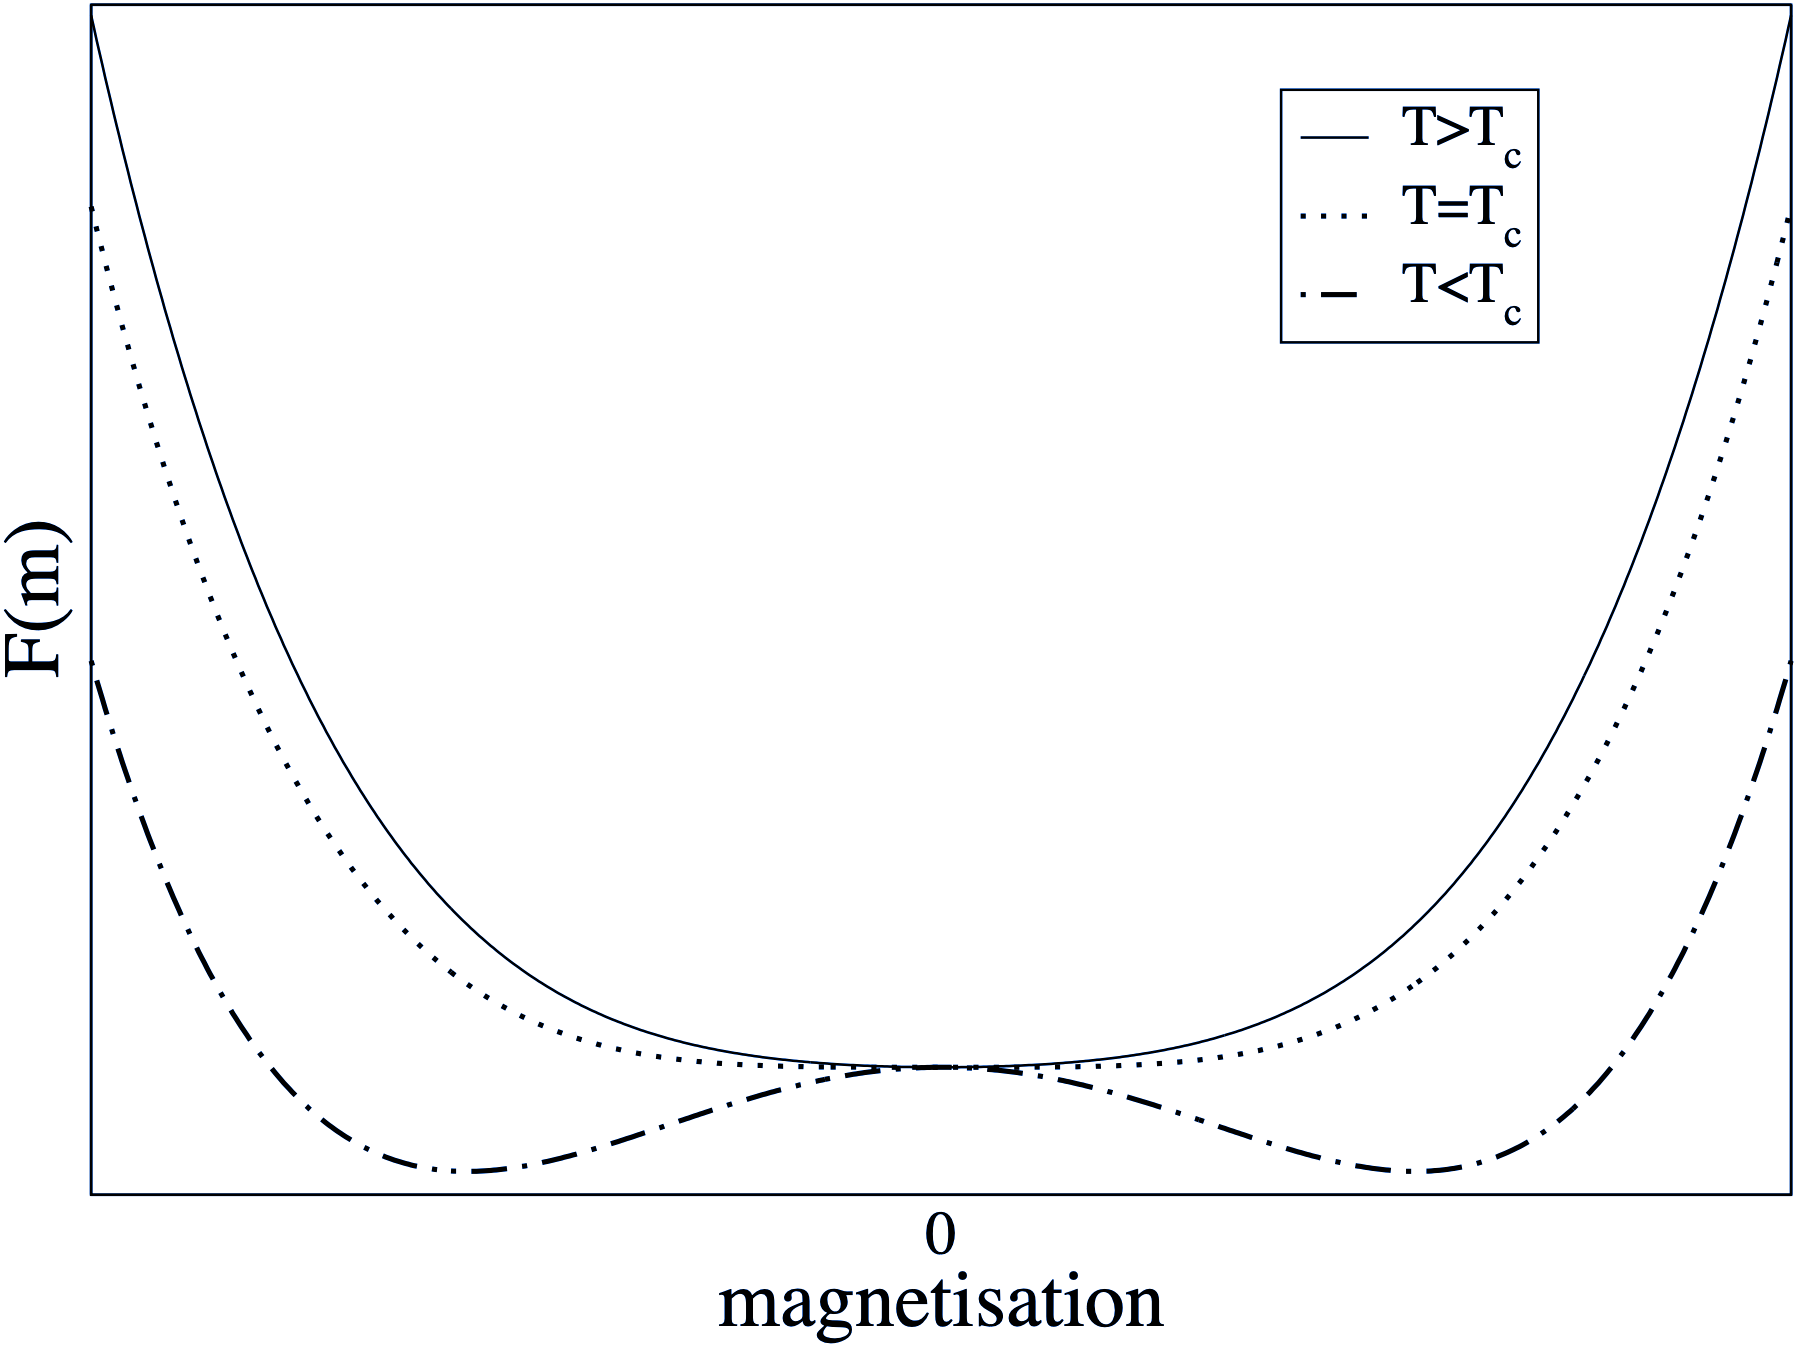
\includegraphics[width=0.7\linewidth,height=\textheight,keepaspectratio]{phase-transitions/Figs/freeenergy_color.png}

}

\caption{\label{fig-freeenergy}Schematic of the form of the free energy
for a critical, subcritical and supercritical temperature}

\end{figure}%

This mean field analysis reveals what is happening in the Ising model
near the critical temperature \(T_c\). Figure~\ref{fig-freeenergy} shows
sketches for \(\beta F(m)/N\) as a function of temperature, where for f
simplicity we restrict attention to \(H=0\). In this case \(F(m)\) is
symmetric in \(m\), Moreover, at high \(T\), the entropy dominates and
there is a single minimum in \(F(m)\) at \(m=0\). As \(T\) is lowered,
there comes a point (\(T=T_c=qJ/k_B\)) where the curvature of \(F(m)\)
at the origin changes sign; precisely at this point

\[\frac{\partial^2 F}{\partial m^2}=0.\] At lower temperature, there are
instead two minima at nonzero \(m=\pm m^\star\), where the
\emph{equilibrium magnetisation} \(m^\star\) is the positive root
(calculated explicitly below) of

\[m^\star=\tanh(\beta Jqm^\star)= \tanh(\frac{m^\star T_c}{T})\] The
point \(m=0\) which remains a root of this equation, is clearly an
unstable point for \(T<T_c\) (since \(F\) has a maximum there).

This is an example of spontaneous symmetry breaking. In the absence of
an external field, the Hamiltonian (and therefore the free energy) is
symmetric under \(m\to -m\). Accordingly, one might expect the actual
state of the system to also show this symmetry. This is true at high
temperature, but spontaneously breaks down at low ones. Instead there
are a pair of ferromagnetic states (spins mostly up, or spins mostly
down) which -- by symmetry-- have the same free energy, lower than the
unmagnetized state.

\section{Phase diagram}\label{phase-diagram}

The resulting zero-field magnetisation curve \(m(T,H=0)\) looks like
Figure~\ref{fig-isingmag}.

\begin{figure}

\centering{

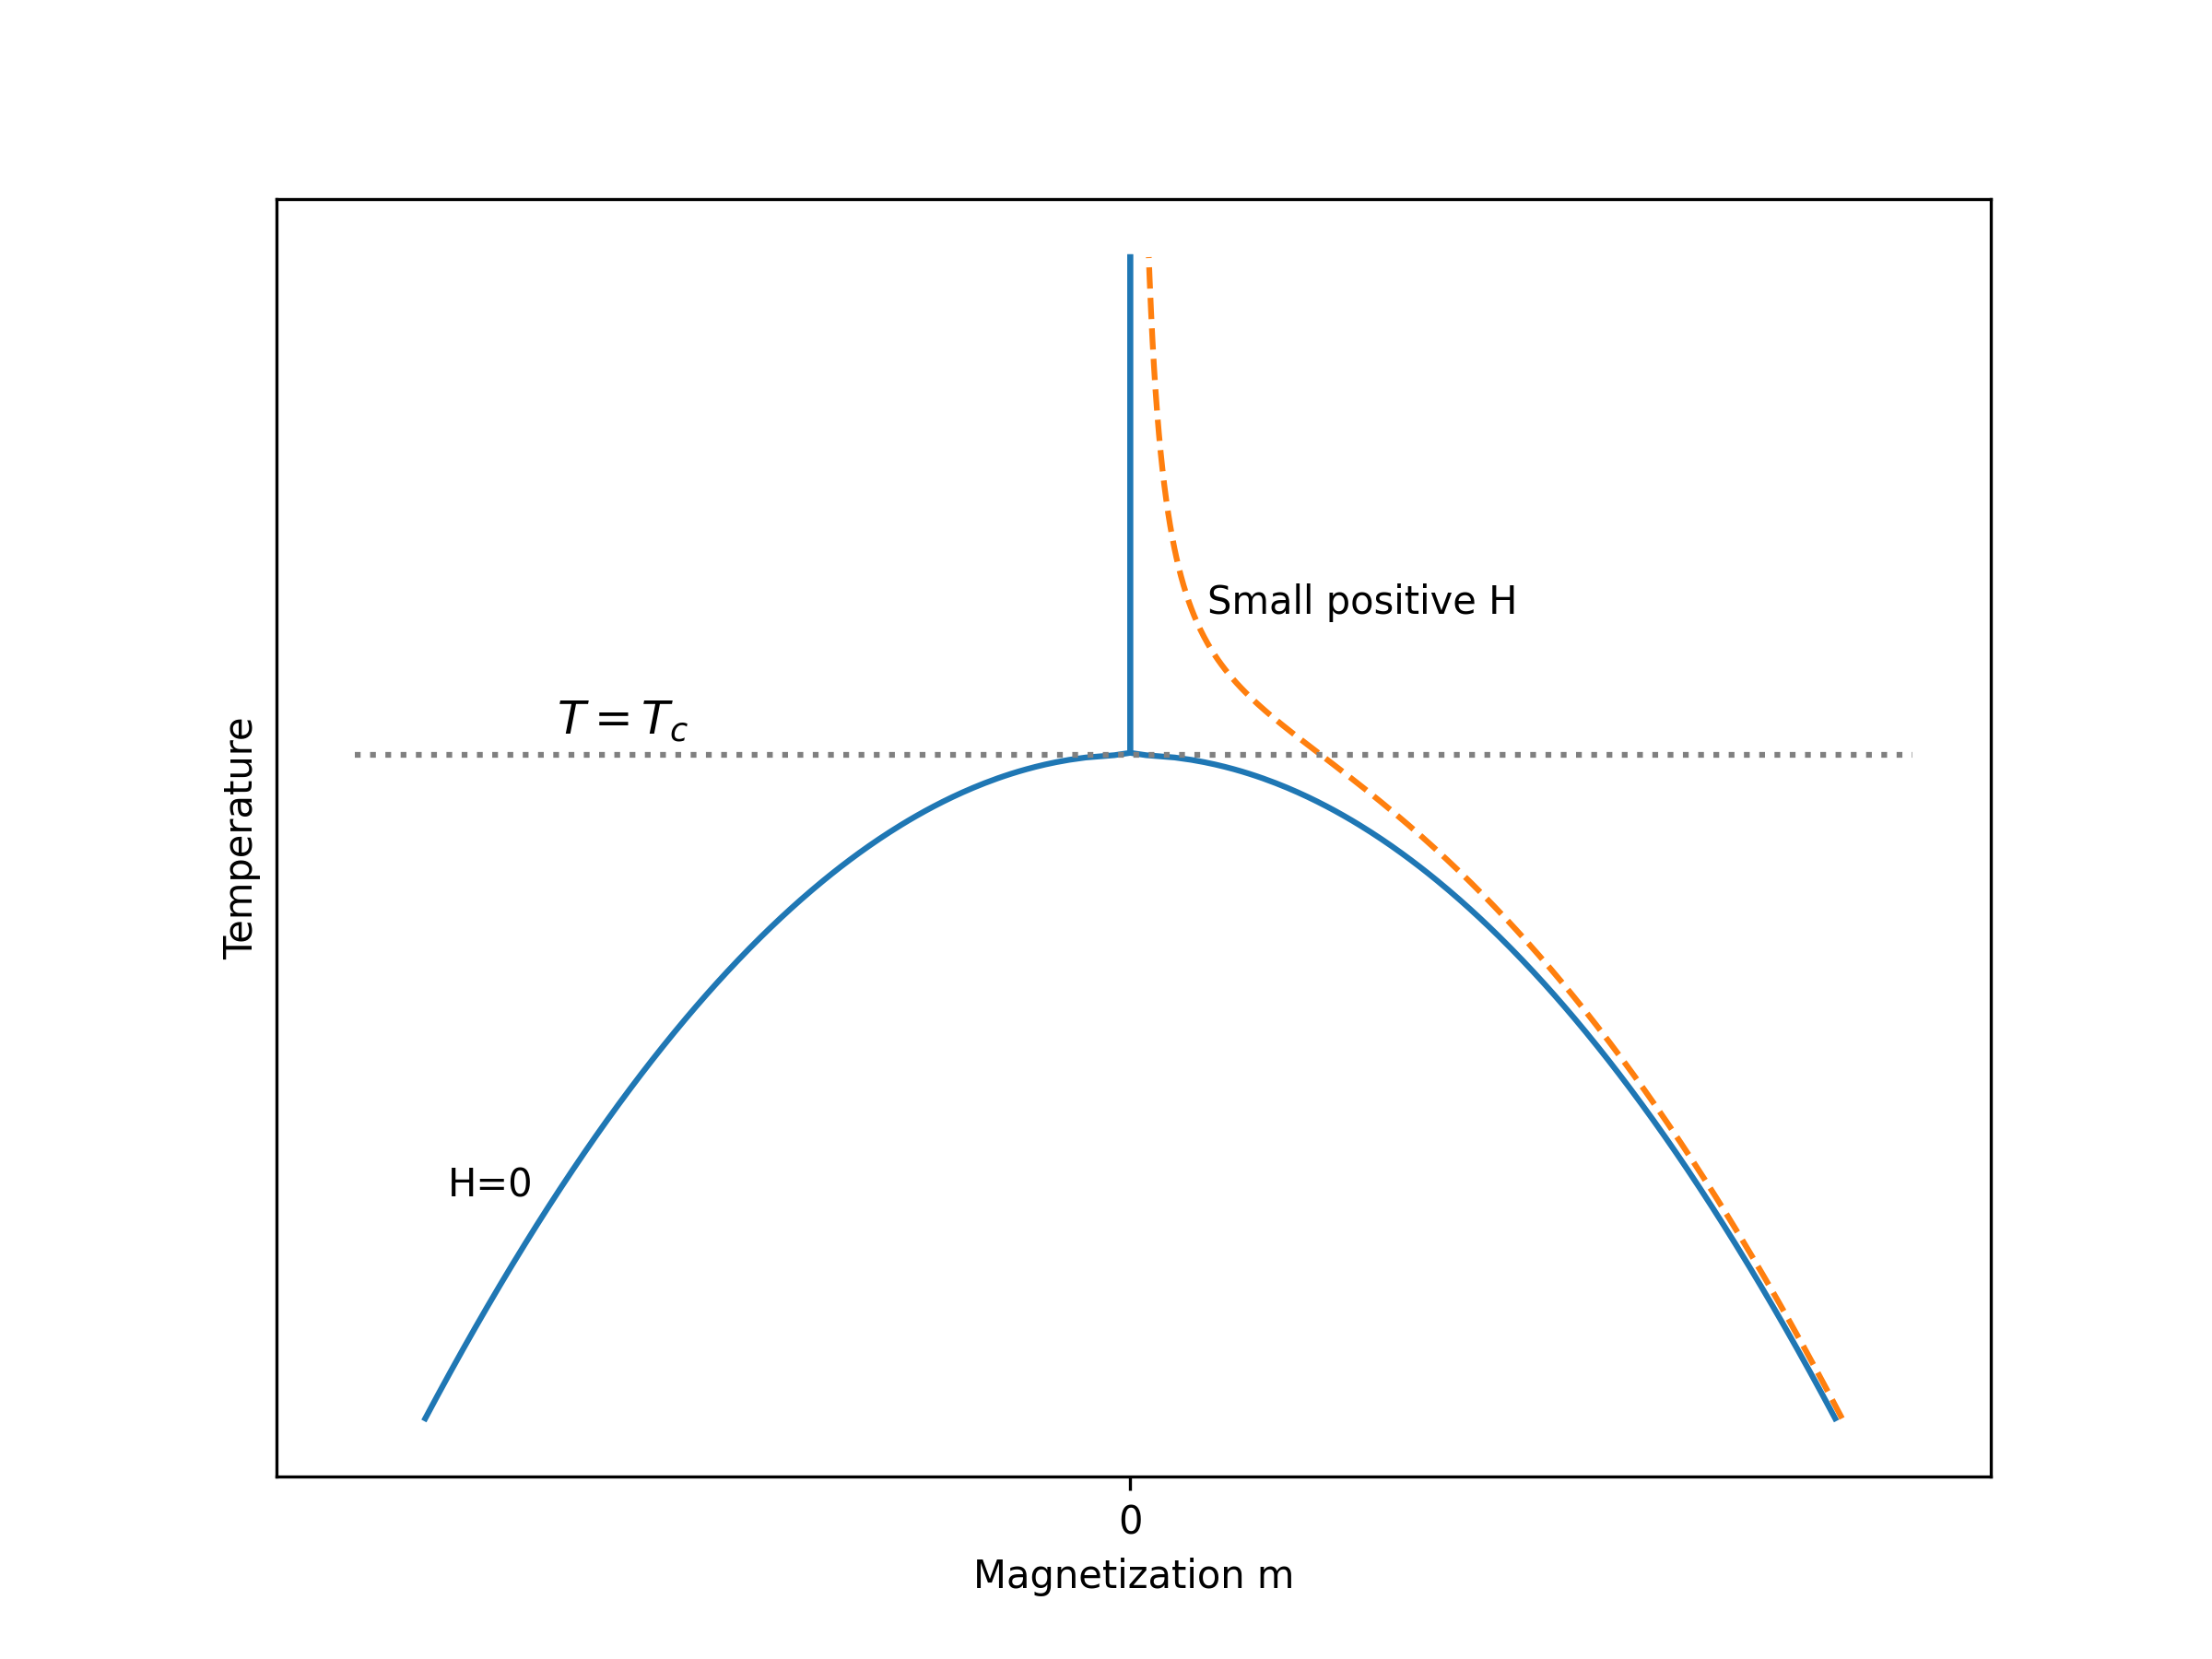
\includegraphics[width=0.7\linewidth,height=\textheight,keepaspectratio]{phase-transitions/Figs/isingmag_new.png}

}

\caption{\label{fig-isingmag}Phase diagram of a simple magnet in the
\(m\)-\(T\) plane.}

\end{figure}%

This shows the sudden change of behaviour at \(T_c\) (phase transition).
For \(T<T_c\) it is arbitrary which of the two roots \(\pm m^\star\) is
chosen; typically it will be different in different parts of the sample
(giving macroscopic ``magnetic domains''). But this behaviour with
temperature is \emph{qualitatively modified} by the presence of a field
\(H\), however small. In that case, there is always a slight
magnetization, even far above \(T_c\) and the curves becomes smoothed
out, as shown. There is no doubt which root will be chosen, and no
sudden change of the behaviour (no phase transition). Spontaneous
symmetry breaking does not occur, because the symmetry is already broken
by \(H\). (The curve \(F(m)\) is lopsided, rather than symmetrical about
\(m=0\).)

On the other hand, if we sit below \(T_c\) in a positive field (say) and
gradually reduce \(H\) through zero so that it becomes negative, there
is a \emph{very} sudden change of behaviour at \(h=0\): the equilibrium
state jumps discontinuously from \(m=m^\star\) to \(m=-m^\star\).

\begin{figure}

\centering{

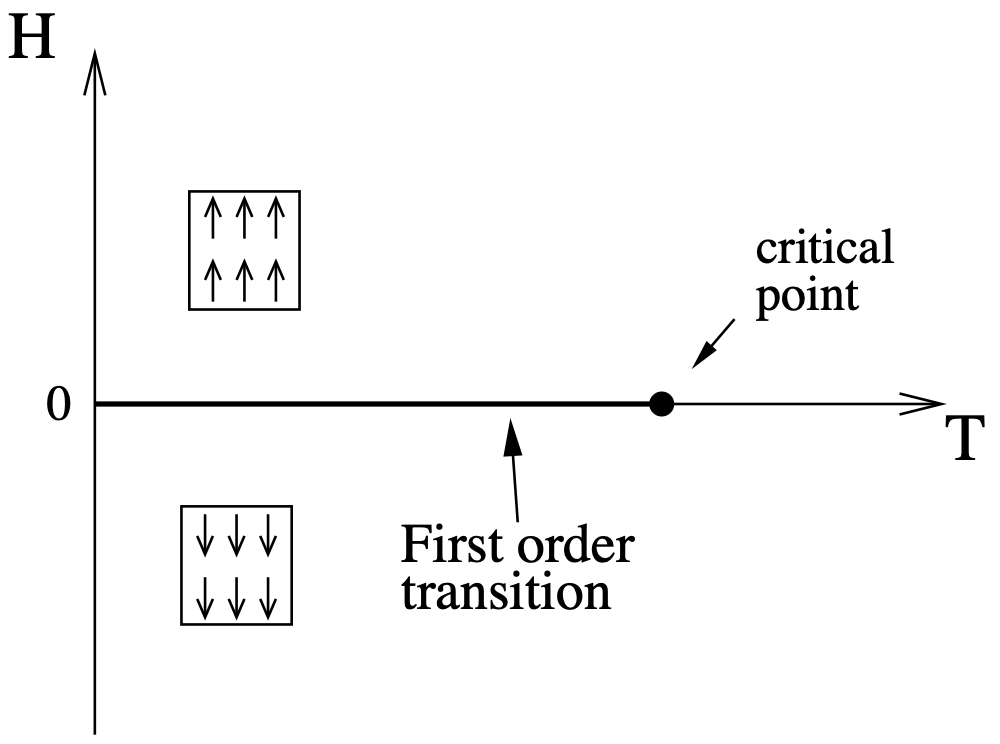
\includegraphics[width=0.7\linewidth,height=\textheight,keepaspectratio]{phase-transitions/Figs/isingpdH.png}

}

\caption{\label{fig-isingpdH}Phase diagram of a simple magnet in the
\(H\)-\(T\) plane.}

\end{figure}%

This is called a first order phase transition as opposed to the ``second
order'' or continuous transition that occurs at \(T_c\) in zero field.
The definitions are:

\emph{First order transition:} magnetisation (or similar order
parameter) depends discontinuously on a field variable (such as \(h\) or
\(T\)).

\emph{Continuous transition:} Change of functional form, but no
discontinuity in \(m\); typically, however,
\((\partial m/\partial T)_h\) (or similar) is either discontinuous, or
diverges with an integrable singularity.

In this terminology, we can say that the phase diagram of the magnet in
the \(H,T\) plane shows a line of first order phase transitions,
terminating at a continuous transition, which is the critical point.

\begin{tcolorbox}[enhanced jigsaw, leftrule=.75mm, bottomrule=.15mm, toprule=.15mm, colbacktitle=quarto-callout-caution-color!10!white, title=\textcolor{quarto-callout-caution-color}{\faFire}\hspace{0.5em}{Aside on Quantum Criticality}, breakable, titlerule=0mm, opacitybacktitle=0.6, colback=white, coltitle=black, colframe=quarto-callout-caution-color-frame, bottomtitle=1mm, rightrule=.15mm, toptitle=1mm, left=2mm, opacityback=0, arc=.35mm]

In some magnetic systems such as \(CePd_2Si_2\), one can, by applying
pressure or altering the chemical composition, depress the critical
temperature all the way to abolute zero! This may seem counterintuitive,
after all at \(T=0\) one should expect perfect ordering, not the large
fluctuations that accompany criticality. It turns out that the source of
the fluctuations that drive the system critical is zero point motion
associated with the Heisenberg uncertainty principle. Quantum
criticality is a matter of ongoing active research, and open questions
concern the nature of the phase diagrams and the relationship to
superconductivity. Although the subject goes beyond the scope of this
course, there is an accessible article
\href{https://arxiv.org/abs/1102.4628}{here} if you want to learn more.

\end{tcolorbox}

\section{A closer look: critical
exponents}\label{a-closer-look-critical-exponents}

Let us now see how we can calculate critical exponents within the mean
field approximation.

\subsection{Zero H solution and the order parameter
exponent}\label{zero-h-solution-and-the-order-parameter-exponent}

In zero field

\[m=\tanh(\frac{mT_c}{T})\] where \(T_c=qJ/k_B\) is the critical
temperature at which \(m\) first goes to zero.

We look for a solution where \(m\) is small (\(\ll 1\)). Expanding the
tanh function and replacing \(\beta=(k_BT)^{-1}\) yields

\[m=\frac{mT_c}{T}-\frac{1}{3}\left(\frac{mT_c}{T} \right)^3 +O(m^5)\:.\]
Then \(m=0\) is one solution. The other solution is given by

\[m^2=3\left(\frac{T}{T_c} \right)^3\left(\frac{T_c}{T} -1\right)\]

Now, considering temperatures close to \(T_c\) to guarantee small \(m\),
and employing the reduced temperature \(t=(T-T_c)/T_c\), one finds

\[m^2\simeq -3t\]

Hence

\begin{equation}\phantomsection\label{eq-mbeta}{\begin{aligned}
m= 0  &    ~~~\textrm{for } T>T_c \:\:\:  \textrm{ since~otherwise~{\it m}~imaginary}\nonumber\\
m= \pm\sqrt{-3t} & ~~\textrm{ for}  \:\:\: T<T_c ~~\textrm{ real}
\end{aligned} }\end{equation} This result implies that (within the mean
field approximation) the critical exponent \(\beta=1/2\).

\subsection{Finite (but small) field solution: the susceptibility
exponent}\label{sec:closerlook}

In a finite, but small field we can expand Equation~\ref{eq-mfmag} thus:

\[m=\frac{mT_c}{T}-\frac{1}{3}\left(\frac{mT_c}{T} \right)^3 +\frac{H}{kT}\]

Consider now the isothermal susceptibility

\begin{aligned}
\chi  \equiv & \left(\frac{\partial m}{\partial H}\right)_T\\
      =     & \frac{T_c}{T}\chi - \left(\frac{T_c}{T}\right)^3 \chi m^2 + \frac{1}{k_BT}  
\end{aligned}

Then

\[\chi \left[ 1-\frac{T_c}{T} +\left(\frac{T_c}{T}\right)^3m^2  \right]=\frac{1}{k_BT}\]

Hence near \(T_c\)

\[\chi=\frac{1}{k_BT_c}\left(\frac{1}{t+m^2}\right)\]

Then using the results of Equation~\ref{eq-mbeta}

\begin{aligned}
\chi= (k_BT_ct)^{-1} & \textrm{ for} ~~~ T> T_c \\
\chi= (-2k_BT_ct)^{-1} & \textrm{ for}  ~~~T \le T_c 
\end{aligned}

where one has to take the non-zero value for \(m\) below \(T_c\) to
ensure +ve \(\chi\), i.e.~thermodynamic stability. This result implies
that (within the mean field approximation) the critical exponent
\(\gamma=1\).

The schematic behaviour of the Ising order parameter and susceptibility
are shown in Figure~\ref{fig-mfsum}~(a) and (b)

\begin{figure}

\begin{minipage}{0.50\linewidth}

\centering{

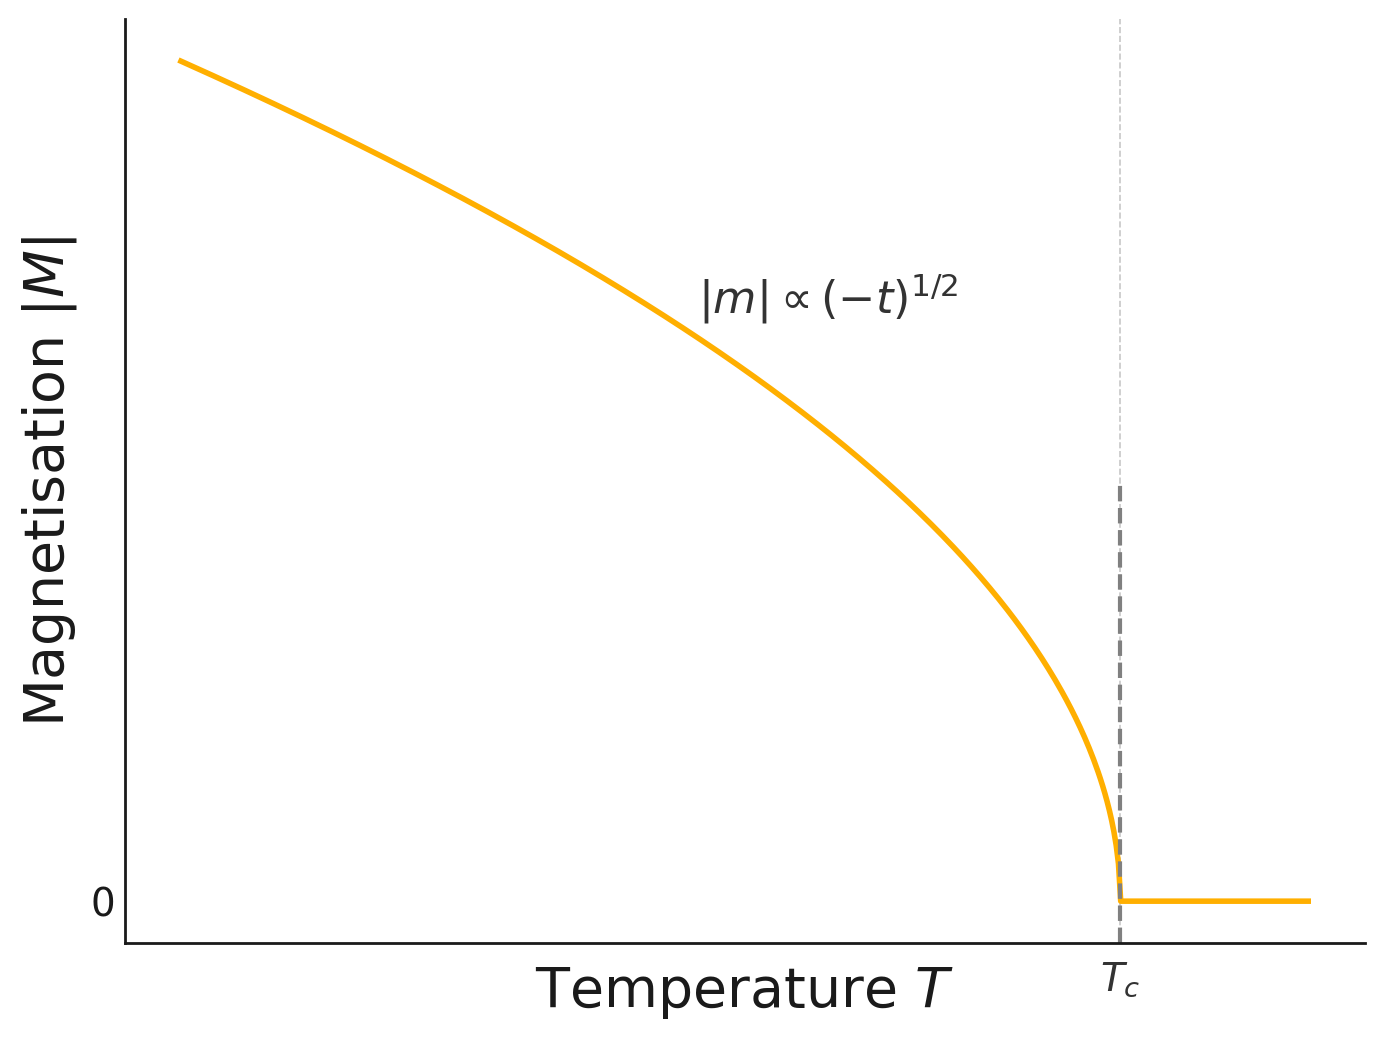
\includegraphics[width=1\linewidth,height=\textheight,keepaspectratio]{phase-transitions/Figs/mf_mag.png}

}

\subcaption{\label{fig-mfsum}Mean field behaviour of the Ising
magnetisation (schematic)}

\end{minipage}%
%
\begin{minipage}{0.50\linewidth}

\centering{

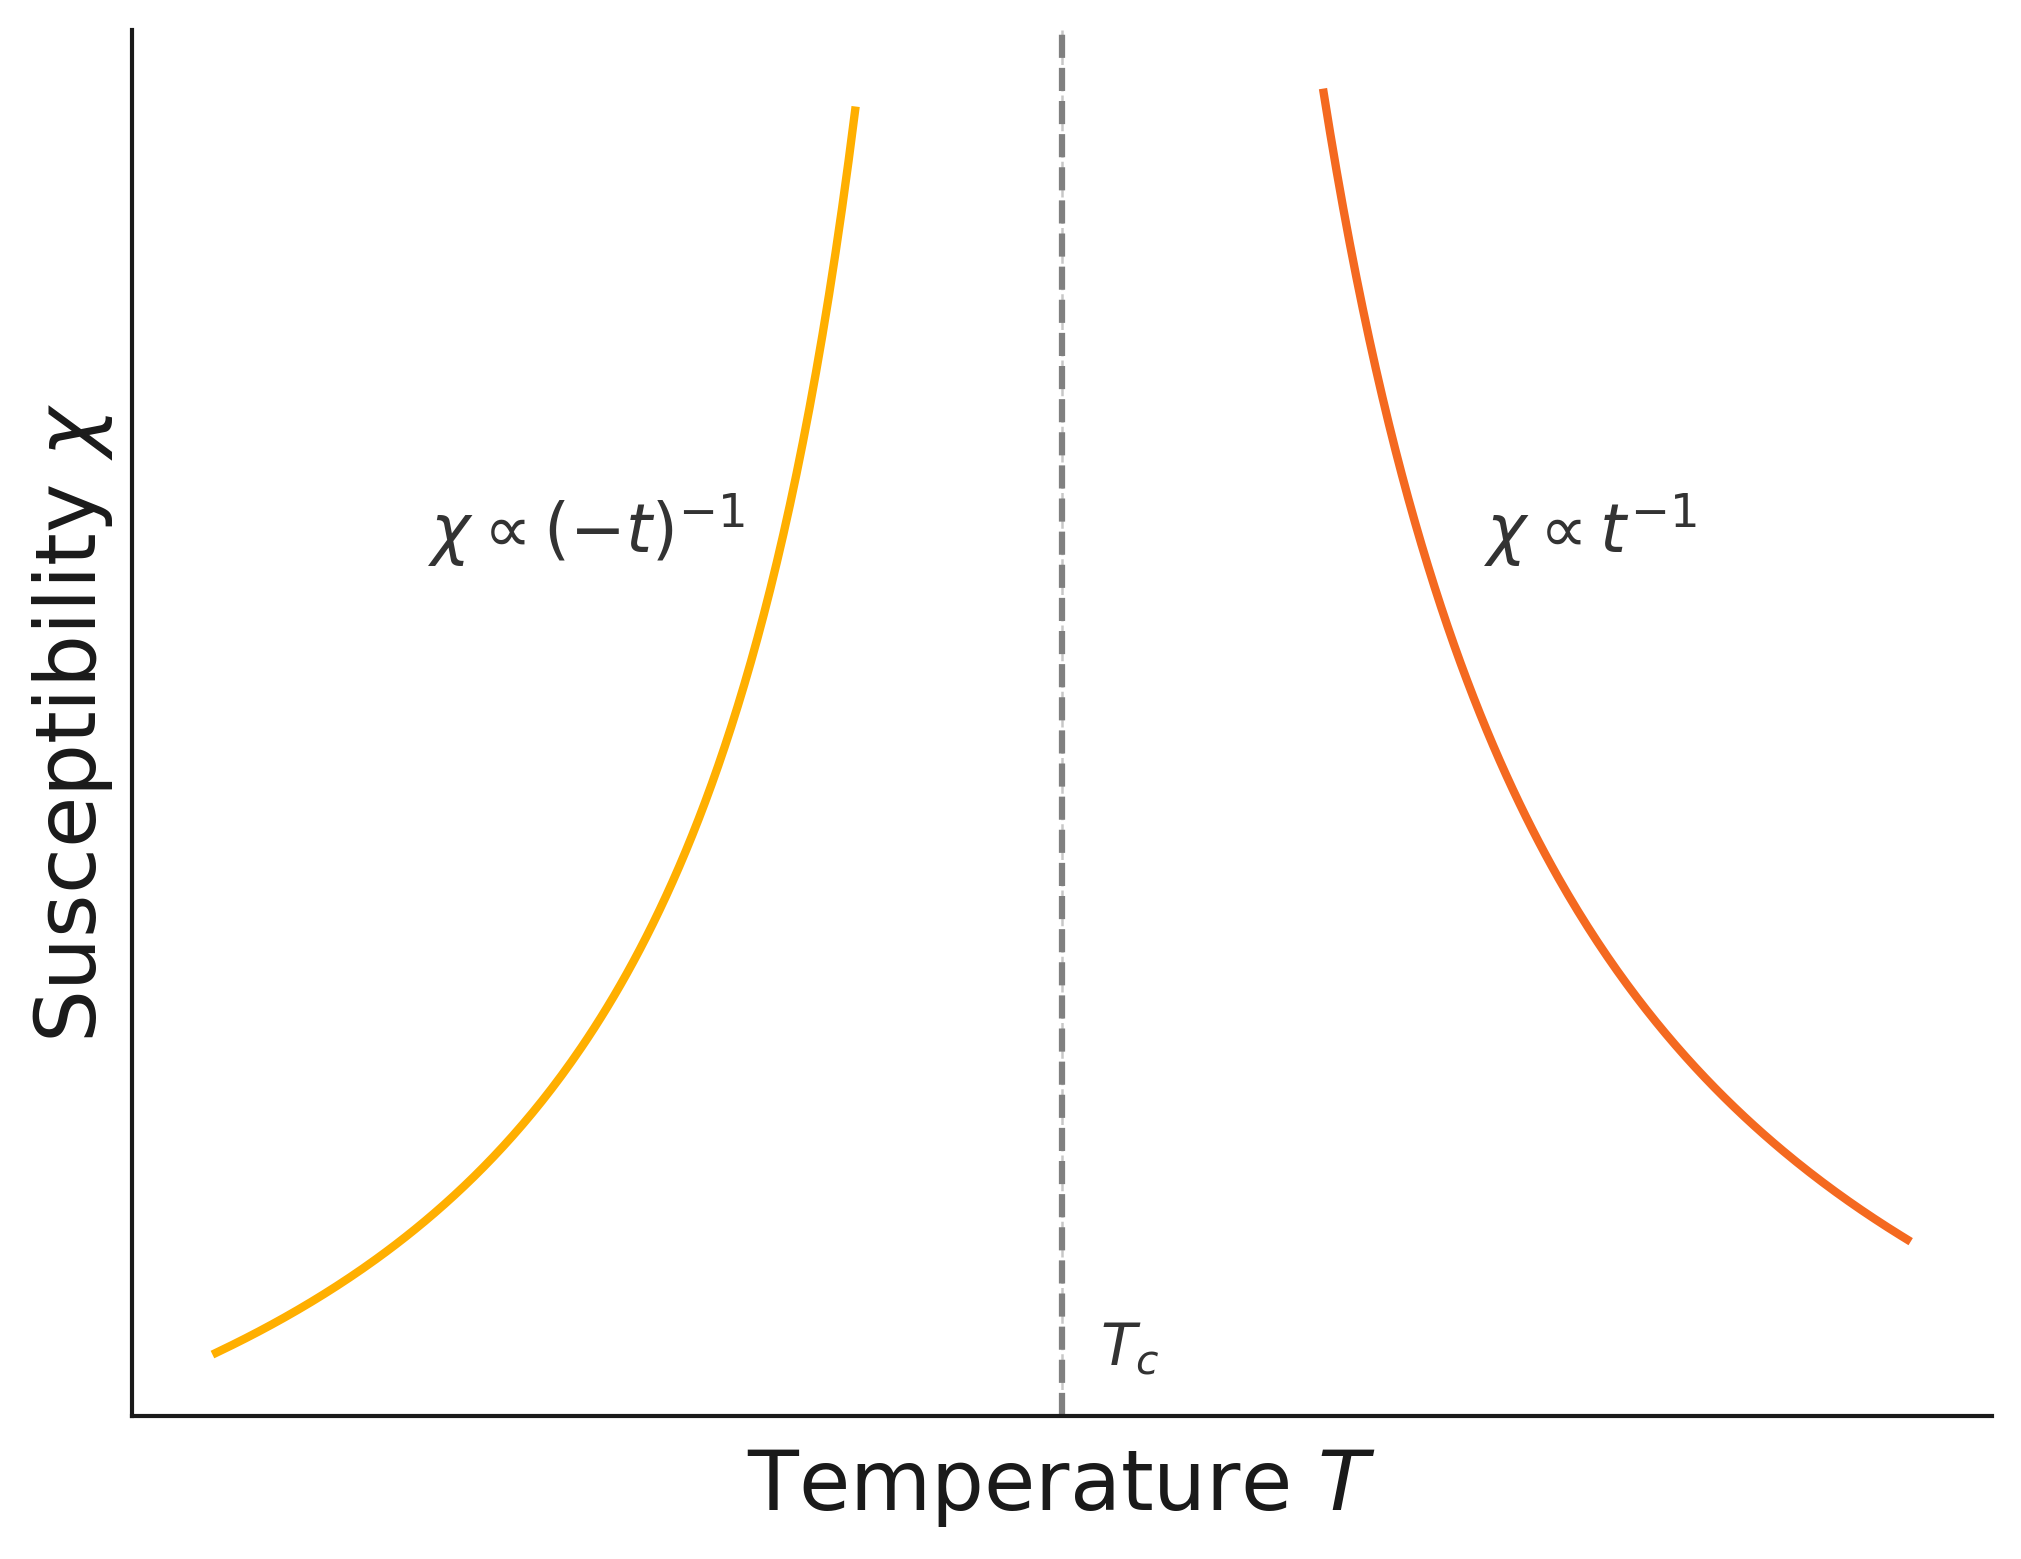
\includegraphics[width=1\linewidth,height=\textheight,keepaspectratio]{phase-transitions/Figs/mf_chi.png}

}

\subcaption{\label{fig-mfsum}Mean field behaviour of the Ising
susceptibility (schematic)}

\end{minipage}%

\end{figure}%

\section{Landau theory}\label{sec-landau-theory}

Landau theory is a slightly more general type of mean field theory than
that discussed in the previous subsection because it is not based on a
particular microscopic model. Its starting point is the Helmholtz free
energy, which Landau asserted can be written in terms of power series
expansion of the order parameter \(\phi\):

\[
F_(\phi)=\sum_{i=0}^{\infty}a_i\phi^i
\] The equilibrium value of \(\rho\) is that which minimises the Landau
free energy.

\begin{tcolorbox}[enhanced jigsaw, leftrule=.75mm, bottomrule=.15mm, toprule=.15mm, colbacktitle=quarto-callout-caution-color!10!white, title=\textcolor{quarto-callout-caution-color}{\faFire}\hspace{0.5em}{A note on order parameters}, breakable, titlerule=0mm, opacitybacktitle=0.6, colback=white, coltitle=black, colframe=quarto-callout-caution-color-frame, bottomtitle=1mm, rightrule=.15mm, toptitle=1mm, left=2mm, opacityback=0, arc=.35mm]

We have already seen examples of these in earlier sections, e.g., for
the liquid-gas transition this was \[
\rho_{liq} - \rho_{gas}: \quad \textrm{difference in density of two coexisting phases},
\] while for the Ising magnet it is the magnetisation \(m\). Both
quantities vanish at the critical point. These are examples of
\emph{scalar} order parameters -- a single number is required to
represent the degree of order (\(n = 1\)).

In the absence of a symmetry-breaking field, the Landau free-energy
density \(f_L\) must have symmetry \(f_L(-\phi) = f_L(\phi)\) (Ising
case).

For some other systems, \(n\) component vectors are required in order to
represent the order:

\[
\boldsymbol{\phi} = (\phi_1, \phi_2, \dots, \phi_n)
\]

Then \(f_L(\boldsymbol{\phi})\) should be symmetric under \(O(n)\)
rotations in \(n\)-component \(\phi\)-space.

The table below lists examples of order parameters for various physical
systems.

\begin{longtable}[]{@{}
  >{\raggedright\arraybackslash}p{(\linewidth - 4\tabcolsep) * \real{0.3478}}
  >{\raggedright\arraybackslash}p{(\linewidth - 4\tabcolsep) * \real{0.5130}}
  >{\raggedright\arraybackslash}p{(\linewidth - 4\tabcolsep) * \real{0.1391}}@{}}
\toprule\noalign{}
\begin{minipage}[b]{\linewidth}\raggedright
Physical System
\end{minipage} & \begin{minipage}[b]{\linewidth}\raggedright
Order Parameter \(\varphi\)
\end{minipage} & \begin{minipage}[b]{\linewidth}\raggedright
Symmetry Group
\end{minipage} \\
\midrule\noalign{}
\endhead
\bottomrule\noalign{}
\endlastfoot
Uniaxial (Ising) ferromagnet & Magnetisation per spin, \(m\) &
\(O(1)\) \\
Fluid (liquid-gas) & Density difference, \(\rho - \rho_c\) & \(O(1)\) \\
Liquid mixtures & Concentration difference, \(c - c_c\) & \(O(1)\) \\
Binary (AB) alloy (e.g., \(\beta\)-brass) & Concentration of one of the
species, \(c\) & \(O(1)\) \\
Isotropic (vector) ferromagnet & \(n\)-component magnetisation,
\(\mathbf{m} = (m_1, m_2, \dots, m_n)\) & \(O(n)\) \\
& \(n = 2\): \emph{xy} model & \(O(2)\) \\
& \(n = 3\): Heisenberg model & \(O(3)\) \\
Superfluid He\(^4\) & Macroscopic condensate wavefunction, \(\Psi\) &
\(O(2)\) \\
Superconductor (\emph{s}-wave) & Macroscopic condensate wavefunction,
\(\Psi\) & \(O(2)\) \\
Nematic liquid crystal & Orientational order,
\(\langle P_2(\cos \theta)\rangle\) & \\
Smectic A liquid crystal & 1-dimensional periodic density & \\
Crystal & 3-dimensional periodic density & \\
\end{longtable}

\textbf{Notes:}

\begin{itemize}
\item
  In \textbf{superfluid} \(^4He\) the order parameter is \[
  \Psi = |\Psi| e^{i\theta},
  \] the \emph{complex wavefunction} of the macroscopic condensate. Both
  the amplitude \(|\Psi|\) and phase \(\theta\) must be specified, so
  this corresponds to \(n = 2\).\\
  \textbf{Superconductors} also correspond to \(n = 2\).
\item
  In a \textbf{nematic} liquid crystal, the \emph{orientational} order
  parameter is \[
  \langle P_2(\cos \theta) \rangle \equiv \frac{1}{2}\langle 3\cos^2 \theta - 1\rangle,
  \] where \(\theta\) is the angle a molecule makes with the average
  direction of the long axes of the molecules (known as the
  \emph{director} \(\hat{n}\)). Rotational symmetry is broken. For the
  case of an \(n\) component vector, the free energy should be a
  function of: \[
  \phi^2 \equiv |\boldsymbol{\phi}|^2 = \phi_1^2 + \phi_2^2 + \dots + \phi_n^2 = \sum_{i=1}^n \phi_i^2
  \] in the absence of a symmetry breaking field. Rotational symmetry is
  incorporated into the theory.
\end{itemize}

\begin{figure}[H]

\begin{minipage}{0.50\linewidth}

\centering{

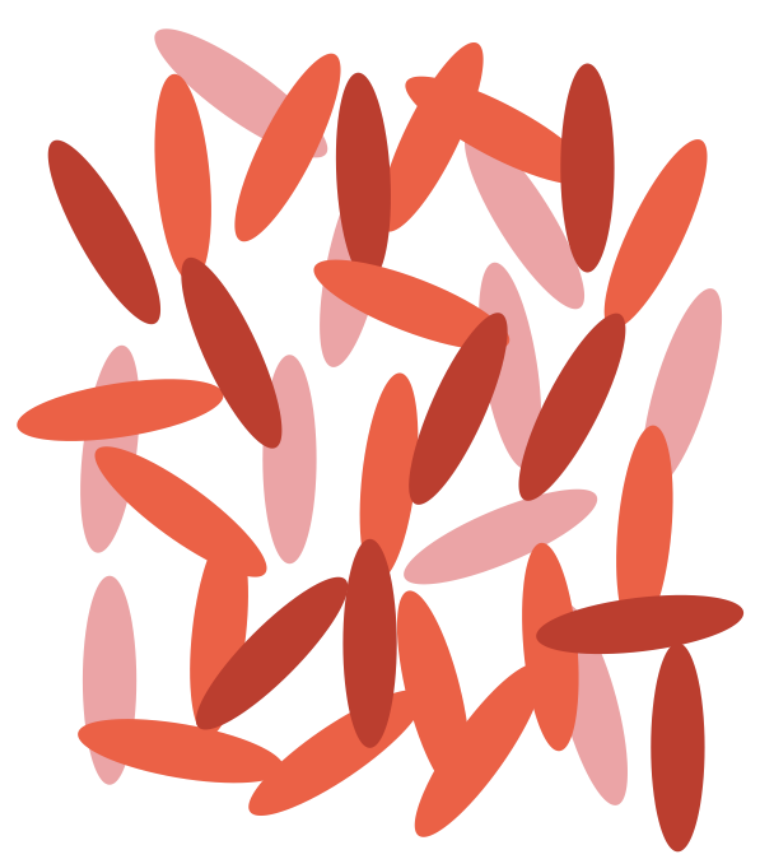
\includegraphics[width=0.5\linewidth,height=\textheight,keepaspectratio]{phase-transitions/Figs/isotropic-LC.png}

}

\subcaption{\label{fig-isotropic}Schematic of the isotropic liquid phase
of a system of elongated molcules.}

\end{minipage}%
%
\begin{minipage}{0.50\linewidth}

\centering{

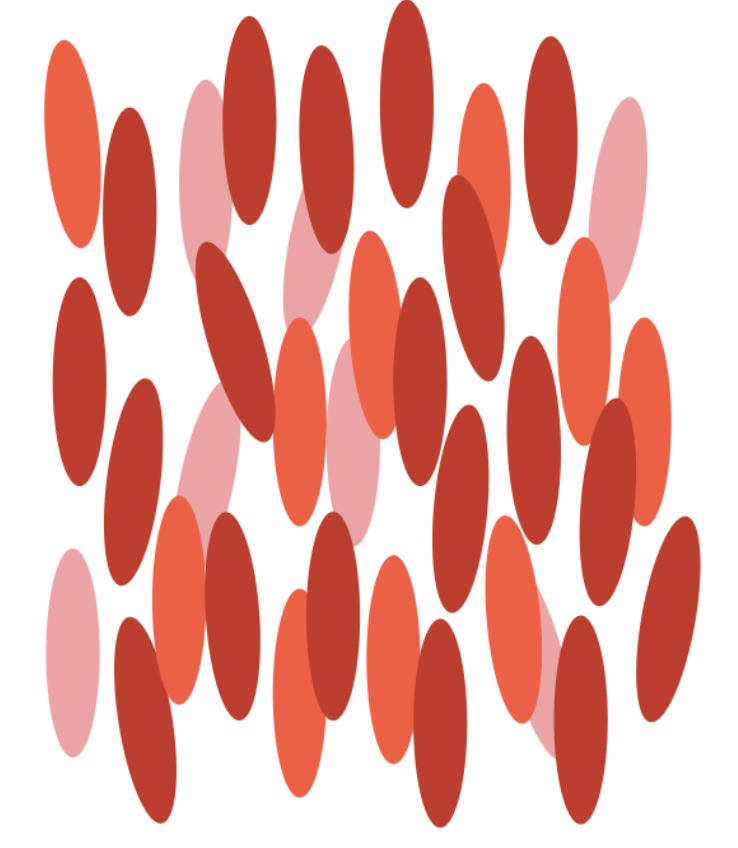
\includegraphics[width=0.5\linewidth,height=\textheight,keepaspectratio]{phase-transitions/Figs/nematic-LC.png}

}

\subcaption{\label{fig-isotropic}Schematic of the nematic liquid phase
of a system elongated molcules. This phase has uniaxial ordering.}

\end{minipage}%

\caption{\label{fig-mfsum}Isotropic and uniaxially ordered (nematic)
phases of liquid crystal molecules.}

\end{figure}%

\end{tcolorbox}

To exemplify the approach, let us specialise to the case of a
ferromagnet where \(\phi=m\), the magnetisation and write the Landau
free energy as

\begin{equation}\phantomsection\label{eq-landau}{
F(m)=F_0+a_2m^2+a_4m^4
}\end{equation}

Here only the terms compatible with the order parameter symmetry are
included in the expansion and we truncat the series at the 4th power
because this is all that is necessary to yield the essential
phenomenology. On symmetry grounds, the free energy of a ferromagnet
should be invariant under a reversal of the sign of the magnetisation.
Terms linear and cubic in \(m\) are not invariant under \(m\to -m\), and
so do not feature.

One can understand how the Landau free energy can give rise to a
critical point and coexistence values of the magnetisation, by plotting
\(F(m)\) for various values of \(a_2\) with \(a_4\) assumed positive
(which ensures that the magnetisation remains bounded). This is shown in
the following movie:

\url{Movies/landau_free_energy_evolution.mp4}

The situation is qualitatively similar to that discussed in
Section~\ref{sec-breaking}. Thermodynamics tells us that the system
adopts the state of lowest free energy. From the movie, we see that for
\(a_2>0\), the system will have \(m=0\), i.e.~will be in the disordered
(or paramagnetic) phase. For \(a_2<0\), the minimum in the free energy
occurs at a finite value of \(m\), indicating that the ordered
(ferromagnetic) phase is the stable one. In fact, the physical (up-down)
spin symmetry built into \(F\) indicates that there are two equivalent
stable states at \(m=\pm m^\star\). \(a_2=0\) corresponds to the
critical point which marks the border between the ordered and disordered
phases. Note that it is an inflexion point, so has
\(\frac{d^2F}{dm^2}=0\).

Clearly \(a_2\) controls the deviation from the critical temperature,
and accordingly we may write

\[a_2=\tilde{a_2} t\] where \(t\) is the reduced temperature. Thus we
see that the trajectory of the minima as a function of \(a_2<0\) in the
above movie effective traces out the coexistence curve in the \(m-T\)
plane.

We can now attempt to calculate critical exponents. Restricting
ourselves first to the magnetisation exponent \(\beta\) defined by
\(m=t^\beta\), we first find the equilibrium magnetisation,
corresponding to the minimum of the Landau free energy:

\begin{equation}\phantomsection\label{eq-minimize}{
\frac{dF}{dm}=2\tilde{a_2} tm+4a_4m^3=0
}\end{equation}

which implies

\[m\propto (-t)^{1/2},\] so \(\beta=1/2\), which is again a mean field
result.

Likewise we can calculate the effect of a small field \(H\) if we sit at
the critical temperature \(T_c\). Since \(a_2=0\), we have

\[F(m)=F_0+a_4m^4-Hm\]

\[\frac{\partial F}{\partial m}=0 \Rightarrow m(H,T_c)=\left(\frac{H}{4a_4}\right)^{1/3}\]

or

\[H \sim m^\delta ~~~~~ \delta=3\] which defines a second critical
exponent.

Note that at the critical point, a small applied field causes a very big
increase in magnetisation; formally, \((\partial m/\partial H)_T\) is
infinite at \(T=T_c\).

A third critical exponent can be defined from the magnetic
susceptibility at zero field

\[\chi=\left(\frac{\partial m}{\partial H}\right)_{T,V} \sim |T-T_c|^{-\gamma}\]

\emph{Exercise}: Show that the Landau expansion predicts \(\gamma=1\).

Finally we define a fourth critical exponent via the variation of the
heat capacity (per site or per unit volume) \(C_H\), in fixed external
field \(H=0\):

\[C_H \sim |T-T_c|^{-\alpha}\]

By convention, \(\alpha\) is defined to be positive for systems where
there is a \emph{divergence} of the heat capacity at the critical point
(very often the case). The heat capacity can be calculated from

\[C_H =-T\frac{\partial^2 F}{\partial T^2}\]

From the minimization over \(m\) @\#eq-minimize one finds
(\emph{exercise}: check this)

\begin{aligned}
F = & 0 ~~~~T>T_c\nonumber\\
F = & -a_2^2/4a_4 ~~~~ T < T_c
\end{aligned}

Using the fact that \(a_2\) varies linearly with \(T\), we have

\begin{aligned}
C_H =& 0 ~~~~ T\to T_c^+\nonumber\\
C_H =& \frac{T\tilde a_2^2}{2a_4} ~~~~ T \to T_c^-\:,
\end{aligned}

which is actually a step discontinuity in specific heat. Since for
positive \(\alpha\) the heat capacity is divergent, and for negative
\(\alpha\) it is continuous, this behaviour formally corresponds to
\(\alpha=0\)

\section{Shortcomings of mean field
theory}\label{shortcomings-of-mean-field-theory}

While mean field theories provide a useful route to understanding
qualitatively the phenomenology of phase transitions, in real
ferromagnets, as well as in more sophisticated theories, the critical
exponents are not the simple fraction and integers found here. This
failure of mean field theory to predict the correct exponents is of
course traceable to their neglect of correlations. In later sections we
shall start to take the first steps to including the effects of long
range correlations.

\phantomsection\label{tab-exponents}
\begin{longtable}[]{@{}ccccc@{}}
\caption{Comparison of true Ising critical exponents with their mean
field theory predictions in a number of dimensions.}\tabularnewline
\toprule\noalign{}
\endfirsthead
\endhead
\bottomrule\noalign{}
\endlastfoot
\(\:\) & Mean Field & \(d=1\) & \(d=2\) & \(d=3\) \\
Critical temperature \(k_BT/qJ\) & \(1\) & \(0\) & \(0.5673\) &
\(0.754\) \\
Order parameter exponent \(\beta\) & \(\frac{1}{2}\) & - &
\(\frac{1}{8}\) & \(0.325 \pm 0.001\) \\
Susceptibility exponent \(\gamma\) & \(1\) & \(\infty\) &
\(\frac{7}{4}\) & \(1.24 \pm 0.001\) \\
Correlation length exponent \(\nu\) & \(\frac{1}{2}\) & \(\infty\) &
\(1\) & \(0.63\pm 0.001\) \\
\end{longtable}

\part{Complex disordered systems}

\chapter{Entropy matters}\label{entropy-matters}

Most of the matter around us does not simply fit within the idealised
pictures of crystalline solids or simple liquids: examples include
colloids, polymers, surfactants, liquid crystals, foams, gels, and
biological materials such as proteins, DNA, and cell membranes.

This means that cellular \textbf{life itself} (the very constituents
that make us) obeys to principles that go beyond the standard patters of
conventional solid-state physics.

This branch of physics is called \textbf{soft condensed matter physics},
or \textbf{macromolecular} physics, or the physics of \textbf{complex
fluids}. Specifically, \emph{sof matter} refers to an area of condensed
matter focused on systems that can be \emph{easily deformed}.

In this course, we will emphasize the fact that many such systems are
not crystalline: thermal noise and disordered configurations play a key
role in their phase behavior, and hence we think of them as
\textbf{complex disordered systems}.

While we often think about problems in physics as a matter of energy
minimisation, in soft-matter physics a key role is played by the
\textbf{fluctuations}. Typically (but not exclusively) these are
\textbf{thermal fluctuations}. This means that \textbf{entropy} and not
only the energy from the interactions plays a key role.

\marginnote{\begin{footnotesize}

\end{footnotesize}}

This is because soft matter systems are typically composed of
\textbf{many microscopic constituents} in contact with an
\textbf{environment}. The appropriate description of the
\textbf{macroscopic state} of such systems is therefore
\textbf{statistical} and uses the language of \textbf{statistical
mechanics}. The relevant \textbf{energy}, therefore, is the free energy
of the statistical ensemble representative of the system under
consideration. For example, in the canonical ensemble, this is the
Helmholtz free energy

\[F = U-TS\]

where \(U\) is the internal energy, \(T\) the temperature and \(S\) is
the entropy of the system. Therefore, in a broader sense, soft matter is
the physics of those systems for which the internal energy and the
entropy are on comparable scales.

In other words, \textbf{fluctuations of the internal energy} are on the
same scale as \textbf{thermal fluctuations}:

\[\Delta U \sim k_BT \]

where \(k_B\) is the Bolztmann constant and \(\Delta U\) indicates
standard deviations from the average internal energy.

\begin{tcolorbox}[enhanced jigsaw, leftrule=.75mm, bottomrule=.15mm, toprule=.15mm, colbacktitle=quarto-callout-note-color!10!white, title=\textcolor{quarto-callout-note-color}{\faInfo}\hspace{0.5em}{The Physics of Entropy}, breakable, titlerule=0mm, opacitybacktitle=0.6, colback=white, coltitle=black, colframe=quarto-callout-note-color-frame, bottomtitle=1mm, rightrule=.15mm, toptitle=1mm, left=2mm, opacityback=0, arc=.35mm]

Soft matter physics is fundamentally the physics of \textbf{entropy}.
Unlike traditional systems where interaction energy minimization
dominates, in soft matter, entropy plays a crucial role in determining
the structure, dynamics, and behaviour of the system. The interplay
between entropy and intermolecular energy leads to the rich and diverse
phenomena observed in soft matter systems.

\end{tcolorbox}

\section{Systems and definitions}\label{systems-and-definitions}

\subsection{Elementary constituents and energy
scales}\label{elementary-constituents-and-energy-scales}

Soft matter covers a wide spectrum of deformable systems. Each is
constituted of many parts . Each is deformable because the interactions
amongst such parts are \textbf{weak} compared to the perturbing forces
(e.g.~thermal fluctuations or mechanical loading).

In hard condensed matter, the elementary constituents are the atoms
themselves, eventually with their subatomic particles. Between atoms,
the scale of the interaction energies is in the 0.1 to 10 eV: for
example the carbon-carbon covalent bond is approximately 3.6 eV.

The main units of soft matter are not atoms. They are instead themselves
aggregates of atoms such as:

\begin{itemize}
\tightlist
\item
  \textbf{colloids}, micrometer- to nanometer-sized particles dispersed
  in a fluid.
\item
  \textbf{polymers}, macromolecules composed of long chains such as DNA,
  proteins, plastics
\item
  \textbf{surfactants}, macromolecules wuth polar head and tails that
  lead to the spontaneous formation of structures such as bilayers
  (e.g.~the cellular membrane).
\end{itemize}

Amongst such units, the dominating forces of soft matter are much weaker
than in hard condensed matter:

\begin{itemize}
\tightlist
\item
  Van der Waals forces are of the order of 0.001-0.01 eV
\item
  weak interactions such as hydrogen-bonds are typically in the 0.01-0.2
  eV range
\item
  the thermal energy at room temperature is \(k_B T \approx 0.025 eV\)
  (check it for yourself)
\end{itemize}

At the \textbf{microscopic} level, all these interactions have
essentialy one source: the electrostatic force. However, this
information is practically of no use when we want to understand how the
units of soft matter come together to give rise to \textbf{macroscopic}
properties of soft matter systems, such as their elastic properties,
their viscosities, their plasticity. In fact, the emphasis on the
atomistic details of the various units is fundamentally misleading:
atomistically very different objects (e.g.~colloids and micelles) can in
fact share very similar macroscopic behaviours.

Therefore, theories of soft matter leverage the concept of
\textbf{coarse-graining}, rooted in the renormalisation group notions
explored earlier. Coarse-graining means integrating out the unimportant
degrees of freedom and only describing the units in terms of a few
important parameters. For example, instead of taking a full atomistic
representation of the DNA we may want to focus on the fact that
structurally it is a long chain with specific bending energies: we may
want to include the fact that it is formed by a double helix but we may
not want to specifically construct every single atom in the sugar chain
the forms the backbone. An example of DNA coarse garining is provided by
the succesful model
\href{https://dna.physics.ox.ac.uk/index.php/Main_Page}{oxDNA} (see
picture below):

\begin{figure}[H]

{\centering \pandocbounded{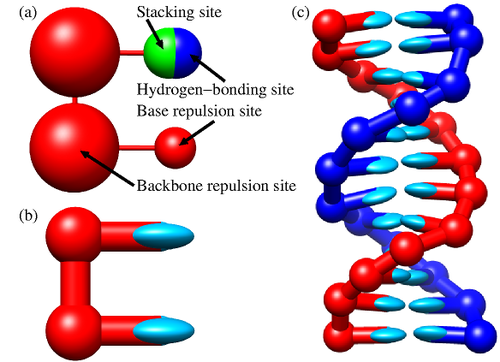
\includegraphics[keepaspectratio]{soft-matter/figs/The_model_half.png}}

}

\caption{oxDNA model: (a) Base structure on one strand; (b) planarity of
the bonding; (c) an example of the resulting double strand.}

\end{figure}%

\begin{tcolorbox}[enhanced jigsaw, leftrule=.75mm, bottomrule=.15mm, toprule=.15mm, colbacktitle=quarto-callout-note-color!10!white, title=\textcolor{quarto-callout-note-color}{\faInfo}\hspace{0.5em}{Coarse graining}, breakable, titlerule=0mm, opacitybacktitle=0.6, colback=white, coltitle=black, colframe=quarto-callout-note-color-frame, bottomtitle=1mm, rightrule=.15mm, toptitle=1mm, left=2mm, opacityback=0, arc=.35mm]

Coarse graining is often motivated by intuition, experimental insights
or a simple desire of simplification. It allows for a multi-scale
description of the problem which permits to describe large systems and
log time scales.

Nonetheless, coarse-graining can also be made mathematically rigorous.
For example, rigorous coarse graining in statistical mechanics can be
performed by projecting the dynamics onto a relevant and an irrelevant
(fluctutating) part, in the so called
\href{https://en.wikipedia.org/wiki/Mori-Zwanzig_formalism}{\textbf{Mori-Zwanzig}
formalism} {[}@mori1965{]}.

\end{tcolorbox}

\subsection{Classes of systems}\label{classes-of-systems}

In our exploration of soft matter we will focus on six main classes of
systems which display different physics:

\begin{itemize}
\tightlist
\item
  colloidal dispersions
\item
  polymeric systems
\item
  liquid crystals
\item
  surfactant aggregates
\item
  arrested systems
\item
  active matter
\end{itemize}

\subsubsection*{Colloidal dispersions}\label{colloidal-dispersions}
\addcontentsline{toc}{subsubsection}{Colloidal dispersions}

Colloidal dispersions are systems where small particles, typically in
the nanometer to micrometer range, are dispersed in a continuous medium
(a solvent). Prototypical colloids are \textbf{spherical} particles of
various sizes (e.g.~as those present in paint) but colloidal science has
achieved a high degree of sophistication, with colloidal particles with
various different shapes and interactions.

Colloids are often thought as \textbf{big atoms}: they exhibit Brownian
motion, can form ordered structures (colloidal crystals), and display
phase transitions similar to atomic systems. However, their larger size
and slower dynamics make them ideal for studying phenomena that are
difficult to observe in atomic systems.

\subsubsection*{Polymeric systems}\label{polymeric-systems}
\addcontentsline{toc}{subsubsection}{Polymeric systems}

Polymer physics is a field on its own. Polymers are macromolecules
composed of repeating structural units (monomers) connected by covalent
bonds. Their unique properties arise from their string-like structure
and the interplay between entropic and energetic contributions.

Polymers can be classified into two main categories:

\begin{itemize}
\tightlist
\item
  \textbf{Synthetic polymers}, including plastics (e.g., polyethylene,
  polystyrene) and synthetic rubbers.
\item
  \textbf{Biopolymers}, such as polymers like DNA, RNA, and proteins.
\end{itemize}

Compared to colloids, polymers have distiunctive characteristics common
to all chain-like molecules, such as their topological constraints due
to teh fact that two polymers cannot cross each other (a phenomenon
known as \emph{polymer entanglement}).

\subsubsection*{Liquid crystals}\label{liquid-crystals}
\addcontentsline{toc}{subsubsection}{Liquid crystals}

When we take soft matter units that are highly anisotropic
(e.g.~elongate in particular directions) thermal fluctuations and high
packing lead to equilibrium states woth a degree of order that is
intermediate between the complete disorder of a liquid and the
long-ranged, three-dimensional order of a crystal.

Such states are referred to as \textbf{liquid crystal} and can be
described successffully with continuum free energy theories that take
into account the symmetries of the order parameters.

Components that form liquid crystals are called \textbf{mesogens} and
include highly anisotropic organic macromolecules (as used in liquid
crystal displays), rod-like molecules or polymeric aggregates, as well
as disk-shaped molecules and particles(such as triphenylene and
derivatives).

\subsubsection*{Surfactant aggregates}\label{surfactant-aggregates}
\addcontentsline{toc}{subsubsection}{Surfactant aggregates}

When two distinct fluid phases are put into contact, a free energy cost
per unit area ensues: this is the surface tension. It is possible to
control the tension by introducing molecules that sit at the interface
between the two phases, called \textbf{surfactants}.

Hence, surfactants are molecules which contain chemical groups with
different affinities (they are \textbf{amphiphilic}). A key example is
the case of phospholipids, which posses both hydrophilic
(water-preferring) heads and hyrdrophobic (water avoiding) tails. As
surfactants sit at inetrface they are able to \textbf{self-assemble} and
separate different fluid phases, forming equilibrium bilayers and
vesicles that are ubiquitous in cell biology.

\subsubsection*{Arrested systems}\label{arrested-systems}
\addcontentsline{toc}{subsubsection}{Arrested systems}

We have stressed that the thermal energy is distinctive of soft matter
systems. It would be then natural to assume that as we reduce the
temperature, we should converge readily to the solid state physics of
crystalline solids. In fact, on the way to low temperatures, the lack of
long-range order of most soft-matter systems has important consequences:
many such systems find themselves trapped in states that are not
corresponding to the global energy minimum (i.e.~the crystal) and
instead display non trivial mechanisms of structural relaxation. These
systems are disordered a bit like liquids, but share various mechanical
properties, such as emergence rigidity, elasticity and plasticity.

Examples of arrested systems include:

\begin{itemize}
\tightlist
\item
  \textbf{Glasses}, such as silica glass or metallic glasses, where the
  system is kinetically trapped in a disordered state.
\item
  \textbf{Gels}, which are networks of interconnected particles or
  polymers that span the entire system, providing rigidity despite being
  mostly liquid.
\end{itemize}

These systems are arrested as their relaxation towards equilibrium is so
slow that is longer than any observable timescales. This makes them
fundamentally \textbf{out-of-equilibrium} systems, escaping from an
ordinary description in terms of equilibrium statistical mechanics.

\subsubsection*{Active matter}\label{active-matter}
\addcontentsline{toc}{subsubsection}{Active matter}

Active matter refers to systems composed of units that consume energy to
generate motion or mechanical stresses. Unlike passive systems, active
matter is inherently out of equilibrium due to the continuous energy
input at the microscopic level. Examples include:

\begin{itemize}
\tightlist
\item
  \textbf{Biological systems}, such as bacterial colonies, cell tissues,
  and flocks of birds.
\item
  \textbf{Synthetic systems}, like self-propelled colloids or active
  gels.
\end{itemize}

The study of active matter focuses on understanding how individual
activity leads to emergent collective behaviors, such as swarming,
clustering, or pattern formation, often described using hydrodynamic
theories or agent-based models.

\chapter{Colloids}\label{colloids-1}

\begin{Shaded}
\begin{Highlighting}[]
\NormalTok{\#| echo: false}
\NormalTok{\#| autorun: true}
\NormalTok{\# modifying the path to add the code folder}
\NormalTok{import sys}
\NormalTok{sys.path.insert(0, \textquotesingle{}src\textquotesingle{})}
\end{Highlighting}
\end{Shaded}

\section{Kinds of colloids}\label{kinds-of-colloids}

Colloids are mixtures where one substance is dispersed throughout
another. They consist of particles that are larger than typical
molecules but small enough to remain suspended without settling.
Examples include milk, fog, and paint.

Colloids can be classified based on the state of the \textbf{dispersed
phase} and the \textbf{dispersion medium}. Depending on the particular
mixture, one can obtain a wide variety of soft materials, with unique
mechanical, optical, and thermal properties.

\begin{longtable}[]{@{}
  >{\raggedright\arraybackslash}p{(\linewidth - 4\tabcolsep) * \real{0.2184}}
  >{\raggedright\arraybackslash}p{(\linewidth - 4\tabcolsep) * \real{0.4023}}
  >{\raggedright\arraybackslash}p{(\linewidth - 4\tabcolsep) * \real{0.3678}}@{}}
\toprule\noalign{}
\begin{minipage}[b]{\linewidth}\raggedright
Dispersion Phase
\end{minipage} & \begin{minipage}[b]{\linewidth}\raggedright
\end{minipage} & \begin{minipage}[b]{\linewidth}\raggedright
Dispersion Medium
\end{minipage} \\
\midrule\noalign{}
\endhead
\bottomrule\noalign{}
\endlastfoot
& Solid & Liquid \\
Solid & \begin{minipage}[t]{\linewidth}\raggedright
\emph{Solid suspension:}\\
pigmented plastics,\\
stained glass,\\
ruby glass, opal, pearl\strut
\end{minipage} & \begin{minipage}[t]{\linewidth}\raggedright
\emph{Sol, colloidal suspension:}\\
metal sol,\\
toothpaste, paint,\\
ink, clay slurries, mud\strut
\end{minipage} \\
Liquid & \begin{minipage}[t]{\linewidth}\raggedright
\emph{Solid emulsion:}\\
bituminous road paving,\\
ice cream\strut
\end{minipage} & \begin{minipage}[t]{\linewidth}\raggedright
\emph{Emulsion:}\\
milk, mayonnaise,\\
butter, pharmaceutical creams\strut
\end{minipage} \\
Gas & \begin{minipage}[t]{\linewidth}\raggedright
\emph{Solid foam:}\\
zeolites, expanded polystyrene,\\
`silica gel'\strut
\end{minipage} & \begin{minipage}[t]{\linewidth}\raggedright
\emph{Foam:}\\
froths, soap foam,\\
fire-extinguisher foam\strut
\end{minipage} \\
\end{longtable}

Clearly, colloidal materials form an incredibly diverse class, and
surround us in our everyday lives. Here are some visual examples from
the table above:

\begin{figure}[H]

{\centering \pandocbounded{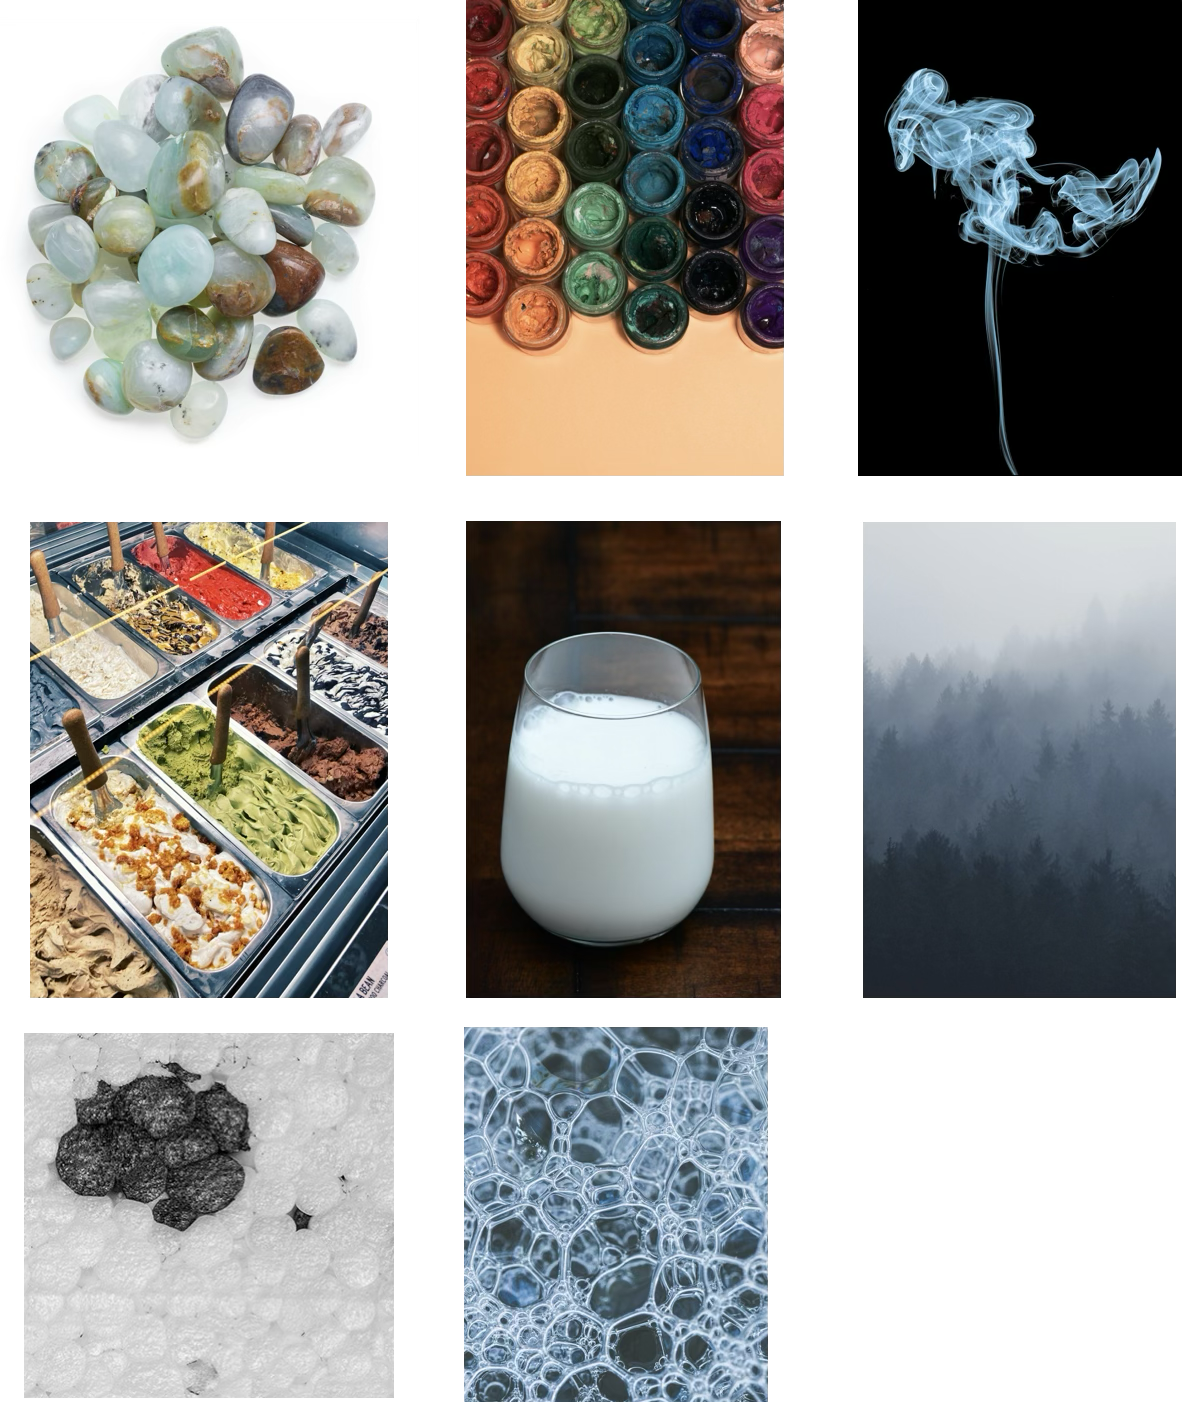
\includegraphics[keepaspectratio]{soft-matter/figs/colloids.png}}

}

\caption{First row: opal, paint, smoke. Middle row: ice-cream
(\emph{gelato}), milk, fog. Bottom row: expanded polystyrene and foam.
Source: unsplash.com}

\end{figure}%

The \href{https://goldbook.iupac.org/terms/view/C01172}{IUPAC definition
of colloids} is based on the idea that the particles are dispersed in a
medium, creating a \emph{subdivision} at the \textbf{colloidal scale}:
approximately 1nm to 1µm.

The small sizes of colloids means that they are constantly subject to
the collisions with the atom/molecules/particle of the medium, triggered
by thermal fluctuations. Due to this, the colloids undergo
\href{../phase-transitions/Brownian-and-Langevin-dynamics.qmd}{Brownian
motion}. For each particle, the amount of energy received from the
medium is of the order of \(k_B T\) (the reference energy scale of
thermal soft matter). This energy can be compared with the the potential
energy to produce a dimensionless number, the \textbf{gravitational
Péclet number}

\[{\rm Pe}_g = \dfrac{\Delta m g R}{k_B T}\]

where \(R\) is the radius of the colloid respectively, \(g\) is the
acceleration due to gravity, and \(\Delta m\) is the \emph{buoyant
mass}, which for a spherical colloid is expressed as
\(\Delta m = \dfrac{4\pi}{3}\Delta\rho R^3\), with \(\Delta \rho\) being
the density difference between the particle and the dispersion medium
(the \emph{solvent}). We have a colloidal suspension only when
\({\rm Pe}_g \lesssim 1\), i.e.~when Brownian motion is only marginally
perturbed by the effects of gravity.

\section{Stability of colloids and colloid-colloid
interactions}\label{stability-of-colloids-and-colloid-colloid-interactions}

A colloidal dispersion is said to be \textbf{stable} if it is able to
remain dispersed and Brownian for a long time (typically, significantly
longer than the experimental observation time). Unstable colloids
undergo aggregation or sedimentation due to the dominance of attractive
forces or gravity.

For example, consider a colloidal suspension like milk. Milk is an
emulsion where fat droplets are dispersed in water and stabilised by
proteins. If lemon juice (an acid) is added, the dispersion medium
(water) changes, the pH drops, and the emulsion is \emph{destabilised}.
This causes the proteins to coagulate, leading to the separation of
curds (solid) and whey (liquid).

\begin{figure}[H]

{\centering \pandocbounded{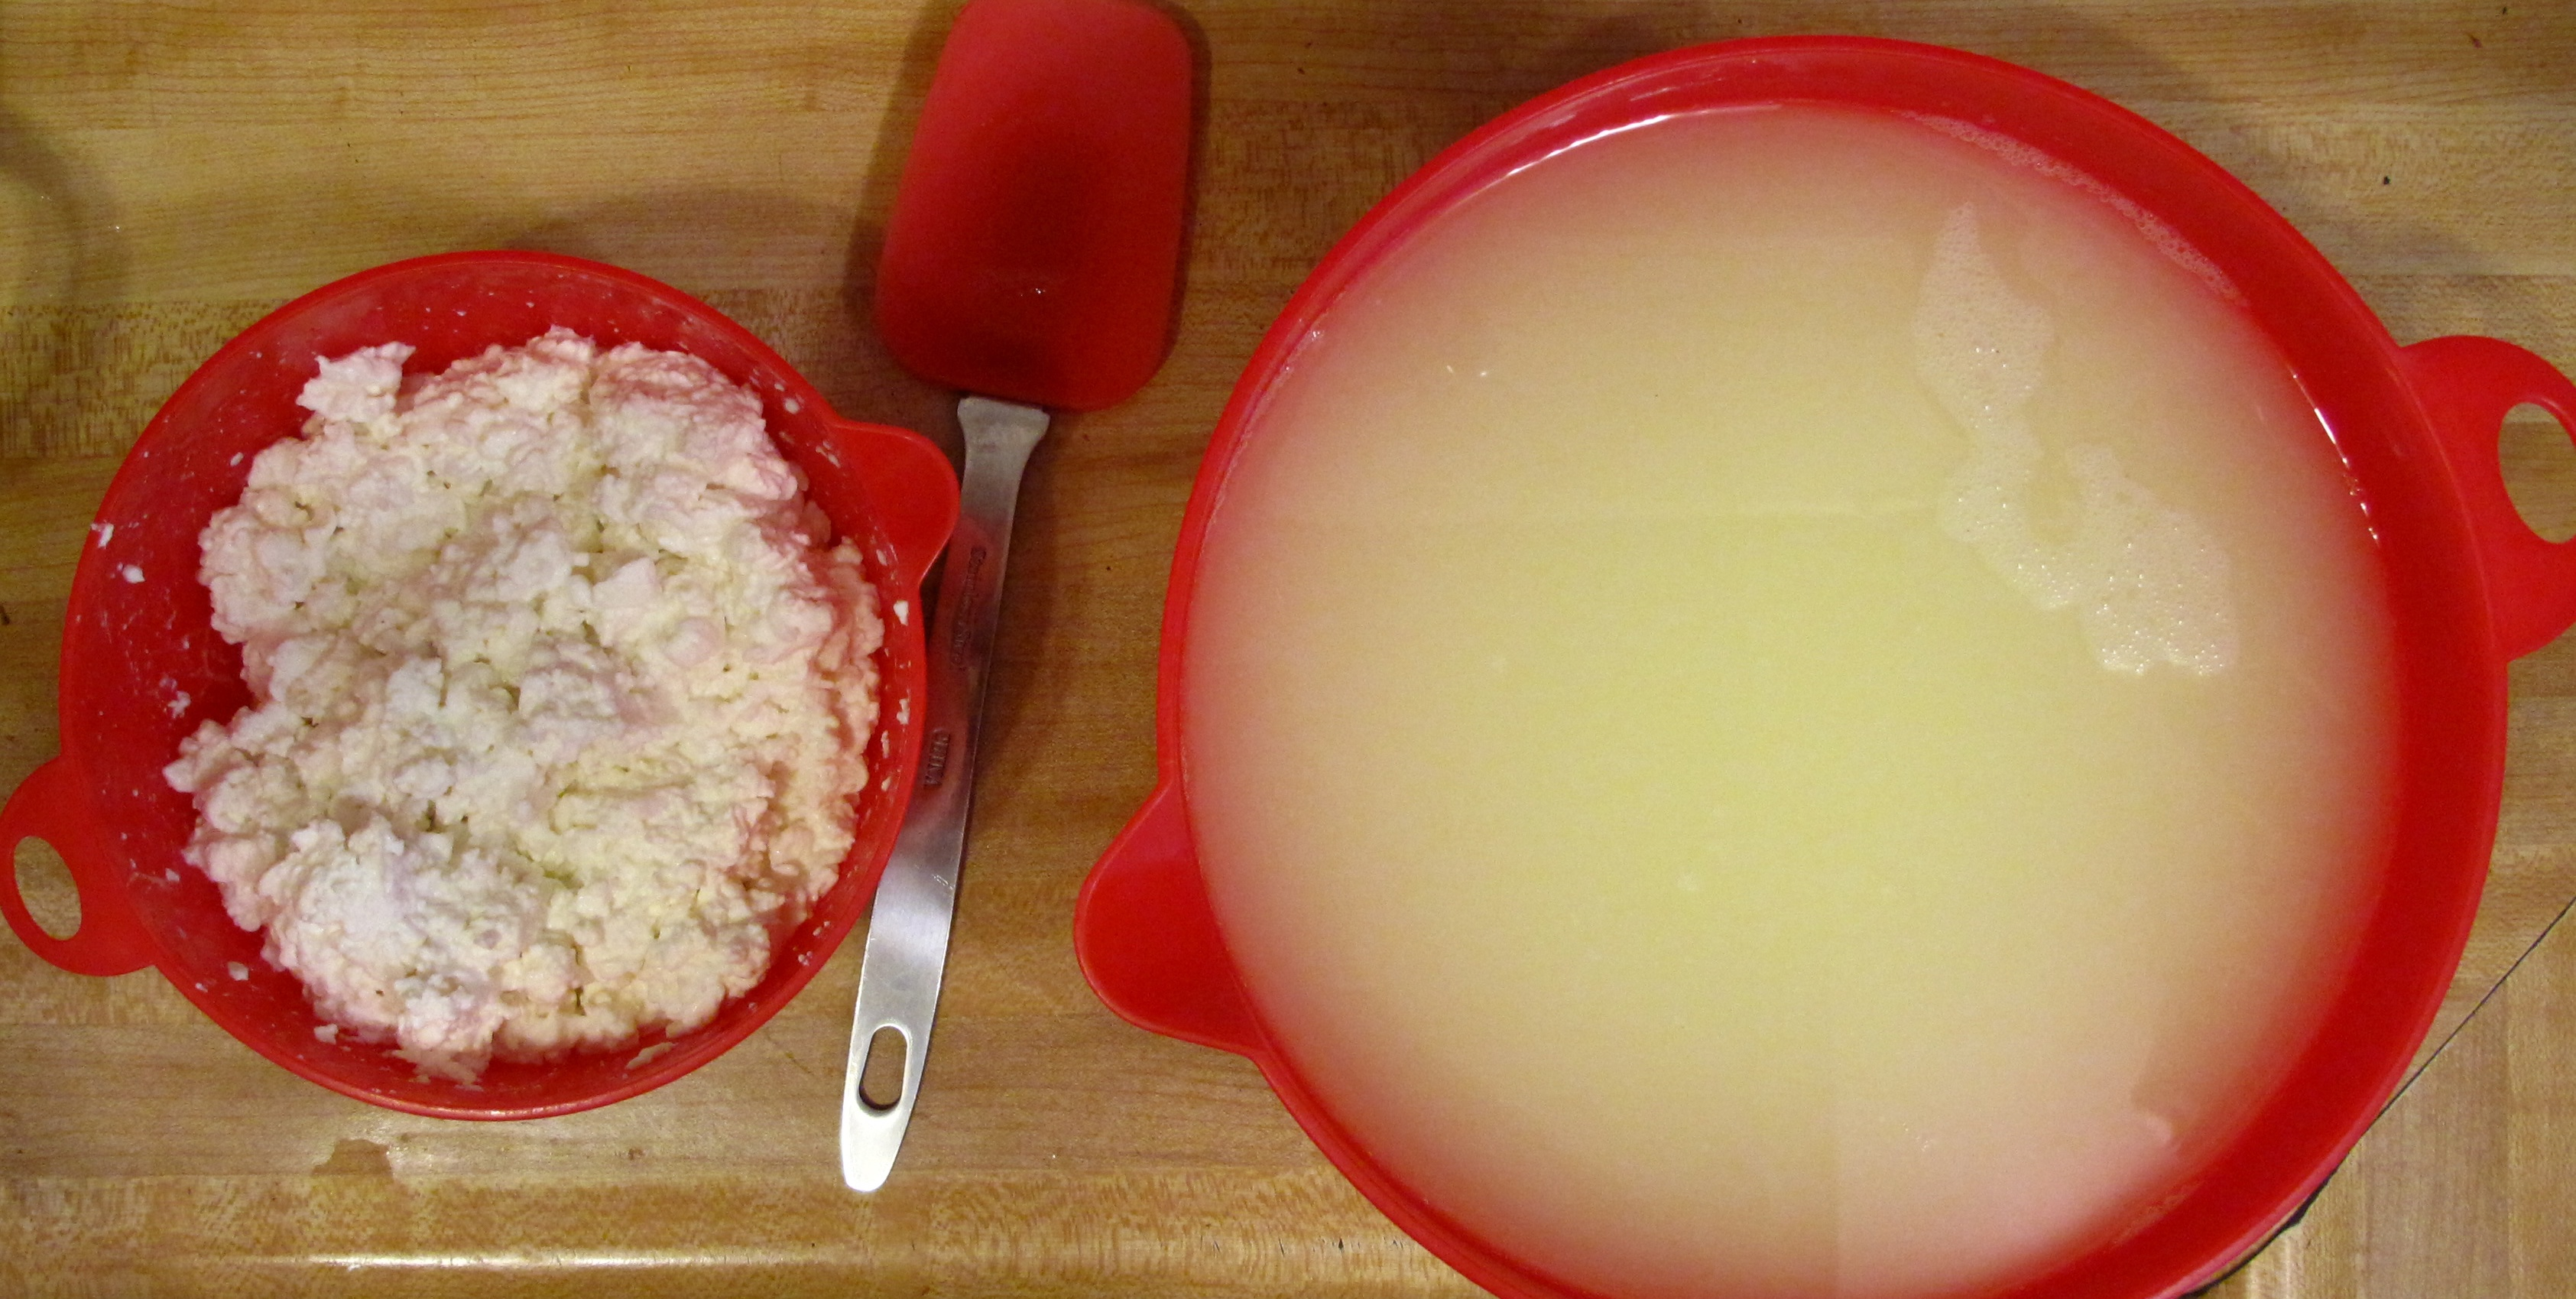
\includegraphics[keepaspectratio]{soft-matter/figs/Curds_and_whey.jpg}}

}

\caption{Curds and whey resulting from the destabilisation of milk, a
colloidal emulsion. (Wikimedia)}

\end{figure}%

It is clear from this example that the nature of the dispersed phase and
the dispersed medium ultimately determine the stability of colloidal
dispersions. What ultimately matters for the stability is whether the
colloids have a propensity to aggregate or not. This propensity is
quantified in terms of \textbf{colloidal interactions}.

\subsection{Fundamental and effective
forces}\label{fundamental-and-effective-forces}

At the colloidal scales, only two kinds of fundamental forces are
relevant: gravity and electro (and occasionally magneto) static forces.
As we have seen above, when a system is truly colloidal, gravitational
contributions are assumed to be small, so in effect for a non magnetic
colloid (which is the vast majority of colloidal systems) only
electrostatic forces are fundamentally important.

However, colloidal dispersions consist of large particles carrying many
charges both in the dispersed phase and the surrounding medium, arranged
disorderly at the atomic scale. This makes a microscopic description of
all charges and the resulting electrostatic fields not only unfeasible
but also ineffective for understanding colloidal systems in terms of key
characteristics such as particle size, density, and spatial
distribution. The fundamental issue is the one of time-scales: the
motion of colloids is much slower than the motion of individual ions or
molecules. Over such longer timescales, many interactions at the
\textbf{microscopic} atomistic scale take place and we can think of
taking averages to extract \textbf{macroscopic}, \textbf{effective}
interactions at the colloidal scale \footnote{This is clearly an
  instance of the idea of \textbf{coarse graining} that we have
  introduced \hyperref[entropy-matters]{earlier}.}.

This is especially important due to \textbf{quantum fluctuations}: the
uncertainty principle means that electron clouds around atoms are not
fixed but exhibit intrinsic fluctuations in their charge distribution.
Perturbative approaches allow us to capture the effective forces
resulting from such fluctuations.

There are many examples of such effective forces
{[}@lekkerkerker2024colloids{]}. One you may already know is the Van der
Waals interaction. For colloids, we have additional relevant forces,
such as the double layer interaction and the depletion interaction. We
detail them here below.

\subsection{Van der Waals interaction}\label{van-der-waals-interaction}

The London-van der Waals \textbf{dispersion forces} arise from the
interaction between \textbf{instantaneous dipoles} in overall neutral
atoms or molecules. We know from classical electrostatics that static
dipoles interact via the dipole-dipole interaction, with a potential
strength which decays like \(1/r^3\), where \(r\) is the separation
between two dipoles.

More in general, neutral atom or molecules have electronic clouds that
are fluctuating and not symmetrically distributed, creating a
\textbf{temporary dipole}. Such instantaneous dipole \textbf{induces} a
dipole in a neighboring atom or molecule by distorting its electron
cloud.

The interaction energy between two dipoles \(\mu_1\) and \(\mu_2\)
separated by a distance \(r\) is proportional to: \[
U \propto -\frac{\mu_1 \mu_2}{r^3}
\]

\marginnote{\begin{footnotesize}

\begin{figure}[H]

{\centering 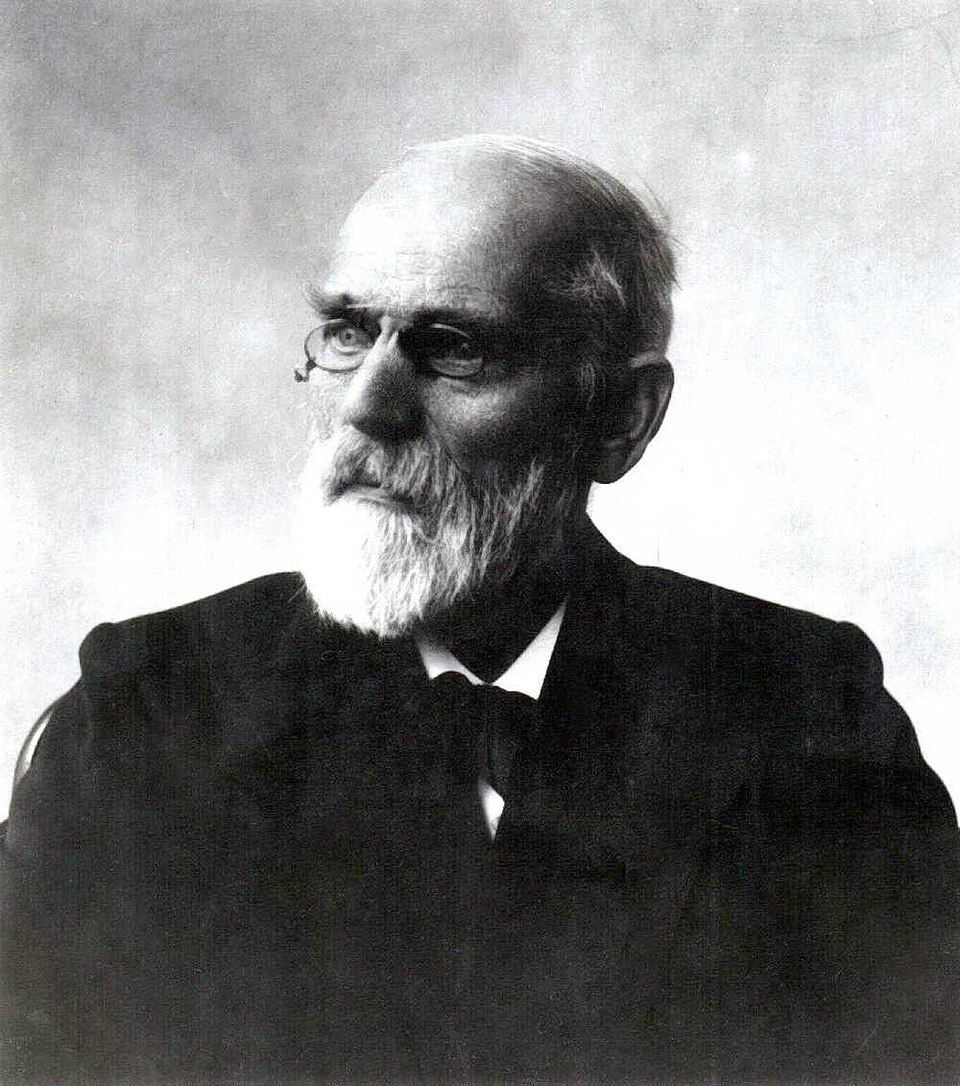
\includegraphics[width=1.5625in,height=\textheight,keepaspectratio]{soft-matter/figs/Johannes_Diderik_van_der_Waals.jpg}

}

\caption{Johannes Diderik van der Waals (1837-1923), who hypothesised
the existence of forces responsible for the non-ideal behaviour of
gases.}

\end{figure}%

\begin{figure}[H]

{\centering 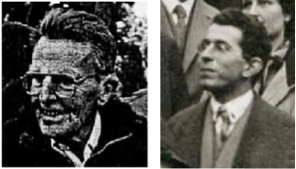
\includegraphics[width=3.125in,height=\textheight,keepaspectratio]{soft-matter/figs/hamaker-london.png}

}

\caption{Left: Hugo C. Hamaker (1905-1993), who explained the origin of
Van der Waals forces, and Fritz London (1900-1954), who quantified the
dispersion force.}

\end{figure}%

\end{footnotesize}}

The dipole moments fluctuate due to quantum mechanical effects. The
average interaction energy is derived using perturbation theory and is
proportional to the polarisabilities \(\alpha_1\) and \(\alpha_2\) of
the two particles:

\[
    U(r) = -\frac{C}{r^6}
\]

where \(C \propto \alpha_1 \alpha_2\) depends on the polarisabilities
and ionization energies of the particles.

The resulting \(r^{-6}\) dependence is also referred to as the
\textbf{London dispersion force}, which can be derived within
quantum-mechanical perturbation theory {[}@london1937general{]}.

We can then assume to take two identical spherical colloids of radius
\(R\) at distance \(h\) and that every volume element of such spheres
interacts with the London dispersion force (see the semi-classical
approach of Hamaker @hamaker1937london for illustration). Integrating
over all volume elements yields the collodial spheres \textbf{Van der
Waals attractive potential} in the form

\[W_{wdW}(h)=-\dfrac{A-H}{g}f(h/R)\]

where \(A_H\) is the \textbf{Hamaker constant} and \(f(h/R)\) is

\[f(h/R) = \left[ \frac{2R^2}{h^2 - 4R^2} + \frac{2R^2}{h^2} + \ln\left( \frac{h^2 - 4R^2}{h^2} \right) \right]\]

\begin{tcolorbox}[enhanced jigsaw, leftrule=.75mm, bottomrule=.15mm, toprule=.15mm, colbacktitle=quarto-callout-note-color!10!white, title=\textcolor{quarto-callout-note-color}{\faInfo}\hspace{0.5em}{Sketch of a derivation of colloid-colloid Van der Waals potential}, breakable, titlerule=0mm, opacitybacktitle=0.6, colback=white, coltitle=black, colframe=quarto-callout-note-color-frame, bottomtitle=1mm, rightrule=.15mm, toptitle=1mm, left=2mm, opacityback=0, arc=.35mm]

Each volume element in one sphere interacts with each in the other
sphere via:

\[
\phi(r) = -\frac{C}{r^6}
\]

So the total interaction energy is:

\[
U(h) = -C \iint \frac{1}{|\mathbf{r}_1 - \mathbf{r}_2|^6} \, dV_1 \, dV_2
\]

Let:

\begin{itemize}
\tightlist
\item
  Sphere 1 be centered at \((0, 0, 0)\),
\item
  Sphere 2 be centered at \((0, 0, h)\),
\item
  \(\mathbf{r}_1 = \mathbf{r}\), \(\mathbf{r}_2 = \mathbf{r}'\)
\end{itemize}

Then \(|\mathbf{r}_1 - \mathbf{r}_2| = |\mathbf{r} - \mathbf{r}'|\), and
the integral becomes:

\[
U(h) = -C \iiint_{|\mathbf{r}| \leq R} \iiint_{|\mathbf{r}' - h\hat{z}| \leq R} \frac{1}{|\mathbf{r} - \mathbf{r}'|^6} \, d^3\mathbf{r} \, d^3\mathbf{r}'
\]

Hamaker evaluated this by integrating over the \textbf{densities of
interacting atoms} with number density \(\rho\) in both spheres. The
result:

\[
U(h) = -\rho^2 C \iint \frac{1}{|\mathbf{r}_1 - \mathbf{r}_2|^6} \, dV_1 \, dV_2
\]

Defining the \textbf{Hamaker constant}:

\[
A_H = \pi^2 \rho^2 C
\]

So,

\[
U(h) = -\frac{A_H}{\pi^2} \iint \frac{1}{|\mathbf{r}_1 - \mathbf{r}_2|^6} \, dV_1 \, dV_2
\]

This six-dimensional integral can be evaluated analytically for spheres,
yielding:

\[
U(h) = -\frac{A_H}{6} \left[ \frac{2R^2}{h^2 - 4R^2} + \frac{2R^2}{h^2} + \ln\left( \frac{h^2 - 4R^2}{h^2} \right) \right]
\]

\end{tcolorbox}

\begin{Shaded}
\begin{Highlighting}[]
\NormalTok{\#| autorun: true}
\NormalTok{import numpy as np}
\NormalTok{import plotting}
\NormalTok{\# parameters: change them to explore the interaction!}
\NormalTok{R = 5.0  \# Radius of the colloid}
\NormalTok{A\_H = 1e{-}20  \# Hamaker constant (in Joules)}
\NormalTok{h = np.linspace(2.01 * R, 10+R*2, 1000)  \# Separation distance (h \textgreater{} 2R)}
\NormalTok{\# Van der Waals potential}
\NormalTok{def van\_der\_waals\_potential(h, R, A\_H):}
\NormalTok{    f\_h\_R = (2 * R**2 / (h**2 {-} 4 * R**2)) + (2 * R**2 / h**2) + np.log((h**2 {-} 4 * R**2) / h**2)}
\NormalTok{    return {-}A\_H * f\_h\_R}

\NormalTok{\# compute potential}
\NormalTok{W\_vdW = van\_der\_waals\_potential(h, R, A\_H)}
\NormalTok{\# convenience plotting function, you can use matplotlib if you prefer}
\NormalTok{plotting.simple\_plot(h,W\_vdW)}
\end{Highlighting}
\end{Shaded}

Van der Waals interactions are considered to be \textbf{short-range}
forces in the sense that their decay rate(e.g.~London's \(1/r^6\)) is
much faster than Coulombic interactions (\(1/r\)). Importantly, since
their origin resides in the fluctuation of charges on the colloids,
their strength is \emph{not additive}: simply summing all the pairwise
interactions does not fully accurately account for man-body effects. We
often rely on such two-body approximations, but we should be aware that
they are a simplified scenario.

\subsection{Double-layer interaction}\label{double-layer-interaction}

Colloids are often charged. The solution they are immersed also has an
\textbf{inhomogeneous} distribution of ions: there will be

\begin{itemize}
\item
  \textbf{co-ions} (same charge as the colloid) that will be pushed away
  from the colloid surface, while
\item
  \textbf{counter-ions} (opposite charge) will accumulate at the
  surface.
\end{itemize}

These two different concentrations of oppositely charged ions form what
is called a \textbf{double layer} and its property (such as its width)
are obviously controlled by the number of ions in the solvent, which can
be tuned by adding or removing, for example, salts.

Suppose we now have two colloids of the same size and charges in the
solvent. Th charges in their double layers will interact giving rise to
a \textbf{repulsive interaction}. This interaction is referred to as
\textbf{screened-Coulomb} (as the electrostatic interaction is
\emph{screened by the presence of the ions} or \textbf{double layer
repulsion.} We are not going to derive it, but it can be shown that, for
a colloid of radius \(R\) in solvent with salt density \(n_s\) it can
approximated by an exponential decay

\[
W_{DR}(h) = B\dfrac{R}{\lambda_B}\exp{(-h/\lambda_D)}
\]

where \(\lambda_D\) is called the \textbf{Debye length}

\[
\lambda_D = \sqrt{\dfrac{1}{8\pi\lambda_B n_s}}
\]

while \(\lambda_B\) is the \textbf{Bjerrum length}, which is itself
derived from the characteristic distance at which two elementary charges
have energy \(k_B T\) \footnote{As you see, scaling by \(k_B T\) is a
  recurrent feature of soft matter.}

\[
\lambda_B = \dfrac{e^2}{4\pi \varepsilon_0\varepsilon_r k_B T}
\]

The coefficient \(B\) is a material properties that depend on the
surface potential. We are not going more into the details of these
features, which are important for the design of colloidal experiments.

\begin{center}\rule{0.5\linewidth}{0.5pt}\end{center}

From our point of view, what matters is that identical colloids in
solution appear to have two interactions of opposite sign

\begin{itemize}
\item
  a van der Waals components, typically attractive and emergent from
  induced dipole -dipole ineractions emerging from quantum fluctuations
  of the electronic clouds
\item
  a double layer component, repulsive in nature, and resulting from the
  electrostatic repulsions induced by ions and counterions
\end{itemize}

The \textbf{sum} of the two gives rise to the \textbf{DLVO}
(Derjaguin--Landau--Verwey--Overbeek) \textbf{interaction} which is an
elementary model for colloid stability and aggregation.

\begin{Shaded}
\begin{Highlighting}[]
\NormalTok{\#| autorun: true}

\NormalTok{import numpy as np}
\NormalTok{import matplotlib.pyplot as plt}

\NormalTok{R = 1.0  \# Radius of the colloid (micron) }
\NormalTok{h = np.linspace(2.01 * R, 2+R*2, 1000)  \# Separation distance (h \textgreater{} 2R)}
\NormalTok{\# Van der Waals attractive potential}
\NormalTok{def van\_der\_waals\_potential(h, R, A\_H):}
\NormalTok{    f\_h\_R = (2 * R**2 / (h**2 {-} 4 * R**2)) + (2 * R**2 / h**2) + np.log((h**2 {-} 4 * R**2) / h**2)}
\NormalTok{    return {-}A\_H * f\_h\_R}
\NormalTok{\# double layer repulsive potential}
\NormalTok{def double\_layer(h, R,B,ns ):}
\NormalTok{    lambdaB = 0.0007 \# typical Bjerrum length for water at 25 degrees (micron)}
\NormalTok{    lambdaD = np.sqrt(1/(8*np.pi*lambdaB*ns))}
\NormalTok{    print("Debye length of", lambdaD)}
\NormalTok{    return  B*R/lambdaB*np.exp({-}h/lambdaD)}

\end{Highlighting}
\end{Shaded}

\begin{Shaded}
\begin{Highlighting}[]
\NormalTok{\#| caption: "DLVO potential [press ctrl/cmd [ENTER] to run]"}
\NormalTok{\#| autorun: true}
\NormalTok{\# parameters: CHANGE them to explore the interaction!}

\NormalTok{A\_H = 1.0  \# Hamaker constant (kBT)}
\NormalTok{B = 50.0 \# double layer energy scale }
\NormalTok{salt\_ns = 2000 \# salt concentration (particles/micron\^{}3)}

\NormalTok{\# compute potentials}
\NormalTok{W\_vdW = van\_der\_waals\_potential(h, R, A\_H)}
\NormalTok{W\_DR = double\_layer(h, R, B,salt\_ns)}
\NormalTok{DLVO = W\_vdW+W\_DR}


\NormalTok{import plotting}
\NormalTok{plotting.multi\_plot(h, W\_vdW, W\_DR,DLVO,}
\NormalTok{    xlabel="h [µm]", ylabel="Interaction strength [kBT]")}
\NormalTok{\# nicer cliping}
\NormalTok{ylim  = max(DLVO.max(),0.5)}
\NormalTok{plt.ylim({-}ylim*1.1, ylim*1.1)}
\NormalTok{plt.show()}
\end{Highlighting}
\end{Shaded}

\begin{tcolorbox}[enhanced jigsaw, leftrule=.75mm, bottomrule=.15mm, colback=white, colframe=quarto-callout-important-color-frame, arc=.35mm, breakable, rightrule=.15mm, left=2mm, opacityback=0, toprule=.15mm]
\begin{minipage}[t]{5.5mm}
\textcolor{quarto-callout-important-color}{\faExclamation}
\end{minipage}%
\begin{minipage}[t]{\textwidth - 5.5mm}

\vspace{-3mm}\textbf{Activity}\vspace{3mm}

Modify the script above and test graphically that:

\begin{enumerate}
\def\labelenumi{\arabic{enumi}.}
\tightlist
\item
  When the salt concentration is low, the double layer repulsion
  dominates the DVLO interaction
\item
  There are salt concentrations where two minima occur in the DLVO
  potential: on at very close distance (dominated by the Van der Waals
  attraction) and one, much shallower, at intermediate distances
  comparable to \(2(R+\lambda_D)\) . This minimum can lead to weak
  aggregation of colloids
\item
  Large salt concentrations depress the DVLO maximum altogether and
  eventually the Van der Waals interaction dominates.
\end{enumerate}

\end{minipage}%
\end{tcolorbox}

\subsection{Steric interactions and depletion
interactions}\label{steric-interactions-and-depletion-interactions}

We have seen that quantum fluctuations from the uncertainty principle
can be recast via a semi-classical approach into effective short-range
interactions (van-der Waals). Another fundamental quantum principle --
Paulis's \textbf{exclusion principle} -- is also at the source of key
effective interactions that can be understood in a semi-classical
picture. Indeed, the main consequence of the exclusion principle is that
since electrons cannot occupy the same quantum state, there are minimal
distances below which atoms cannot be brought together.

This simply means that as we take a pair of atoms, below a certain
distance they \textbf{repel} each other with very strong forces, even in
the absence of double layer interactions. These \textbf{repulsive
interactions} can be approximated in various ways: their strength
depends on the details of the atoms and hence, in the case of colloids,
on the details of the materials composing the colloids. We call these
excluded volume interactions \textbf{steric interactions}\footnote{From
  the Greek στερεός, ``solid, three-dimensional''.}.

These fundamentally repulsive interactions mean that that, in a system
with \(N\) colloids, an additional \(N+1\) colloid does not have access
to the entire configuration space: there is a large \textbf{excluded
volume} due to the presence of the other colloids.

What is intriguing of these interactions is that, even if they are
purely repulsive, they can collectively give rise to effective
attractive interactions: \textbf{attraction through repulsion}.

\subsubsection{\texorpdfstring{A simple example: particles in a
one-dimensional line (\emph{hard
rods})}{A simple example: particles in a one-dimensional line (hard rods)}}\label{a-simple-example-particles-in-a-one-dimensional-line-hard-rods}

As an introductory example, let us consider a very simple, idealised
system of purely repulsive objects. Let us confine them along a one
dimensional line, bounded by hard (repulsive and impenetrable) walls
seperated by the distance \(L\). Assume the objects to be \(N\) spheres
of diameter \(d\), or (equivalently) \emph{hard rods} of length \(d\).
They cannot overlap so, once they are placed along the line, their order
cannot change.

What we want to know is how these hard objects, that interact solely via
repulsive interactions, distribute themselves along the line. The
problem is a classic of statistical mechanics and thanks to its
one-dimensional nature can be addrssed extensively using analytical
methods.

Here we take a more algorithmic approach, and directly sample the
probability density distribution \(\rho(x)\) of finding a particle
center at position \(x\).

To do so, we do the following:

\begin{tcolorbox}[enhanced jigsaw, leftrule=.75mm, bottomrule=.15mm, colback=white, colframe=quarto-callout-note-color-frame, arc=.35mm, breakable, rightrule=.15mm, left=2mm, opacityback=0, toprule=.15mm]
\begin{minipage}[t]{5.5mm}
\textcolor{quarto-callout-note-color}{\faInfo}
\end{minipage}%
\begin{minipage}[t]{\textwidth - 5.5mm}

\vspace{-3mm}\textbf{Algorithm}\vspace{3mm}

\begin{enumerate}
\def\labelenumi{\arabic{enumi}.}
\tightlist
\item
  position the particles in a valid configuration (no overlaps with
  other particles or the walls)
\item
  pick a particle at random
\item
  move it slightly along the line
\item
  test the if the new position is valid (no overlaps)
\item
  if valid, accept the move otherwise, reject
\item
  go back to (2)
\end{enumerate}

\end{minipage}%
\end{tcolorbox}

This very simple algorithm is based on a \textbf{trial} move and an
\textbf{acception/rejection} step. This is the heart of a very popular
molecular simulation method, named \textbf{Metropolis Monte-Carlo Chain
method}.

Here below you have a very simple implementation in \texttt{python}.

\begin{Shaded}
\begin{Highlighting}[]
\NormalTok{\#| caption: "1D hard particles [press ctrl/cmd [ENTER] to run]"}
\NormalTok{import numpy as np}
\NormalTok{import matplotlib.pyplot as plt}

\NormalTok{\#number of particles }
\NormalTok{N = 18}
\NormalTok{\# particle diameter}
\NormalTok{d = 1.0}
\NormalTok{\# box size}
\NormalTok{L = 24.0}
\NormalTok{\# maximum displacement and number of steps}
\NormalTok{delta, steps =  0.5, 100000}
\NormalTok{\# initial configuration }
\NormalTok{pos = np.linspace(d, L {-} d, N)}

\NormalTok{def valid(p):}
\NormalTok{    "Check that consecutive (sorted) particles are non{-}overlapping"}
\NormalTok{    return np.all(p \textgreater{}= d/2) and np.all(p \textless{}= L{-}d/2) and np.all(np.diff(p) \textgreater{}= d)}

\NormalTok{positions\_samples = []}

\NormalTok{for step in range(steps):}
\NormalTok{    i = np.random.randint(N)}
\NormalTok{    move = np.random.uniform({-}delta, delta)}
\NormalTok{    new\_pos = pos.copy()}
\NormalTok{    new\_pos[i] += move}
\NormalTok{    \# sprting allows ot only check for consecutive particles}
\NormalTok{    new\_pos.sort()}
\NormalTok{    if valid(new\_pos):}
\NormalTok{        pos = new\_pos}
\NormalTok{    if step \% 100 == 0:}
\NormalTok{        positions\_samples.extend(pos)}

\NormalTok{plt.hist(positions\_samples, bins=128, range=(0, L), density=True)}
\NormalTok{plt.xlabel("Position [d]")}
\NormalTok{plt.ylabel("Probability density")}
\NormalTok{plt.title("Histogram of particle positions")}
\NormalTok{plt.show()}
\end{Highlighting}
\end{Shaded}

The code should produce a final probability distribution along the \(x\)
axis. The main control parameter here is the \textbf{packing fraction},
i.e.~\(\phi = \dfrac{dN}{L}\), the coverage of the line. If you take
high values for the packing fraction you will obserbve an interesting
effect: the distribution \(\rho(x)\) displays distinctive modulations.
Surely, these reflect the layering of the particles along the line, due
to their hard-core interactions. However, the oscillations are even more
interesting as we observe that the particles are morelikely to be found
near the walls than away from them.

Reflect on this point. In the complete absence of any attractive
interactions, we find that the hard particles are \emph{preferentially}
located close to the walls. It is \emph{as if} the walls exerted an
\emph{attractive force} capable of pulling the particles close to them.
In reality, the force is purely statistical in nature. It ismerely the
result of the \textbf{entropic} advantage that the \textbf{entire}
system acquire when the particles are closer to the walls: simply put,if
the first (and last) particles are close to the walls, there is more
space for the particles in the middle, hence a larger number of
configurations and hence larger \textbf{configurational entropy}.

Even if the force is statistical, it is not less real: in this
simplified case, it leads to the layering of the density profile. Its
generalisation to less idiealised conditions leads to a family of forces
that are essential for the aggregation of soft matter which are called
\textbf{depletion interactions}.

\subsection{Asakura-Oosawa depletion potential}\label{sec-ao-potential}

\begin{figure}[H]

{\centering \pandocbounded{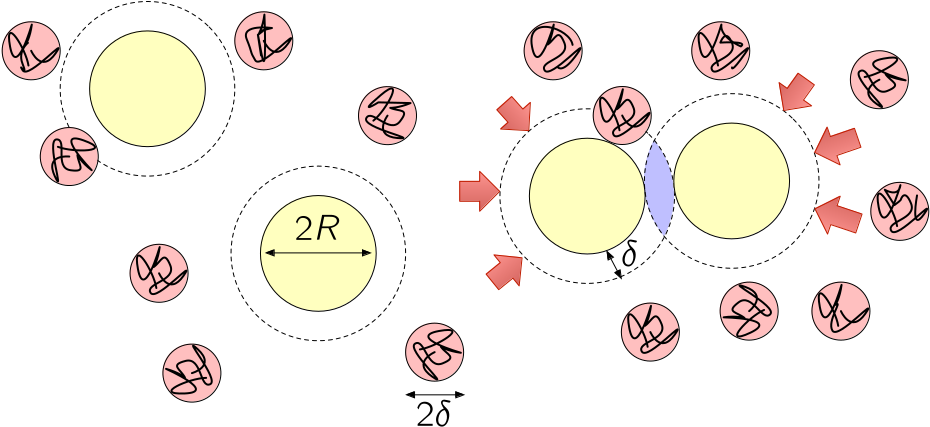
\includegraphics[keepaspectratio]{index_files/mediabag/soft-matter/figs/depletion.pdf}}

}

\caption{Mixture of colloids (yellow) and polymers (squiggly lines
inside red circles). The depletion layers are as thick as the polymer
radius (red circles) and are indicated with the dashes around the
colloids. When the two layers do not overlap, the osmotic pressure due
to the polymers on the colloids is balanced. When there is overlap,
there is a region inaccessible to the polymers (purple) and the pressure
is unbalanced, leading to aggregation.}

\end{figure}%

The simple unidimensional scenario can be extended to a more interesting
situation of hard-core colloidal particles dispersed in a medium where
other smaller, repulsive particles (e.g.~coiled polymers) are also
dispersed. It is not important atthistage to know the details of such
polymeric structures. We will ignore their internal structure and we wil
also ignore their mutual interactions. We will only consider for the
moment how they interact with the colloids and how this mediates an
interaction \emph{between} the colloids. We call these idealised
polymers \emph{penetrable hard spheres}.

This assumption yield a great simplification: the polymers, on their
own, are an ideal gas. Their chemical potnetial is given by

\begin{equation}\phantomsection\label{eq-ideal-mu}{\mu = k_BT \ln \eta_b}\end{equation}

We assume also to work in an ensemble at fixed volume \(V\), temperature
\(T\) and chemical potential \(\mu\): this is the \textbf{grand
canonical ensemble}. This means that we imagine that there is some ideal
reservoir with which we can exchange polymers in order to maintain the
chemical potential constant.

The grand potential for such ideal polymers is given by

\[\Omega = -k_BT e^{\mu/k_B T}V_{\rm accessible}\]

where \(V_{\rm accessible}\) is the accessible volume. In the absence of
the colloids, the entire volume \(V\) is accessible.

Let's image to intrudce two colloids at separation \(r\). For all
\(r> 2(R+\delta)=R_d\), the accessible volume is
\(V_{\rm accessible}^{\infty}=V-2V_{\rm exclusion}\), where \(R_d\) is
the \textbf{depletion radius} and \(V_{\rm exclusion}\) is the
inaccessible region due to the colloid-polymer interaction around each
colloid:

\[\begin{aligned}
V_{\rm exclusion}& = V_{\rm outer}-V_{\rm inner}\\
&= \dfrac{4\pi}{3}\left((R+\delta)^3-R^3\right)
\end{aligned}
\]

Changing the separation between the two colloids but maintaining
\(r>2R_d\) does not change the grand potential: there is no free energy
advantage and hence no effective interaction.

Instead, it is only when we take the colloids \emph{closer} than
\(2R_d\) that we see a free energy difference. When \(r<2R_d\) (and,
obviously, \(r>2R\)) an overlap region is formed (the lens-shaped region
of tha figur above). Its volume can be calculated simply from
geometrical considerations and it is
\begin{equation}\phantomsection\label{eq-voverlap}{
V_{\mathrm{overlap}}(r)=\dfrac{4 \pi}{3} R_d^3\left[1-\frac{3}{4} \frac{r}{R_d}+\frac{1}{16}\left(\frac{r}{R_d}\right)^3\right]
}\end{equation}

Th new accessible volume is
\[V_{\rm accessible}\prime=V-2V_{\rm exclusion}+V_{\mathrm{overlap}}\].
The interaction between the two colloids resulting from the free energy
adgvantage is called \textbf{potential of mean force} \(W(r)\). It is
expressed as

\[
\begin{aligned}
W_{\rm AO}(r) = \Omega(r)-\Omega^{\infty} & =-k_BT e^{m/k_B T}\left(V_{\rm accessible}(r)-V_{\rm accessible}(\infty)\right)\\
& = -k_BT e^{m/k_B T}\left[V-2V_{\rm exclusion}+V_{\mathrm{overlap}}(r)-(V-2V_{\rm exclusion})\right]\\
& = -k_BT e^{m/k_B T} V_{\mathrm{overlap}(r)}
\end{aligned}
\]

We can now re-use the ideal polymer chemical potential definition
Equation~\ref{eq-ideal-mu} and the gemoetrical expression for
\(V_{\mathrm{overlap}}\) in Equation~\ref{eq-voverlap} to finally write
the \textbf{Asakura-Oosawa} potential

\[
W_{\rm AO} (r) = - \dfrac{4 \pi \eta_b k_B T}{3} (R+\delta)^3\left[1-\dfrac{3}{4} \dfrac{r}{R+\delta}+\frac{1}{16}\left(\dfrac{r}{R+\delta}\right)^3\right] \quad 2R\leq r< 2R+\delta
\]

taking \(q = \delta / R\) (the polymer-to-colloid size ratio), so
\(R+\delta = R(1+q)\) and \(r/(R+\delta) = r/[R(1+q)]\) the AO potential
can also be rewritten as:

\[
W_{\rm AO}(r) = -\frac{4\pi \eta_b k_B T}{3} [R(1+q)]^3 \left[1 - \frac{3}{4} \frac{r}{R(1+q)} + \frac{1}{16} \left(\frac{r}{R(1+q)}\right)^3 \right] \quad 2R \leq r < 2R(1+q)
\]

\begin{Shaded}
\begin{Highlighting}[]
\NormalTok{\#| caption: "Asakura{-}Oosawa potential [press ctrl/cmd [ENTER] to run]"}
\NormalTok{\#| autorun: true}

\NormalTok{import numpy as np}
\NormalTok{import matplotlib.pyplot as plt}

\NormalTok{\# Parameters (change to explore)}
\NormalTok{R = 1.0           \# Colloid radius}
\NormalTok{delta = 0.2       \# Polymer radius}
\NormalTok{eta\_b = 0.1       \# Polymer concentration (dimensionless)}
\NormalTok{kBT = 1.0         \# Set kBT=1 for reduced units}

\NormalTok{\# Depletion radius}
\NormalTok{Rd = R + delta}

\NormalTok{\# r values: from contact (2R) up to 3(R+delta)}
\NormalTok{r = np.linspace(2*R, 3*Rd, 500)}

\NormalTok{def AO\_potential(r, R, delta, eta\_b, kBT):}
\NormalTok{    Rd = R + delta}
\NormalTok{    \# Only defined for 2R \textless{}= r \textless{} 2Rd}
\NormalTok{    W = np.zeros\_like(r)}
\NormalTok{    mask = (r \textgreater{}= 2*R) \& (r \textless{} 2*Rd)}
\NormalTok{    x = r[mask] / Rd}
\NormalTok{    W[mask] = {-} (4 * np.pi * eta\_b * kBT / 3) * Rd**3 * (1 {-} 0.75 * x + 0.0625 * x**3)}
\NormalTok{    return W}

\NormalTok{W\_AO = AO\_potential(r, R, delta, eta\_b, kBT)}

\NormalTok{plt.plot(r, W\_AO)}
\NormalTok{plt.gca().set(xlabel="Separation $r/R$", ylabel="$W\_\{AO\}(r)$", title="Asakura{-}Oosawa Depletion Potential")}
\NormalTok{plt.show()}
\end{Highlighting}
\end{Shaded}

\begin{tcolorbox}[enhanced jigsaw, leftrule=.75mm, bottomrule=.15mm, toprule=.15mm, colbacktitle=quarto-callout-note-color!10!white, title=\textcolor{quarto-callout-note-color}{\faInfo}\hspace{0.5em}{Force-based derivation of the AO interaction}, breakable, titlerule=0mm, opacitybacktitle=0.6, colback=white, coltitle=black, colframe=quarto-callout-note-color-frame, bottomtitle=1mm, rightrule=.15mm, toptitle=1mm, left=2mm, opacityback=0, arc=.35mm]

When the colloids are so close the polymers cannot enter the lens-shaped
region between the two colloids. This gap leads therefore to an
\emph{uniform} distribution of polymers which results in an pressure
difference: the outer polymers push the colloids together, producing an
effective attractive force. Such pressure resulting from an
uncompensated concentration gradient is called \textbf{osmotic}.

The lens-shaped overlap region between the two colloids consists of two
identical spherical caps, each subtending an angle \(\theta_0\) at the
center of the colloid. From the given geometry, the angle is such that
\[\cos\theta_0 = \dfrac{r}{2R_d}.\]

The uncompensated pressure acts on such surface.

For symmetry reasons, only the forces along the axis connecting the wto
spheres contribute to the total force. For a given angle \(\theta\) the
components is proportional to \(P\cos\theta\) where \(P\) is the
pressure exerted by the ideal gas of polymers is simply \(P=\eta_b kT\)
where \(\eta_b\) is the polymer concentration. The surface element on
which this pressure acts for a small increment \(d\theta\) is
\[dS = 2\pi R_d^2\sin\theta d\theta\]. Integrating over the range
\([0,\theta_0]\) yields the total force \(F_d\)

\[
\begin{aligned}
F_d(r) &= -2\pi \eta_b k_B T R_d^2 \int_0^{\theta_0} \sin\theta \cos\theta \, d\theta \\
&= -\pi R_d^2 \eta_b k_B T \left[1 - \left(\frac{r}{2R_d}\right)^2\right]
\end{aligned}
\]

Notice the negative sign, chosen to reflect the fact that the force is
attarctive.

Integrating the force yields the interaction potential.

\end{tcolorbox}

% Skip this GIF in PDF

\marginnote{\begin{footnotesize}

\begin{figure}[H]

{\centering \pandocbounded{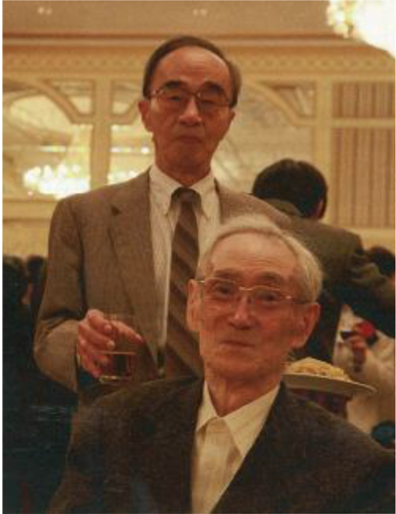
\includegraphics[keepaspectratio]{soft-matter/figs/aobirthday.png}}

}

\caption{Fumio Oosawa (front) and Sho Asakura at Oosawa's 88th birthday
(from @kurihara2021discovery )}

\end{figure}%

\end{footnotesize}}

\begin{tcolorbox}[enhanced jigsaw, leftrule=.75mm, bottomrule=.15mm, toprule=.15mm, colbacktitle=quarto-callout-note-color!10!white, title=\textcolor{quarto-callout-note-color}{\faInfo}\hspace{0.5em}{Summary of main colloid-colloid interactions}, breakable, titlerule=0mm, opacitybacktitle=0.6, colback=white, coltitle=black, colframe=quarto-callout-note-color-frame, bottomtitle=1mm, rightrule=.15mm, toptitle=1mm, left=2mm, opacityback=0, arc=.35mm]

\begin{longtable}[]{@{}
  >{\raggedright\arraybackslash}p{(\linewidth - 4\tabcolsep) * \real{0.1367}}
  >{\raggedright\arraybackslash}p{(\linewidth - 4\tabcolsep) * \real{0.6906}}
  >{\raggedright\arraybackslash}p{(\linewidth - 4\tabcolsep) * \real{0.1655}}@{}}
\toprule\noalign{}
\begin{minipage}[b]{\linewidth}\raggedright
Interaction Type
\end{minipage} & \begin{minipage}[b]{\linewidth}\raggedright
Description
\end{minipage} & \begin{minipage}[b]{\linewidth}\raggedright
Range
\end{minipage} \\
\midrule\noalign{}
\endhead
\bottomrule\noalign{}
\endlastfoot
Van der Waals & Attractive forces arising from induced dipoles between
particles. & Short-range \\
Double Layer & Electrostatic repulsion due to overlapping electrical
double layers around charged particles. & Long-range \\
DLVO & Combination of van der Waals attraction and double layer
repulsion. & Short and long range \\
Depletion & Typically attractive interactions emerging from purely
entropic interactions & Short range \\
\end{longtable}

\end{tcolorbox}

\section{Colloids as big atoms}\label{colloids-as-big-atoms}

Colloids can be viewed as ``big atoms'': they are large particles
suspended in a medium, exhibiting thermal motion and interactions in
various ways analogous to atoms, but at much larger length and time
scales. As we have seen above, the interactionsa can have statistical or
even quanto-mechanical origina, but are ultimately cast in a classical
form that is amenable to a classical treatment. At the same time, the
large scales of colloids mean that via dedicatated microscopy techniques
one is able to identify individual colloids, study theiur arrangements
in detail, and follow their dynamics.

As mentionedearlier, there is a huge variety of colloids and a vast
literature characterising their properties but also producing
theoritical and computational models.

Here we focus on the most elementary model of a colloid. The simplest
such exammple is the purely repulsive hard-sphere colloid. While an
idealisation, quasi-hard-sphere colloids can be prepared in the
laboratory by various techniques (see @royall2024colloidal ). This
includes by synthesizing a spheres of bundled polymers (you will learn
about polymers in the next chapter) such as polymethyl methacrylate
(PMMA), but also simply silica (small sphere of non-crystalline
\(\rm Si O_2\)) micron-sized beads carefully treated to screen and
minimize the electrostatic interactions that would lead to DLVO-like
contributions.

\subsection{The archetype: hard-spheres}\label{sec-hard-spheres}

A \textbf{hard-sphere} is an idealized particle model in which each
particle is represented as a perfectly rigid sphere of fixed radius
\(R\) and diameter \(\sigma=2R\). Hard spheres interact only through
excluded volume: they cannot overlap, but otherwise experience no
attraction or repulsion. The interaction potential \(U(r)\) between two
hard spheres separated by a center-to-center distance \(r\) is:

\[
U(r) = \begin{cases}
\infty & \text{if } r < \sigma \\
0 & \text{if } r \geq \sigma
\end{cases}
\]

This model captures the essential physics of \textbf{excluded volume}
which, as we said earlier, fundamentally emerges from Pauli's exclusion
principle (electrons cannot occupy the same quantum state so electronic
clouds of different atoms \emph{exclude} each other).

r U(r) 2R ∞ 0 forbidden Hard Sphere Potential

\subsubsection*{Phase behaviour of hard
spheres}\label{phase-behaviour-of-hard-spheres}
\addcontentsline{toc}{subsubsection}{Phase behaviour of hard spheres}

Since the interaction potential is only based on excluded volume, the
energy of hard spheres is trivial: it is \textbf{always zero}. A naive
interpretation of such trivial energetics may lead to conclude that
nothing interesting happens to a collection of hard spheres, since they
always are at their energy minimum (namely, zero). However, it is clear
from the earlier discussion of depletion forces that the interaction
energy is only a part of the picture for systems subject to thermal
fluctuations: indeed, for any \(T>0\), \textbf{entropic} contributions
to the free energy are always present. In the specific case of a fixed
number of hard spheres in a fixed volume, they are \emph{the only}
contribution to the free energy.

In this sense, hard-spheres are completely \textbf{entropy-driven}
system. For a collection of identical (\textbf{monodisperse}) hard
spheres the entropy is solely \textbf{configurational} and correspods to
the number of possible arrangements. This constrained only by the
accessible volume, of which we have seen an instance when considering
the depletion interactions. Notice that changing the temperature does
not really affect the statistics of the configurations: the Boltzmann
factor \(e^{U(\mathbf{r}^N)/k_BT}\) is always \(1\) for all valid
configurations. The only way we can change the state of the system is by
varying the accessible volume. For a system of \(N\) identical hard
spheres in a volume \(V\) this can only be done in two ways

\begin{itemize}
\tightlist
\item
  by adding more spheres (of the same kind)
\item
  by varying the volume V
\end{itemize}

The two routes essentially amount to varying one single parameter, which
is the \textbf{packing fraction} (also called, \emph{volume fraction})
of the system, defined as

\[\phi = N\dfrac{v_{\rm sphere}}{V} = \dfrac{\pi \sigma^6 N}{6V}\]

which can also be expressed in terms of the \textbf{number density}
\(\rho=N/V\) as \(\phi=\pi\sigma^3\rho/6\).

To change the phase behaviour of hard spheres we have a \textbf{single
control parameter}, \(\phi\) meaning that (differently from fluids like
water) we are bound to have \textbf{one-dimensional} phase diagram.

We explore the phase behaviour of hard spheres by considering different
regimes of packing fraction.

\subsubsection*{Low packing fractions}\label{low-packing-fractions}
\addcontentsline{toc}{subsubsection}{Low packing fractions}

The hard repulsion between hard spheres means that each sphere is
surrounded by an excluded volume in which the center of other spheres
cannot be placed. Since the distance of closest approach between two
spheres is \(\sigma\) such \textbf{excluded volume} per particle is
simply \(v_{\rm ex} =4\pi\sigma^3/3\) and it is much larger than the
volume pert particle \(v= V/N\). A collection of \(N\) hard spheres has
a total excluded volume \(V_{\rm ex}\neq N v_{\rm ex}\) simply because
the excluded volumes of individual particles can in general overlap, as
we saw earlier with the case of depletion.

At very low densities, most hard spheres isolated. So, in this case, we
can approximate the roral excluded volume as
\(V_{\rm ex} \rm N v_{\rm ex}\) so that the accessible volume (the
volume not occupied by the spheres) is

\[V_{\rm accessible} = V-Nv_{\rm ex}\]

We use this to perform an appropriate statistical mechanical calculation
for the Helmholtz free energy of system \(F\), which we know is purely
entropic \(F=-TS\). The partition function \(\mathcal{Z}\) is

\[
\mathcal{Z} = \frac{1}{N! \Lambda^{3N}} \int_{V_{\rm accessible}} d\mathbf{r}_1 \ldots d\mathbf{r}_N
\]

where \(\Lambda\) is the thermal de Broglie wavelength

\[\Lambda = h/\sqrt{2\pi mk_B T},\] and originates from the integration
over the Maxwell-Boltzmann disribution of momenta for particles of mass
\(m\), while \(h\) is Planck's constant.

For hard spheres, the integral is over all configurations where no two
spheres overlap (i.e., \(|\mathbf{r}_i - \mathbf{r}_j| \geq \sigma\) for
all \(i \neq j\)), and \(V_{\rm accessible}\) is the total accessible
volume. The results is that

\[\mathcal{Z} = \dfrac{(V-Nv_{\rm ex}/2)^N}{N!\Lambda^{3N}},\]

with the \(1/2\) factor coming from the fact that we avoid double
counting the excluded volume of pairs. The entropy is \[
S = k_B \ln \mathcal{Z} = k_B \left[ N \ln(V - N v_{\rm ex}/2) - \ln N! - 3N \ln \Lambda \right]
\]

From the partition function, we use Stirling's formula
\(\ln N! = N\ln N -N\) and obtain

\[
S = k_B \left[ N \ln(V - N v_{\rm ex}/2) - (N \ln N - N) - 3N \ln \Lambda \right]
\]

which reads \[
S = N k_B \left[ \ln\left( \frac{V - N v_{\rm ex}/2}{N \Lambda^3} \right) + 1 \right]
\]

The phase behaviour is encoded in the \textbf{equation of state} (the
equation that links the three thermodynamics variables \(P,T\) and
\(\phi\)). To obtain it, we calculate the pressure

\[P = -\left(\dfrac{\partial F}{\partial V}\right)_{N,T} =T\left(\dfrac{\partial S}{\partial V}\right)_{N,T}= \dfrac{k_B T }{v-v_{\rm ex}/2}\]

This expression can be simplified (do it as an exercise) to obtain the
quation of state

\[Z_{\rm comp}= \dfrac{PV}{Nk_BT}=\dfrac{1}{1-4\phi} \quad (\phi\ll 1)\]

also known as the \textbf{compressibility factor} \(Z_{\rm comp}\).
Since \(\phi\) is very small the expression is in fact

\marginnote{\begin{footnotesize}

The choice of the letter ``Z'' is unfortunate. Do not confuse the
compressibility factor with the partition function!

\end{footnotesize}}

\[Z_{\rm comp} = 1+4\phi+O(\phi^2)\]

This expression makes it apparent that the first term linear in \(\phi\)
is a \emph{correction} to the ideal gas law. This is example (to very
low order) of what is called the \textbf{virial expansion}. This, in
general takes the form

\[Z_{\rm comp}= 1 + B_2 \rho + B_3 \rho^2+ \dots\]

where \(B_2, B_3, \dots\) are the \textbf{virial coefficients} and for
systems that are not hard spheres they depend also on the temperature,
\(B_2(T), B_3(T),\dots\). They are important as they encode the effects
of \textbf{correlations}:

\begin{itemize}
\tightlist
\item
  \(B_2\) accounts for pairwise correlations (how the presence of one
  particle affects the probability of finding another nearby),
\item
  \(B_3\) for three-body correlations, and so on.
\end{itemize}

Given an interaction potential the second virial coefficient \(B_2\) can
be calculated independently from the equation state

\[
B_2(T)=-\frac{1}{2} \int_0^{\infty}\left(\exp \left(-\frac{U(r)}{k_B T}\right)-1\right) 4 \pi r^2 d r 
\]

For hard spheres this results in

\[
B_2 =  \frac{2\pi}{3} \sigma^3
\]

which is exactly what is predicted by the equation of state above, once
you recognise that \(\phi = \frac{\pi\sigma^3}{6}\rho\).

\marginnote{\begin{footnotesize}

Exercise: check this calculation.

\end{footnotesize}}

Higher-order coefficients become increasingly complex to compute and
reflect more complex many-body corelations that can be established even
if the interaction potential is purely twobody (as in the case of hard
spheres). The higher order coefficients become mor eand more important
as the packing fraction is increased. Eventually something surprising
occurs at a sufficiently high volume fraction.

\subsubsection*{Dense packing: metastability and
crystalisation}\label{dense-packing-metastability-and-crystalisation}
\addcontentsline{toc}{subsubsection}{Dense packing: metastability and
crystalisation}

As we increase the packing fraction, the accessible (free) volume
reduces rapidly. At some point, disordered packing of spheres are so
tightly packed that thermal motion becomes extremely inefficient or even
impossible. Such disordered (\textbf{random}) packing of spheres are
described as \textbf{jammed}: they are so densely packed that they are
no longer behaving like a fluid but they instead display some of the
rigidity that we typically associate with solids. Such jammed
configurations are indeed examples of \textbf{amorphous solids}. We will
explore them more in detail in the chapter dedicated to arrested
systems.

It is important to note, however, that the disordered packing at high
volume fractions are not minima of the free energy. The densest possible
packing of hard spheres is achieved by arranging them in a crystalline
lattice. In three dimensions, the densest packings are the face-centered
cubic (FCC) and hexagonal close-packed (HCP) structures, both of which
have a maximum packing fraction of

\[
\phi_{\text{max}} = \frac{\pi}{3\sqrt{2}} \approx 0.74
\]

This means that, at most, about 74\% of the available volume can be
filled by the spheres, with the remainder being empty space. This result
was conjectured by Kepler in 1611 and proved rigorously only in 1998
(the \href{https://en.wikipedia.org/wiki/Kepler_conjecture}{Kepler
conjecture}).

In contrast, \textbf{random close packing} (the densest disordered
arrangement of spheres) yields a lower packing fraction, typically
around \(\phi_{\text{rcp}} \approx 0.64\). Notice that this value is
approximate and variations can be observed (due to randomness and, more
importantky, to the method by which such packing are reached, i.e.~the
\emph{compression protocol}). This means that the only way to compress
spheres at very high packing has to lead (\emph{spontaneously}) to the
formation of crystals. We can indeed imagine to perform the following
experiment:

\begin{itemize}
\tightlist
\item
  prepare a disordered assembly of colloidal hard spheres
\item
  compress them gradually to high and higher packing fraction, taking
  care to monitor the systems so that time correlations decay and the
  system is at thermal equilibrium
\item
  measure the resulting packing fraction
\end{itemize}

Experiments of this sort have been performed historically, leveraging
for example the \textbf{slow sedimentation} of colloids, which on long
time scales leads to the accumulation of dense packings of spheres. Such
experiments reveal that beyond the so-called \textbf{freezing packing
fraction} \(\phi_{f} 0.494\) the system spontaneously forms small
regions of crystals mixed with the fluid. At a the high \textbf{melting
packing fraction} \(\phi_{m}=0.545\) the entirety of the system is then
crystalline and its optical properties consequently change.

\begin{figure}[H]

{\centering \pandocbounded{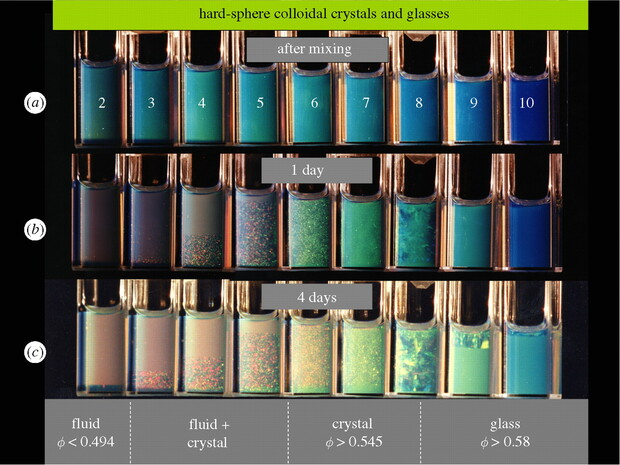
\includegraphics[keepaspectratio]{soft-matter/figs/rsta20090181f01.jpg}}

}

\caption{Phase behaviour of hard-sphere colloids from @pusey2009hard}

\end{figure}%

A simple \textbf{cell model} can help us rationalise what is taking
place. When the spheres are packed within their FCC cell, they can move
very little beyond their own diameter \(\sigma\). Assume that the volume
per particle again is \(v\) and the (geometrically consrained) close
packed volume is \(v_{cp}\).

The maximum dispalcement is \[
\delta=\frac{\sigma}{\sqrt{2}}\left(\left(\frac{v}{v_{c p}}\right)^{1 / 3}-1\right)
\] The corresponding free volume is then
\(v_f=\frac{4 \pi}{3} \delta^3\) from which we can calculate the entropy

\[
S = -N k_B T \ln \left(v_f / \Lambda^3\right)
\]

and the resulting pressure

\[
P=\frac{N k_B T}{v_{c p}} \frac{\left(v / v_{c p}\right)^{-2 / 3}}{\left(v / v_{c p}\right)^{1 / 3}-1}
\]

Rearranging and expressing everything in terms of packing fraction
\(\phi = \dfrac{\pi\sigma^3}{6v}\) yields

\[
Z_{\rm comp}=\frac{1}{1-\left(\phi / \phi_{c p}\right)^{1 / 3}}
\]

What is noteable here is that the expression we have obtained is a
completely different functional form compared to the low density fluid
regime. Thisis indicative of a \textbf{discontinuous},
\textbf{first-order} phase transition between the fluid and the
crystalline phases. First order phase transitions are characterised by
coexisting regions where the system can be found in partial fluid and
partial crystaline state, as illustrated in the experiments above. This
also means that we can prepare a disordered packing at very high
density: this will not be its equilibrium state (global minimum of the
free energy), but will still be stable for some (finite) time. This
\emph{local equilibrium state} is called a *\textbf{metastable state}.

\begin{figure}[H]

{\centering \pandocbounded{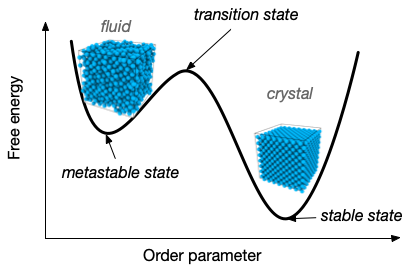
\includegraphics[keepaspectratio]{soft-matter/figs/metastable.png}}

}

\caption{Schematic free energy for hard spheres compressed at high
pressures: the fluid branch becomes metastable and the free enrgy
minimum is located in the crystal phase}

\end{figure}%

But where does the free energy advantage of the crystal over the
disrodered fluid come from? From the discussion above the answer is
obvious: crystals can accommodate higher packings, meaning that they use
the availale volume more efficiently. This in fact means that (on
average) every hard sphere has more available volume if it arranged in
the crystalline state compared to the fluid phase: the increased volume
(available for thermal fluctuations and random particle displacements)
is translated into an \textbf{increased entropy}. So, in fact the
ordered, crystalline state has overall a higher entropy than the
disordered fluid. This is important instance in which the conventional
storytelling, where entropy is just \textbf{disorder}, simply does not
hold. As we have seen with depletion forces earlier, entropy can lead to
structure: in the case of hard spheres, it si the only mechanism leading
to structure, and such structure is the most orderly one can think of:
long-range, crystalline order.

The video below shows instead the results of a Monte-Carlo simulation at
packing \(\phi=0.493\) for a small system of 32 particles. Small systems
have enhanced fluctuations, and since the overal packing fraction is
very close to the freezing line, we see spontaneous freezing and
unfreezing of the small system (wait until second 14 in the movie).

\url{figs/melt_freeze.mp4}

In conclusion, colloidal hard spheres have a one-dimensional phase
diagram, that depends only on the packing fraction but with various
distinct phases

\begin{figure}[H]

{\centering \pandocbounded{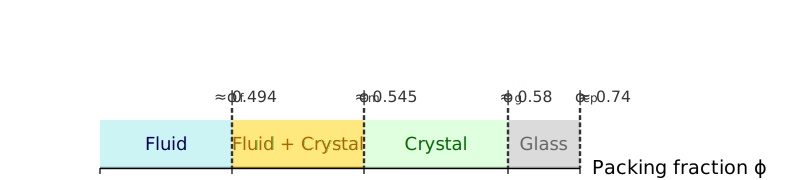
\includegraphics[keepaspectratio]{index_files/mediabag/soft-matter/figs/hard-sphere-diag.pdf}}

}

\caption{Hard-spheres phase diagram}

\end{figure}%

\subsection{Beyond hard-spheres: simple
liquids}\label{beyond-hard-spheres-simple-liquids}

A \textbf{simple liquid} is a system of particles interacting via
short-range, spherically symmetric (isotropic) pair potentials. The most
common model is the \textbf{Lennard-Jones (LJ) potential}, which
captures both the short-range repulsion (due to Pauli exclusion) and
longer-range van der Waals attraction:

\[
U_{\mathrm{LJ}}(r) = 4\epsilon \left[ \left( \frac{\sigma}{r} \right)^{12} - \left( \frac{\sigma}{r} \right)^6 \right]
\]

where \(\epsilon\) sets the depth of the potential well (interaction
strength) and \(\sigma\) is the particle diameter (distance at which
\(U=0\)). The \(r^{-12}\) term models steep repulsion, while \(r^{-6}\)
describes the attractive tail.

The Lennard-Jones fluid exhibits rich phase behavior: at low
temperatures and densities, it forms a gas; at intermediate conditions,
a liquid; and at high densities, a solid. The LJ model is widely used to
study atomic and molecular liquids, and serves as a reference for
understanding real fluids and their phase transitions.

In the phase diagram below these different phases have been highlighted.
It is clear that, compared to hard spheres which only display a fluid
and a crystalline solid phase, systems like the Lennard-Jones fluid
display an additional phase, the \textbf{liquid}. This phase emerges
from the presence of the attractive well in the interaction potential.
This allows for short-range attractive interactions that case a region
of teh phase diagram in the save class of universality of the
\hyperref[sec:models]{\textbf{Ising model}} and the
\href{../phase-transitions/lattice-gas.qmd}{\textbf{lattice gas}}.

\begin{figure}[H]

{\centering \pandocbounded{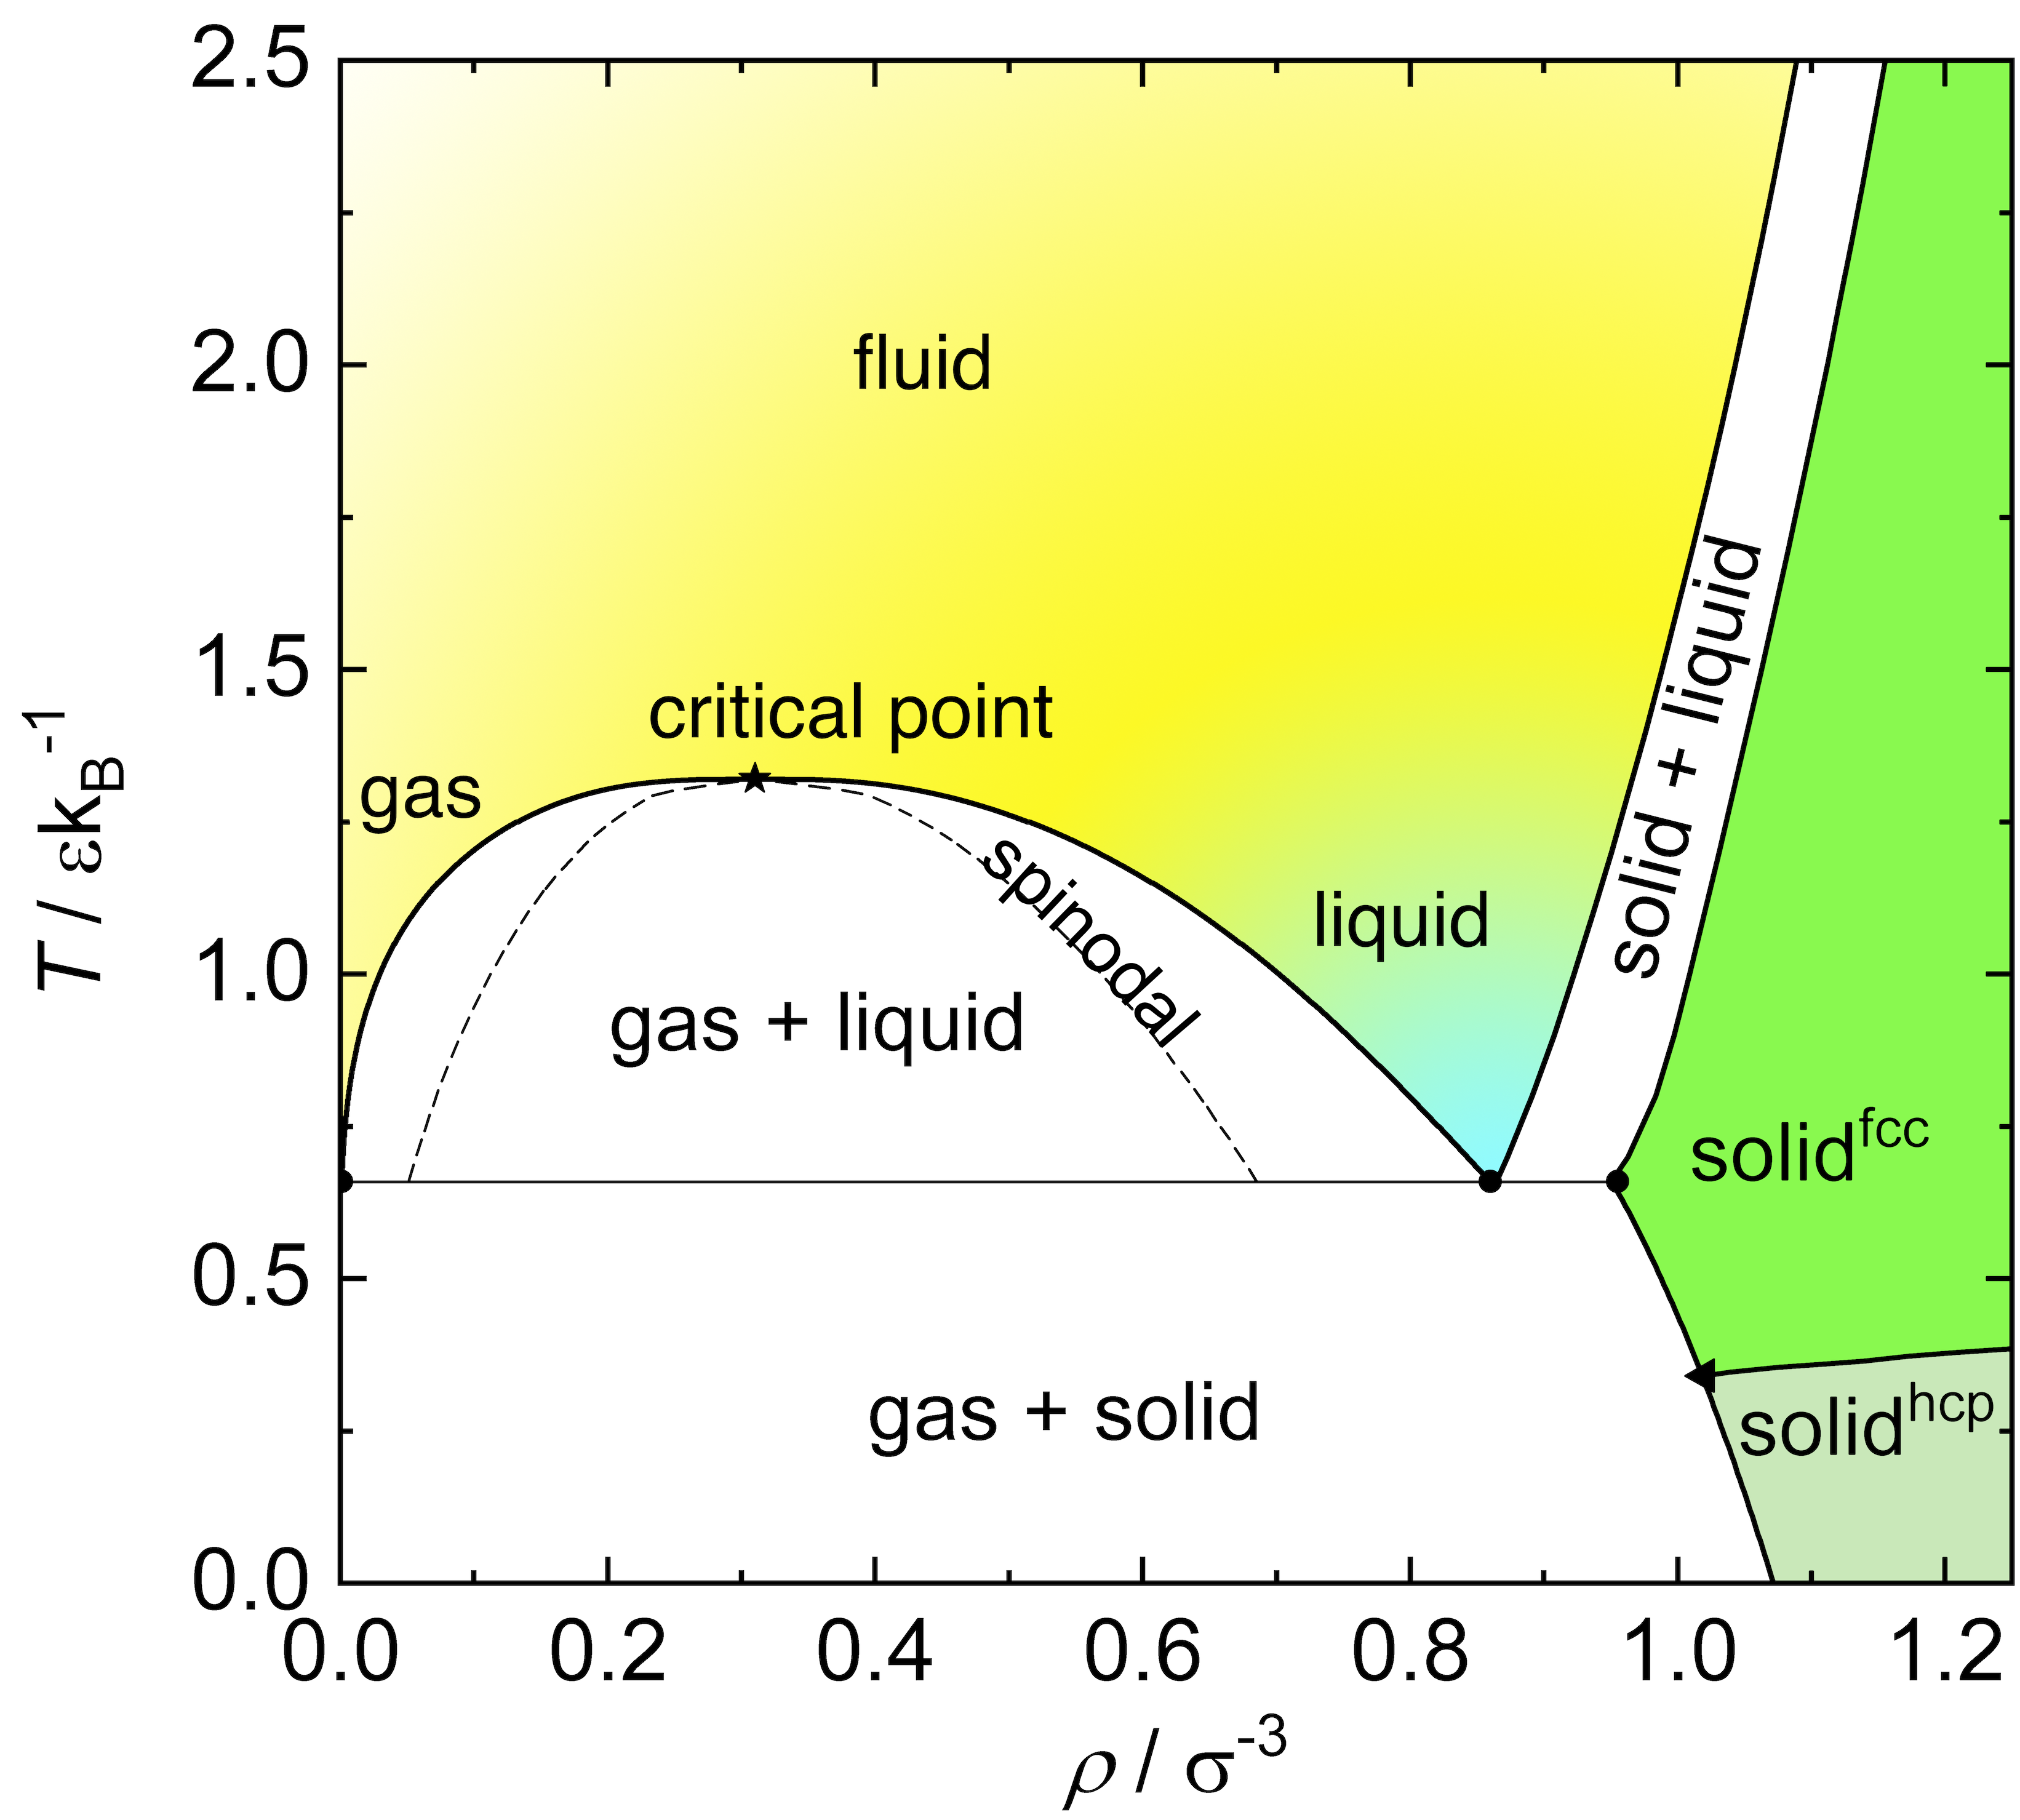
\includegraphics[keepaspectratio]{soft-matter/figs/LJPhaseDiagram.png}}

}

\caption{Phase diagram of the Lennard-Jones Fluid, adapted from
Wikimedia.}

\end{figure}%

The Lennard-Jones interaction has already been designed to model noble
gases (e.g.~Argon) but has over time been used to model many other
systems due to its simplicity and computational convenince: in
particular it is used tor construct coarse-grained models of
macromolecules, as well as colloids and nanoparticles. It belongs to a
wider class of, classical, effective \textbf{pair-wise} interaction
models actensively used to claculate properties and phase diagrams of a
variety of condensed matter systems. This are useful because they allow
one to, for example, long molecular simulations that are normally
unreachable when considering atomistics and electronic density
calculations.

The following table provides you with a few example potentials and their
functional forms:

\begin{longtable}[]{@{}
  >{\raggedright\arraybackslash}p{(\linewidth - 4\tabcolsep) * \real{0.1373}}
  >{\raggedright\arraybackslash}p{(\linewidth - 4\tabcolsep) * \real{0.5425}}
  >{\raggedright\arraybackslash}p{(\linewidth - 4\tabcolsep) * \real{0.3203}}@{}}
\toprule\noalign{}
\begin{minipage}[b]{\linewidth}\raggedright
Potential Name
\end{minipage} & \begin{minipage}[b]{\linewidth}\raggedright
Mathematical Form
\end{minipage} & \begin{minipage}[b]{\linewidth}\raggedright
Typical Systems/Features
\end{minipage} \\
\midrule\noalign{}
\endhead
\bottomrule\noalign{}
\endlastfoot
Lennard-Jones (LJ) &
\(U(r) = 4\epsilon \left[ \left( \frac{\sigma}{r} \right)^{12} - \left( \frac{\sigma}{r} \right)^6 \right]\)
& Simple atomic fluids, coarse-grained molecular interactions \\
Hard Sphere &
\(U(r) = \begin{cases} \infty & r < \sigma \\ 0 & r \geq \sigma \end{cases}\)
& Colloids, granular materials, excluded volume \\
Yukawa (Screened Coulomb) & \(U(r) = \epsilon \frac{e^{-\kappa r}}{r}\)
& Charged colloids, plasmas, electrolytes \\
Dipolar &
\(U(r) = \frac{\mu_0}{4\pi} \frac{\mu_1 \mu_2}{r^3} (1 - 3\cos^2\theta)\)
& Magnetic colloids, polar molecules \\
\end{longtable}

\section{Characterisation of colloidal
systems}\label{characterisation-of-colloidal-systems}

When looking at colloidal systems, we typically focus on two main
aspects of their physics:

\begin{itemize}
\tightlist
\item
  their \textbf{structural features}, chracterised by the
  \textbf{spatial} correlations between their constituents
\item
  their \textbf{dynamical features}, characterised by the mobility of
  single particles or groups of particles.
\end{itemize}

Here below, we briefly account of some main approaches to characterise
these two dimensions.

\subsection{Structural properties: the radial distribution
function}\label{structural-properties-the-radial-distribution-function}

Structural features of disordered (but also ordered) systems are
described in terms of \textbf{correlation functions}. The underlying
idea is that we are provided with an ensemble of stochastic variables
(the positions of the colloids) which have a characteristic spatial
distribution. for \(N\) particles we have an N-body probability
distribution function \(\rho_N(\mathbf{r}^N)\) which contains all the
necessary statistical mechanical information to describe the
thermodyanmics of the system. However, this is very difficult to access
directly. In experiments or theoretical calculations we typically only
have access to some lower order \emph{marginalisation} of the
distribution, in terms of few-body distributions.

One of the simplest assumptions we can make when we describe a system is
that its potential energy is expressed in terms of purely pairwise
additive potential, meaning that

\[ U_N (\mathbf{r}^N)=\sum_{i=1}^{N-1}\sum_{j=i+1}^N V(r_ij) = \dfrac{1}{2}\sum_{i\neq j}V(r_{ij})\]

where \(V(r_{ij})\) is the pairwise, radial interaction potential that
only depends on the distance between particle centres
\(r_{ij} = \mathbf{r}_i-\mathbf{r}_j\).

For system with pariwise interactions, the natural spatial correlation
function is a twobody correlation \(g(\mathbf{r}_i, \mathbf{r}_j)\),
where \(\mathbf{r}_i\) and \(\mathbf{r}_j\) are two randomly chosen
particles. In the case of non-crystalline, disordered systems the
corrlation function has to be

\begin{itemize}
\tightlist
\item
  translationally invariant , so that it only depends on the difference
  \(\mathbf{r}_i-\mathbf{r}_j\)
\item
  rotationally invariant, so that there is no angular component and
  hence only the distance \(r_{ij} =| \mathbf{r}_i-\mathbf{r}_j|\)
  matters
\end{itemize}

This function \(g(r)\) is called the \textbf{radial distribution
function} and plays a crucial role in the characterisation of fluids,
crystals, glasses and much more. For system with twobody interactions
only, it contains in principle all the thermodynamic information
necessary to reconstruct the free energy, as one can write

\[
\frac{F_{\mathrm{ex}}}{k_B T}=2 \pi \rho N \int_0^{\infty}[g(r) \ln g(r)-g(r)+1] r^2 d r+\frac{\rho N}{2 k_B T} \int V(r) g(r) d^3 r
\] where the first term represent the entropic contributions and the
second term represents the energetic contribution.

But how is it calculated? very simply. You can think of constructing a
histogram of the distances between all of the particles and suitably
normalising such histogram by the density of the system. Mathematically
this reads as

\[
g(r) = \frac{1}{\rho N} \left\langle \sum_{i=1}^N \sum_{j \neq i} \delta(|\mathbf{r}_i - \mathbf{r}_j| - r) \right\rangle
\]

where \(\rho = N/V\) is the number density, and the angle brackets
denote an ensemble average and \(\delta\) is a Dirac delta function.

\begin{itemize}
\tightlist
\item
  For an \textbf{ideal gas}, \(g(r) = 1\) everywhere (no correlations).
\item
  For \textbf{hard spheres}, \(g(r) = 0\) for \(r < \sigma\) (no
  overlap), and \(g(r)\) shows oscillations at higher \(r\) due to
  packing effects.
\end{itemize}

Notice that the radial distribution function is an instance of the more
general class of pair-wise correlations that have been introduced
earlier, see Section~\ref{sec-correlations} and it is paired with its
reciprocal space Fourier transform, the \textbf{structure factor}:

\[
S(k) = 1 + \rho \int \left[ g(r) - 1 \right] e^{-i \mathbf{k} \cdot \mathbf{r}} d\mathbf{r}
\]

For isotropic systems, this reduces to:

\[
S(k) = 1 + 4\pi \rho \int_0^\infty r^2 [g(r) - 1] \frac{\sin(kr)}{kr} dr
\]

Experimentally, on can measure \(S(k)\) can be measured using scattering
techniques or \(g(r)\) via direct imaging in colloidal systems. They
provide insight into short-range order, local structure, and phase
transitions in soft matter.

\begin{tcolorbox}[enhanced jigsaw, leftrule=.75mm, bottomrule=.15mm, colback=white, colframe=quarto-callout-important-color-frame, arc=.35mm, breakable, rightrule=.15mm, left=2mm, opacityback=0, toprule=.15mm]
\begin{minipage}[t]{5.5mm}
\textcolor{quarto-callout-important-color}{\faExclamation}
\end{minipage}%
\begin{minipage}[t]{\textwidth - 5.5mm}

The radial distribution function \(g(r)\) has two possible
interpretations

\begin{itemize}
\tightlist
\item
  It represents the probability density of finding a particle at
  distance \(r\) away from a reference particle \emph{relative} to the
  probability density of an idela gas at the same number density.
\item
  If a given refernce particle is taken at the origin, then the local
  average density at distance \(r\) is \(\rho g(r)\).
\end{itemize}

\end{minipage}%
\end{tcolorbox}

Here below we show two codes to calculate the radial distribution
fucntion for an ideal gas (which is trivial) and then for an assembly of
hard spheres

\begin{Shaded}
\begin{Highlighting}[]
\NormalTok{\#| caption: "Radial distribution function of an ideal gas [press ctrl/cmd [ENTER] to run]"}
\NormalTok{\#| autorun: true}
\NormalTok{import numpy as np}
\NormalTok{import matplotlib.pyplot as plt}

\NormalTok{\# Parameters}
\NormalTok{N = 500      \# number of points, change this to check convergence}
\NormalTok{L = 10.0     \# box size}
\NormalTok{bins = 50    \# number of bins}

\NormalTok{\# Generate random points (ideal gas)}
\NormalTok{positions = np.random.uniform(0, L, size=(N, 3))}

\NormalTok{def radial\_distr(positions, L):}
\NormalTok{    N = len(positions)}
    
\NormalTok{    \# Compute all pairwise distances with PBC}
\NormalTok{    diff = positions[:, np.newaxis, :] {-} positions[np.newaxis, :, :]}
\NormalTok{    diff = diff {-} L * np.round(diff / L)}
\NormalTok{    dists\_matrix = np.sqrt(np.sum(diff**2, axis={-}1))}
    
\NormalTok{    \# Get upper triangular distances (each pair counted once)}
\NormalTok{    i, j = np.triu\_indices(N, k=1)}
\NormalTok{    dists = dists\_matrix[i, j]}
    
\NormalTok{    \# Create histogram}
\NormalTok{    r\_max = L/2}
\NormalTok{    r\_edges = np.linspace(0, r\_max, bins+1)}
\NormalTok{    hist, \_ = np.histogram(dists, bins=r\_edges)}
\NormalTok{    r\_centers = 0.5 * (r\_edges[:{-}1] + r\_edges[1:])}
    
\NormalTok{    \# Calculate g(r) with correct normalization}
\NormalTok{    rho = N / L**3  \# number density}
\NormalTok{    dr = r\_edges[1:] {-} r\_edges[:{-}1]  \# bin widths}
    
\NormalTok{    \# Volume of spherical shell}
\NormalTok{    shell\_volumes = 4 * np.pi * r\_centers**2 * dr}
    
\NormalTok{    \# For each particle, expected number of neighbors in shell = rho * shell\_volume}
\NormalTok{    \# Total expected pairs in shell = N * rho * shell\_volume / 2 }
\NormalTok{    \# (divide by 2 because we count each pair once)}
\NormalTok{    expected\_pairs = N * rho * shell\_volumes / 2}
    
\NormalTok{    \# g(r) = actual\_pairs / expected\_pairs}
\NormalTok{    g\_r = hist / expected\_pairs}
    
\NormalTok{    return r\_centers, g\_r}

\NormalTok{r, g = radial\_distr(positions, L)}
\NormalTok{plt.plot(r, g, \textquotesingle{}b{-}\textquotesingle{}, drawstyle="steps{-}mid")}
\NormalTok{plt.axhline(y=1, color=\textquotesingle{}r\textquotesingle{}, linestyle=\textquotesingle{}{-}{-}\textquotesingle{}, alpha=0.7, label=\textquotesingle{}Ideal gas (g(r)=1)\textquotesingle{})}
\NormalTok{plt.xlabel("r")}
\NormalTok{plt.ylabel("g(r)")}
\NormalTok{plt.gca().set(xlim=(0, L/2),ylim=(0,2))}
\NormalTok{plt.legend()}
\NormalTok{plt.show()}
\end{Highlighting}
\end{Shaded}

We can compare this with arrangements of hard spheres

\begin{Shaded}
\begin{Highlighting}[]
\NormalTok{\#| caption: "Radial distribution function for a hard sphere configuration [press ctrl/cmd [ENTER] to run]"}
\NormalTok{\# now try with hard spheres, using a custom libarry you will find in the course pages}
\NormalTok{from src import hardspheres}

\NormalTok{sigma = 1.0}
\NormalTok{L = 5.*sigma \#take a small value}
\NormalTok{phi = 0.2 \# packing fraction}
\NormalTok{N = int(phi/(np.pi/6*sigma**3)*L**3)}

\NormalTok{\#  we run Monte{-}Carlo simulations of hard{-}spheres on the fly }
\NormalTok{freq = 5}
\NormalTok{nsteps = 100*N}
\NormalTok{trajectory, acceptance = hardspheres.Monte\_Carlo\_traj(N,L, sigma, nsteps,freq)}
\NormalTok{gs = []}
\NormalTok{for positions in trajectory:}
\NormalTok{    \_r, \_g = radial\_distr(positions, L)}
\NormalTok{    gs.append(\_g)}
\NormalTok{plt.plot(r, np.mean(gs,axis=0), \textquotesingle{}b{-}\textquotesingle{}, label=rf"Hard spheres, rf$\textbackslash{}phi=\{phi\}$")}
\NormalTok{plt.set(xlabel="r", ylabel="g(r)", ylim= (0,2))}
\NormalTok{plt.legend()}
\NormalTok{plt.show()}
\end{Highlighting}
\end{Shaded}

The radial distribution function is the central object of much of
\textbf{liquid state theory}, which aims to predict the shape of the
correlation functions (such as \(g(r)\)) from the sole knowledge of the
interaction potential between the elementary particles (see
@santos2016concise for a gentle introduction to the topic). In
particular, one can imagine the correlations between two particles \(1\)
and \(2\) in a fluid to have two possible origins

\begin{itemize}
\tightlist
\item
  a \textbf{direct} correlation between the two particles, mediated by
  direct interactions (e.g.~collisions) between 1 and 2.
\item
  an \textbf{indirect correlation}, mediated by other particle sin the
  fluid
\end{itemize}

The \(g(r)\) contains both direct and indirect correlations. We can
assume that a suitable function \(c(r)\) exists to express the direct
correlations. In such case, for twobody interactions, we cna write a
hierarchy of equations via a central result of liquid state theory, the
\textbf{Ornestein-Zernicke} (OZ) equation

\begin{equation}\phantomsection\label{eq-oz}{
h\left(r_{12}\right)=c\left(r_{12}\right)+\rho \int c\left(r_{13}\right) h\left(r_{32}\right) d \mathbf{r}_3
}\end{equation}

where we defined the total correlation function as \(h(r)=g(r)-1\). The
OZ equation is an integral equation. In Fourier space (assuming the
isotropicity of a fluid) it becomes an algebraic equation \[
\tilde{h}(k)=\frac{\tilde{c}(k)}{1-\rho \tilde{c}(k)}
\] Since both \(h(r)\) and \(c(r)\) an additional relationship is known
called a \textbf{closure}. These constructed through phsyical arguments.
A common one is the so-caled Percus-Yevick closure

\[
c(r)=[1+h(r)]\left[1-e^{\beta U(r)}\right]
\] where the pairwise interaction enters explicitly.

Solving the OZ equation with the Percus-Yevick closure produces
realistic radial distribution functions in a wide range of packing
fractions for hard spheres.

\subsection{Dynamics: single vs collective
displacements}\label{dynamics-single-vs-collective-displacements}

We have seen
\href{../phase-transitions/Brownian-and-Langevin-dynamics.qmd}{earlier}
that if we are given a number of particles evolving microscopically
according to the Langevin equation of drag \(\gamma\) and zero-mean
noise \(\eta\)

\[
m \frac{d \vec{v}}{d t}=-\gamma\vec{v}+\vec{\eta}(t)
\]

then an \emph{ensemble} of independent particles will follow the
\textbf{diffusion equation}:

\[\frac{\partial \rho(\mathbf{r}, t)}{\partial t} = D \nabla^2 \rho(\mathbf{r}, t) \]

where \(\rho(\mathbf{r},t)\) is the probability of finding a particle at
position \(\mathbf{r}\) at time \(t\) with diffusivity \(D\). The
diffusivity \(D\) is related to the microscopic Langevin equation
parameters via the fluctuation-dissipation relation (or Einstein
relation) \[
D = \frac{k_B T}{\gamma}
\] where \(k_B\) is Boltzmann's constant, \(T\) is temperature, and
\(\gamma\) is the friction (drag) coefficient.

It is easy to show (see below) that in 1 dimension the general solution
is

\[
\rho(x, t) = \frac{1}{\sqrt{4\pi D t}} \exp\left(-\frac{x^2}{4Dt}\right)
\]

\begin{tcolorbox}[enhanced jigsaw, leftrule=.75mm, bottomrule=.15mm, toprule=.15mm, colbacktitle=quarto-callout-note-color!10!white, title=\textcolor{quarto-callout-note-color}{\faInfo}\hspace{0.5em}{Solution of the diffusion equation using Laplace transform}, breakable, titlerule=0mm, opacitybacktitle=0.6, colback=white, coltitle=black, colframe=quarto-callout-note-color-frame, bottomtitle=1mm, rightrule=.15mm, toptitle=1mm, left=2mm, opacityback=0, arc=.35mm]

The 1D diffusion equation is: \[
\frac{\partial \rho(x, t)}{\partial t} = D \frac{\partial^2 \rho(x, t)}{\partial x^2}
\]

Suppose the initial condition is a delta function at the origin: \[
\rho(x, 0) = \delta(x)
\]

Take the Laplace transform in time: \[
\tilde{\rho}(x, s) = \int_0^\infty \rho(x, t) e^{-st} dt
\]

The Laplace transform of the time derivative: \[
\mathcal{L}\left[\frac{\partial n}{\partial t}\right] = s\tilde{\rho}(x, s) - \rho(x, 0)
\]

So the transformed equation is: \[
s\tilde{\rho}(x, s) - \delta(x) = D \frac{\partial^2 \tilde{\rho}(x, s)}{\partial x^2}
\]

Rearrange: \[
D \frac{\partial^2 \tilde{\rho}}{\partial x^2} - s\tilde{\rho} = -\delta(x)
\]

For \(x \neq 0\), the homogeneous equation: \[
D \frac{\partial^2 \tilde{\rho}}{\partial x^2} - s\tilde{\rho} = 0
\]

General solution: \[
\tilde{\rho}(x, s) = A e^{-\lambda |x|}, \quad \lambda = \sqrt{\frac{s}{D}}
\]

The delta function at \(x=0\) gives a discontinuity in the derivative:
\[
\left.\frac{\partial \tilde{\rho}}{\partial x}\right|_{x=0^+} - \left.\frac{\partial \tilde{\rho}}{\partial x}\right|_{x=0^-} = -\frac{1}{D}
\]

Compute derivatives: \[
\frac{\partial \tilde{\rho}}{\partial x} = -A \lambda \, \text{sgn}(x) e^{-\lambda |x|}
\]

So at \(x=0^+\): \(-A\lambda\), at \(x=0^-\): \(A\lambda\). The jump is
\(-2A\lambda\).

Set equal to \(-1/D\): \[
-2A\lambda = -\frac{1}{D} \implies A = \frac{1}{2D\lambda}
\]

So: \[
\tilde{\rho}(x, s) = \frac{1}{2D\lambda} e^{-\lambda |x|} = \frac{1}{2\sqrt{Ds}} e^{-|x|\sqrt{\frac{s}{D}}}
\]

Invert the Laplace transform (using tables or convolution theorem): \[
\rho(x, t) = \frac{1}{\sqrt{4\pi D t}} \exp\left(-\frac{x^2}{4Dt}\right)
\]

This is the fundamental solution (Green's function) of the diffusion
equation.

\end{tcolorbox}

The diffusion equation can also be read as a simple consequence of two
requirements:

\begin{itemize}
\item
  continuity of the distribution of mass (no mass is lost during the
  transport), as expressed in the \textbf{continuity equation} \[
  \frac{\partial \rho(\mathbf{r}, t)}{\partial t} + \nabla \cdot \mathbf{J}(\mathbf{r}, t) = 0
  \] where the divergence \(\nabla \cdot \mathbf{J}(\mathbf{r}, t)\)
  represents the net outflow of particles from a given region due to the
  flux \(\mathbf{J}\).
\item
  the flux of particles is assumed to be proportional to the gradient in
  the density (or concnetration of the particles). This can be taken as
  an empirical assumption, a reasonable approximation (i.e.~a
  perturbative approach) or a consequence of underlying Brownian
  dynamics. It is known as Fick's law:
\end{itemize}

\[
\mathbf{J}(\mathbf{r}, t) = -D \nabla \rho(\mathbf{r}, t)
\]

The diffusivity constant \(D\) is therefore central for the diffusion.
It is possible to link the microscopic motion of the particles to the
collective behaviour of the density distribution \(\rho(x,t)\) by
exploting the connection provided bt the \textbf{mean squared
displacement}, which is simply the variance of the distributione
\(\rho(x,t)\) at time \(t\).

As discussed earlier, in \(d\) dimensions this is equal to
\[\langle r(t)^2\rangle-\langle r(t)\rangle^2 = 2d D t\]

Hence, measuring the average squared displacements is sufficient to
recover the diffusivity and to reconstruct the distribution.

\subsubsection{Diffusion and
interactions}\label{diffusion-and-interactions}

We have up to now considered the dilute (or non-nteracting) limit, where
collisions between the colloids are ignored. Let's now consider instead
simple colloids (again, hard spheres) and their dynamics.

We are interested in the mean squared displacement
\(\left\langle r^{2}(t)\right\rangle\) as a function of time for
different volume fractions. At low volume fractions, the particles
undergo Brownian motion (random-walk diffusion) due to collisions with
liquid molecules. The mean squared displacement (in three dimensions) is
\[\left\langle\underline{r}^{2}(t)\right\rangle=6 D_{0} t\] where the
meaning of the subscript 0 will be apparent shortly.

For sufficiently dense hard spheres (e.g.~above \(\phi \sim 0.3\)),
however, different regimes are observed. At short times the particles
diffuse with the short time (self) diffusion constant \(D_{s}\). This is
determined from the short time limit and is smaller than the \(D_{0}\)
measured for \(\phi \rightarrow 0\). The motion of the particles (self
diffusion) is still driven by collisions with the liquid molecules, but
in addition the interactions between particles become significant.

While the particles are diffusing in their cages formed by their
neighbours, the hydrodynamic interaction with the neighbours,
transmitted through flows in the liquid, causes slowing down relative to
the free diffusion at low concentrations. At intermediate times the
particles encounter the neighbours and the interactions slow the motion
down. To make further progress, the particle has to break out of the
cage formed by its neighbours. Now the particles experience a further
interaction, direct interactions (hard-sphere interactions), in addition
to the hydrodynamic interactions. The long-time and long-ranged movement
is also diffusive, i.e.~we still have
\[\langle r^{2}(t)\rangle \propto t\] when the particles undergo
large-scale random-walk diffusion through many cages.

However, the motion is further slowed and a smaller diffusion constant
relative to the motion in the short time limit is observed, the long
time (self) diffusion constant \(D_{L}\).

The slowing down due to collisions eventually dominates the ohysics of
hard spheres at high densities. This is more broadly true also for
generic dense colloidal suspensions, where the short range interactions
dominate on other mechanisms of motion (including the hydrodynamics).
Eventually, for very dense packings one observes the emergence of a new
physical regime where relaxation becomes anomalous and non-diffusive:
this is the glassy regime, which we will revisit in a following chapter.

\subsection{Stokes-Einstein relation}\label{stokes-einstein-relation}

Suppose that the particles are subjected to an external force F in the x
direction, e.g.~gravity. In thermal equilibrium the Maxwell-Boltzmann
distribution is valid, i.e.~the particle density \(n(x)\) is given by

\[
n(x)=n_{0} \exp \left(-U(x) / k_{B} T\right)=n_{0} \exp \left(-F x / k_{B} T\right)
\]

where we assumed a constant force \(F\) in the last equation. In the
case of gravity \(F=m_{B} g\) with \(m_{B}\) the buoyant mass. \(n(x)\)
results from the balance between the motion of the particles due to the
external force setting up a concentration gradient, and the resultant
diffusion given by Fick's law.

\begin{Shaded}
\begin{Highlighting}[]
\NormalTok{// | echo: false}
\NormalTok{\{}
\NormalTok{  const width = 600;}
\NormalTok{const height = 400;}
\NormalTok{const numCircles = 300;}

\NormalTok{let temperature = 300;    // Arbitrary scale}
\NormalTok{let viscosity = 0.02;     // Arbitrary scale}
\NormalTok{const particleRadius = 5; // pixels}
\NormalTok{let timeStep = 1;}

\NormalTok{const kB = 1; // reduced units}
\NormalTok{let gravityFactor = 0.1;}
\NormalTok{let gravity = 10 * gravityFactor;}

\NormalTok{// Compute damping as velocity decay per timestep (Langevin friction)}
\NormalTok{function computeDamping(viscosity, radius, dt) \{}
\NormalTok{  const gamma = 6 * Math.PI * viscosity * radius; // friction coeff}
\NormalTok{  return Math.exp({-}gamma * dt);}
\NormalTok{\}}

\NormalTok{let damping = computeDamping(viscosity, particleRadius, timeStep);}

\NormalTok{// Create SVG}
\NormalTok{const svg = d3.create("svg")}
\NormalTok{  .attr("width", width)}
\NormalTok{  .attr("height", height)}
\NormalTok{  .style("border", "1px solid \#ccc")}
\NormalTok{  .style("background", "\#f9f9f9");}

\NormalTok{// Initialize circles}
\NormalTok{const circles = Array.from(\{ length: numCircles \}, (\_, i) =\textgreater{} (\{}
\NormalTok{  id: i,}
\NormalTok{  x: Math.random() * width,}
\NormalTok{  y: Math.random() * height * 0.3,}
\NormalTok{  vx: (Math.random() {-} 0.5) * 2,}
\NormalTok{  vy: (Math.random() {-} 0.5) * 2,}
\NormalTok{  radius: particleRadius,}
\NormalTok{  color: d3.interpolateYlOrBr(Math.random() * 0.5 + 0.25)}
\NormalTok{\}));}

\NormalTok{// Create circles in SVG}
\NormalTok{const circleElements = svg.selectAll("circle")}
\NormalTok{  .data(circles)}
\NormalTok{  .enter()}
\NormalTok{  .append("circle")}
\NormalTok{  .attr("r", d =\textgreater{} d.radius)}
\NormalTok{  .attr("fill", d =\textgreater{} d.color)}
\NormalTok{  .attr("opacity", 0.8)}
\NormalTok{  .attr("stroke", "\#333")}
\NormalTok{  .attr("stroke{-}width", 1);}

\NormalTok{// Collision detection \& response}
\NormalTok{function handleCollisions() \{}
\NormalTok{  for (let i = 0; i \textless{} circles.length; i++) \{}
\NormalTok{    for (let j = i + 1; j \textless{} circles.length; j++) \{}
\NormalTok{      const c1 = circles[i];}
\NormalTok{      const c2 = circles[j];}
\NormalTok{      const dx = c2.x {-} c1.x;}
\NormalTok{      const dy = c2.y {-} c1.y;}
\NormalTok{      const dist = Math.hypot(dx, dy);}
\NormalTok{      const minDist = c1.radius + c2.radius;}

\NormalTok{      if (dist \textless{} minDist \&\& dist \textgreater{} 0) \{}
\NormalTok{        const overlap = minDist {-} dist;}
\NormalTok{        const nx = dx / dist;}
\NormalTok{        const ny = dy / dist;}

\NormalTok{        c1.x {-}= nx * overlap / 2;}
\NormalTok{        c1.y {-}= ny * overlap / 2;}
\NormalTok{        c2.x += nx * overlap / 2;}
\NormalTok{        c2.y += ny * overlap / 2;}

\NormalTok{        const dvx = c2.vx {-} c1.vx;}
\NormalTok{        const dvy = c2.vy {-} c1.vy;}
\NormalTok{        const vn = dvx * nx + dvy * ny;}

\NormalTok{        if (vn \textgreater{} 0) continue;}

\NormalTok{        const restitution = 1.0;}
\NormalTok{        const impulse = ({-}(1 + restitution) * vn) / 2;}

\NormalTok{        c1.vx {-}= impulse * nx;}
\NormalTok{        c1.vy {-}= impulse * ny;}
\NormalTok{        c2.vx += impulse * nx;}
\NormalTok{        c2.vy += impulse * ny;}
\NormalTok{      \}}
\NormalTok{    \}}
\NormalTok{  \}}
\NormalTok{\}}

\NormalTok{// Update damping when viscosity or timestep changes}
\NormalTok{function updateDamping() \{}
\NormalTok{  damping = computeDamping(viscosity, particleRadius, timeStep);}
\NormalTok{\}}

\NormalTok{// Animate function}
\NormalTok{function animate() \{}
\NormalTok{  const diffusion = (kB * temperature) / (6 * Math.PI * viscosity * particleRadius);}

\NormalTok{  circles.forEach(c =\textgreater{} \{}
\NormalTok{    // Apply gravity}
\NormalTok{    c.vy += gravity * timeStep;}

\NormalTok{    // Diffusion random kick scaled by sqrt(2*D/dt)}
\NormalTok{    const diffusionForce = Math.sqrt(2 * diffusion / timeStep);}
\NormalTok{    c.vx += (Math.random() {-} 0.5) * diffusionForce;}
\NormalTok{    c.vy += (Math.random() {-} 0.5) * diffusionForce;}

\NormalTok{    // Apply damping}
\NormalTok{    c.vx *= damping;}
\NormalTok{    c.vy *= damping;}

\NormalTok{    // Update position}
\NormalTok{    c.x += c.vx * timeStep;}
\NormalTok{    c.y += c.vy * timeStep;}

\NormalTok{    // Boundary collision}
\NormalTok{    if (c.x {-} c.radius \textless{} 0) \{}
\NormalTok{      c.x = c.radius;}
\NormalTok{      c.vx *= {-}1;}
\NormalTok{    \}}
\NormalTok{    if (c.x + c.radius \textgreater{} width) \{}
\NormalTok{      c.x = width {-} c.radius;}
\NormalTok{      c.vx *= {-}1;}
\NormalTok{    \}}
\NormalTok{    if (c.y {-} c.radius \textless{} 0) \{}
\NormalTok{      c.y = c.radius;}
\NormalTok{      c.vy *= {-}1;}
\NormalTok{    \}}
\NormalTok{    if (c.y + c.radius \textgreater{} height) \{}
\NormalTok{      c.y = height {-} c.radius;}
\NormalTok{      c.vy *= {-}1;}
\NormalTok{    \}}
\NormalTok{  \});}

\NormalTok{  handleCollisions();}

\NormalTok{  circleElements}
\NormalTok{    .attr("cx", d =\textgreater{} d.x)}
\NormalTok{    .attr("cy", d =\textgreater{} d.y);}

\NormalTok{  diffusionDisplay.text(\textasciigrave{}Diffusion: $\{diffusion.toFixed(4)\}\textasciigrave{});}
\NormalTok{\}}

\NormalTok{// Start timer}
\NormalTok{const timer = d3.timer(animate);}

\NormalTok{// Controls container}
\NormalTok{const controls = d3.create("div")}
\NormalTok{  .style("margin{-}top", "10px")}
\NormalTok{  .style("padding", "10px")}
\NormalTok{  .style("background", "\#f0f0f0")}
\NormalTok{  .style("border{-}radius", "8px")}
\NormalTok{  .style("width", \textasciigrave{}$\{width\}px\textasciigrave{});}

\NormalTok{// Slider factory}
\NormalTok{function createSlider(labelText, min, max, initial, step, onChange) \{}
\NormalTok{  const container = controls.append("div")}
\NormalTok{    .style("margin{-}bottom", "10px")}
\NormalTok{    .style("display", "flex")}
\NormalTok{    .style("align{-}items", "center")}
\NormalTok{    .style("gap", "10px");}

\NormalTok{  container.append("label")}
\NormalTok{    .text(labelText)}
\NormalTok{    .style("min{-}width", "120px")}
\NormalTok{    .style("font{-}weight", "bold");}

\NormalTok{  const slider = container.append("input")}
\NormalTok{    .attr("type", "range")}
\NormalTok{    .attr("min", min)}
\NormalTok{    .attr("max", max)}
\NormalTok{    .attr("step", step)}
\NormalTok{    .attr("value", initial)}
\NormalTok{    .style("flex", "1");}

\NormalTok{  const valueDisplay = container.append("span")}
\NormalTok{    .text(initial.toFixed(step \textless{} 1 ? 4 : 0))}
\NormalTok{    .style("width", "50px")}
\NormalTok{    .style("text{-}align", "right")}
\NormalTok{    .style("font{-}family", "monospace");}

\NormalTok{  slider.on("input", function () \{}
\NormalTok{    const val = +this.value;}
\NormalTok{    onChange(val);}
\NormalTok{    valueDisplay.text(val.toFixed(step \textless{} 1 ? 4 : 0));}
\NormalTok{  \});}

\NormalTok{  return slider;}
\NormalTok{\}}

\NormalTok{// Create sliders}
\NormalTok{createSlider("Gravity", {-}100, 100, gravity / gravityFactor, 10, v =\textgreater{} gravity = v * gravityFactor);}

\NormalTok{createSlider("Temperature", 0, 1000, temperature, 10, v =\textgreater{} temperature = v);}

\NormalTok{createSlider("Viscosity", 0.001, 0.1, viscosity, 0.001, v =\textgreater{} \{}
\NormalTok{  viscosity = v;}
\NormalTok{  updateDamping();}
\NormalTok{\});}

\NormalTok{// createSlider("Time Step", 0.1, 5, timeStep, 0.1, v =\textgreater{} \{}
\NormalTok{//   timeStep = v;}
\NormalTok{//   updateDamping();}
\NormalTok{// \});}

\NormalTok{// Diffusion display}
\NormalTok{const diffusionDisplay = controls.append("div")}
\NormalTok{  .style("margin{-}top", "10px")}
\NormalTok{  .style("font{-}family", "monospace")}
\NormalTok{  .style("font{-}weight", "bold")}
\NormalTok{  .text("");}

\NormalTok{// Reset button}
\NormalTok{controls.append("button")}
\NormalTok{  .text("Reset Positions")}
\NormalTok{  .style("margin{-}top", "10px")}
\NormalTok{  .style("padding", "6px 12px")}
\NormalTok{  .on("click", () =\textgreater{} \{}
\NormalTok{    circles.forEach(c =\textgreater{} \{}
\NormalTok{      c.x = Math.random() * width;}
\NormalTok{      c.y = Math.random() * height * 0.3;}
\NormalTok{      c.vx = (Math.random() {-} 0.5) * 2;}
\NormalTok{      c.vy = (Math.random() {-} 0.5) * 2;}
\NormalTok{    \});}
\NormalTok{  \});}

\NormalTok{// Start/Stop toggle}
\NormalTok{const startStopBtn = controls.append("button")}
\NormalTok{  .text("Stop")}
\NormalTok{  .style("margin{-}left", "10px")}
\NormalTok{  .style("padding", "6px 12px")}
\NormalTok{  .on("click", function () \{}
\NormalTok{    if (timer.\_call) \{}
\NormalTok{      timer.stop();}
\NormalTok{      this.textContent = "Start";}
\NormalTok{    \} else \{}
\NormalTok{      timer.restart(animate);}
\NormalTok{      this.textContent = "Stop";}
\NormalTok{    \}}
\NormalTok{  \});}

\NormalTok{// Container div}
\NormalTok{const container = d3.create("div");}
\NormalTok{container.node().appendChild(svg.node());}
\NormalTok{container.node().appendChild(controls.node());}

\NormalTok{return container.node();}
\NormalTok{\}}
\end{Highlighting}
\end{Shaded}

In the case of gravity, this leads to a sedimentation equilibrium. (a)
Flux due to external force, \(J_{F}\)

The velocity of a particle under an applied force \(F\) in a viscous
fluid can be written as \(v=\) \(F / \xi\) which defines the friction
coefficient \(\xi\). Hence

\[
J_{F}=n(x) v=\frac{n(x) F}{\xi}
\]

\begin{enumerate}
\def\labelenumi{(\alph{enumi})}
\setcounter{enumi}{1}
\tightlist
\item
  Diffusive flux, \(J_{D}\) \(J_{D}\) is given by Fick's Law (see
  above):
\end{enumerate}

\[
J_{D}(x)=-D \frac{\partial n(x)}{\partial x}
\]

Equating the two fluxes \(J_{F}=J_{D}\) we get

\[
\frac{n(x) F}{\xi}=-D \frac{\partial n(x)}{d x}=+D \frac{F}{k_{B} T} n(x)
\]

The second equation is obtained by differentiating the Maxwell-Boltzmann
distribution. This gives the relation between the diffusion and friction
coefficients:

\[
D=\frac{k_{B} T}{\xi}=\frac{k_{B} T}{6 \pi \eta R}
\]

The last equation applies to a spherical particle of radius \(R\) in a
fluid of viscosity \(\eta\), for which Stokes's Law gives
\(\xi=6 \pi \eta R\) (which applies only at low Reynold's number,
\(\rho R v / \eta\) \(\ll 1\) ) resulting in the Stokes-Einstein (and
Sutherland) relation.

\begin{itemize}
\item
  The Stokes-Einstein relation is a very deep result. It relates
  equilibrium fluctuations in a system to the energy dissipation when
  the system is driven off equilibrium. Here, the fluctuations in the
  fluid give rise to the diffusive motion of the suspended particle and
  \(D\) is therefore the `fluctuation' part. A sheared fluid will
  dissipate energy because of its finite viscosity and thus \(\eta\)
  represents the dissipative part.
\item
  More generally, Brownian motion sets a natural limit to the precision
  of physical measurements. Example from the
  \href{https://www.feynmanlectures.caltech.edu/I_41.html}{Feynman
  Lectures}:

  \begin{quote}
  A mirror suspended on a torsion fibre reflects a spot of light onto a
  scale. The spot will jiggle due to the random impact of air molecules
  and the random motion of atoms in the quartz fibre. To reduce the
  jiggle, the apparatus has to be cooled. The relation between
  fluctuation and dissipation tells us where to cool. `This depends upon
  where {[}the mirror{]} is getting its 'kicks' from. If it is through
  the fibre, we cool it \ldots{} if the mirror is surrounded by a gas
  and is getting hit mostly by collisions in the gas, it is better to
  cool the gas. As a matter of fact, if we know where the damping of the
  oscillations comes from, it turns out that that is always the source
  of the fluctuations. (Adapted from Feynman, Chapter 41)
  \end{quote}
\end{itemize}

\begin{tcolorbox}[enhanced jigsaw, leftrule=.75mm, bottomrule=.15mm, toprule=.15mm, colbacktitle=quarto-callout-important-color!10!white, title=\textcolor{quarto-callout-important-color}{\faExclamation}\hspace{0.5em}{Check your understanding}, breakable, titlerule=0mm, opacitybacktitle=0.6, colback=white, coltitle=black, colframe=quarto-callout-important-color-frame, bottomtitle=1mm, rightrule=.15mm, toptitle=1mm, left=2mm, opacityback=0, arc=.35mm]

\begin{itemize}
\tightlist
\item
  Colloids are mixtures with dispersed particles (1 nm -- 1 μm) that
  remain suspended due to Brownian motion.
\item
  Stability of colloids depends on the balance between attractive (van
  der Waals) and repulsive (double layer) interactions.
\item
  The DLVO theory combines van der Waals attraction and double layer
  repulsion to explain colloidal stability and aggregation.
\item
  Entropic effects (e.g., depletion interactions) can induce effective
  attractions even in purely repulsive systems.
\item
  Hard-sphere colloids are a fundamental model: their phase behavior is
  controlled by packing fraction, leading to fluid, crystalline, and
  metastable (jammed) states.
\item
  The radial distribution function \(g(r)\) characterizes spatial
  correlations and structure in colloidal systems.
\item
  Dynamics of colloids are governed by Brownian motion, with diffusion
  slowed at higher densities due to interactions.
\item
  The Stokes-Einstein relation links diffusion to temperature,
  viscosity, and particle size.
\item
  Entropy can drive ordering (e.g., crystallization of hard spheres),
  showing that entropy is not always associated with disorder.
\item
  Colloidal systems serve as accessible models for studying fundamental
  concepts in soft matter and statistical mechanics.
\end{itemize}

\end{tcolorbox}

\section*{References}\label{references}
\addcontentsline{toc}{section}{References}

\markright{References}

\cleardoublepage
\phantomsection
\addcontentsline{toc}{part}{Appendices}
\appendix

\chapter{Revision guide}\label{revision-guide}

In addition to having worked through and being familiar with all the
questions on the problem sheets, you are expected to:

\begin{itemize}
\item
  Know the relationship between the free energy of a system and its
  partition function. Be able to differentiate the free energy to obtain
  thermodynamic observables and fluctuation relations for the heat
  capacity and magnetic susceptibility.
\item
  Know the forms of the singularities exhibited by key observables on
  the approach to criticality and be able to define the exponents
  \(\alpha\), \(\beta\), \(\gamma\), \(\delta\) and \(\nu\).
\item
  Be able to draw the phase diagrams of magnetic and fluid systems and
  define the critical exponents. You should know the key differences
  between first and second order phase transitions.
\item
  Understand the isomorphism between the Ising model and lattice gas.
\item
  \textbf{Ising model}: Write down the Hamiltonian of the Ising model
  and be familiar with its properties in \(d = 1, 2, 3\). Derive the
  Ising model free energy in \(d = 1\) both in zero magnetic field (kink
  method) and in a finite field (Transfer matrix method).
\item
  \textbf{Mean field theory}: Show that the effective Hamiltonian
  \[ H_{\text{eff}} = H + qJm \] and derive the equation
  \[ m = \tanh(\beta H_{\text{eff}}). \] From this, find the behaviour
  of \(m\) and \(\chi\) near \(T_c\). Know the form of the spin-spin
  correlation function in mean field theory and use it to calculate the
  behaviour of the heat capacity near criticality. Describe the
  shortcomings of mean field theory and explain the underlying reasons.
\item
  \textbf{Landau theory}: Given the Landau free energy, sketch and
  interpret the form of the free energy as a function of magnetisation
  for a range of temperatures around \(T_c\). Derive the values of the
  critical exponents \(\beta\), \(\delta\), \(\gamma\), \(\alpha\).
  Understand the genesis of first order phase transitions and
  metastability within Landau theory and the importance of symmetry
  considerations.
\item
  \textbf{Scaling theory}: Recast a generalised homogeneous function as
  a power law in one variable. Applying this to the free energy, deduce
  scaling forms for key observables and relationships between the
  scaling variables and the critical exponents. Deduce scaling laws
  relating the critical exponents. Describe experimental tests of
  scaling and its utility in the context of computer simulations of
  critical phenomena.
\item
  \textbf{Renormalization Group}: Describe the main purpose and features
  of the RG formalism in the real-space (block variable) approach.
  Describe the relevance of the RG to scaling phenomena and
  universality. Know which essential qualitative features of a system
  delineate universality classes.
\item
  \textbf{Classical nucleation theory}: Understand that in first-order
  phase transitions, like in the Ising model under a small external
  field, or a slightly oversaturated gas, a free energy barrier must be
  overcome for the stable phase to nucleate within the metastable phase.
  Describe in qualitative and mathematical terms how nucleation involves
  the formation of a critical-sized region of the new phase, which can
  then grow to complete the transition, with the balance between bulk
  energy gain and surface energy cost determining the critical size.
  Describe mathematically how growth dynamics after nucleation depend on
  factors like interface motion and external driving forces, shaping the
  overall evolution from the metastable to the stable phase.
\item
  \textbf{Stochastic processes}: Understand that many natural processes
  are stochastic, meaning their evolution over time involves inherent
  randomness, either from lack of microscopic detail (in classical
  physics) or intrinsic probabilistic nature (in quantum mechanics).
  Describe such systems, using coarse-grained probabilistic methods,
  focusing on the likelihood of different outcomes instead of exact
  trajectories, ie. the master equation. Derive macroscopic behaviors
  like diffusion by analyzing the balance of transition rates between
  states. Understand that the Langevin approach models particle motion
  using a stochastic differential equation, offering a trajectory-based
  view complementary to the probability-focused diffusion
  (Fokker-Planck) equation. Describe mathematically how in the Langevin
  equation, random forces and friction combine to determine particle
  displacements over small time intervals, capturing the randomness
  inherent in Brownian motion. Derive key statistical quantities such as
  the mean square displacement and the form of the diffusion constant
  and dampling constant. By analyzing the statistics of these random
  steps, one can derive the diffusion equation as the continuum limit of
  the random walk.
\item
  \textbf{Dynamics of fluctuations}: Understand and describe
  mathematically how fluctuations of thermodynamic variables, like local
  magnetization or density, can be analyzed through their time
  correlations when the system is in thermal equilibrium. Describe the
  role of the two-time correlation function \(M_{xx}(t)\), which
  measures how a fluctuation at one time is related to a fluctuation at
  a later time. Describe how in equilibrium, this correlation depends
  only on the time difference and typically decays exponentially with a
  characteristic correlation time \(t_c\).
\end{itemize}

Note that some of the above items were mainly covered in the problem
sheets.

\chapter{Mindmaps - Linking concept and
methods}\label{mindmaps---linking-concept-and-methods}




\end{document}
